\documentclass{thesisclass}

%% -------------------------------
%% |    IM Thesis Template       |
%% -------------------------------
%% Additions by: David Dauer, IM, 2011
%% dauer@iism.uni-karlsruhe.de

%% Notes:
%% Language switch after \begin{document}

% Based on thesisclass.cls of Timo Rohrberg, 2009
% ----------------------------------------------------------------
% Thesis - Main document
% ----------------------------------------------------------------

%% ---------------------------------
%% |      Additional packages      |
%% ---------------------------------
%% 

\usepackage{graphicx}
%http://en.wikibooks.org/wiki/LaTeX/Importing_Graphics#Graphics_storage
\DeclareGraphicsExtensions{.pdf,.png,.jpg}
\graphicspath{{./figures/}} %Use curly braces for each path to add and don't
% forget trailing slash '/'
% \usepackage{epstopdf} %Nice to automatically convert eps figures to pdf
% format  (from inkscape, etc)
\usepackage{booktabs}
\usepackage{dcolumn}
\usepackage{bigstrut}
\usepackage{subfigure}
\usepackage{rotating}
\usepackage{pdflscape}
\usepackage{framed}
\usepackage{color} 
\usepackage{textcomp}
\usepackage{verbatim}
\usepackage{amssymb}
\usepackage{afterpage}
\usepackage{multicol, multirow}
\usepackage{amsmath}
\usepackage[ruled,vlined,algo2e, resetcount]{algorithm2e}
\usepackage[printonlyused, nohyperlinks]{acronym}
\usepackage{colortbl}% http://ctan.org/pkg/xcolor
\definecolor{grey}{rgb}{0.95,0.95,0.95}
\definecolor{darkgrey}{rgb}{0.85,0.85,0.85}
\newcommand{\done}{\cellcolor{grey}done}  %{0.9}
\newcommand{\hcyan}[1]{{\color{grey} #1}}
\setlength{\intextsep}{2pt plus 2pt minus 2pt}
\setlength{\textfloatsep}{0pt plus 0.0pt minus 6.0pt}
%% ---------------------------------
%% | Information about the thesis  |
%% ---------------------------------

\newcommand{\mytype}{\iflanguage{english}{Bachelor Thesis}{Seminararbeit}} % (Seminar|Bachelor|Master) Thesis
\newcommand{\myname}{Christoph Großbaier}
\newcommand{\mytitle}{\iflanguage{english}{Information Overload in Smart-Meters - \\ Experimental Evidence }{Titel der Arbeit}}
\newcommand{\myinstitute}{\iflanguage{english}
{Institute of Information Systems and Management (IISM) \\
Information \& Market Engineering}
{Institut für Informationswirtschaft und -management (IISM) \\
Information \& Market Engineering}}

\newcommand{\reviewerone}{Prof. Dr. rer. pol. Christof Weinhardt}
\newcommand{\advisor}{M.Sc. Anders Dalén}


\newcommand{\timestart}{5. Dezember 2012}
\newcommand{\timeend}{16. April 2013}
\newcommand{\submissiontime}{16. April 2013}

%% -------------------------------
%% |  Information for PDF file   |
%% -------------------------------
%% IM: Auto-Fill this information
\hypersetup{
 pdfauthor={\myname},
 pdftitle={\mytitle},
 pdfsubject={\mytype},
 pdfkeywords={\mytype}
}

%% ---------------------------------
%% | ToDo Marker - only for draft! |
%% ---------------------------------
% Remove this section for final version!
\setlength{\marginparwidth}{20mm}

\newcommand{\margtodo}
{\marginpar{\textbf{\textcolor{red}{ToDo}}}{}}

\newcommand{\todo}[1]
{{\textbf{\textcolor{red}{(\margtodo{}#1)}}}{}}


%% --------------------------------
%% | Old Marker - only for draft! |
%% --------------------------------
% Remove this section for final version!
\newenvironment{deprecated}
{\begin{color}{gray}}
{\end{color}}


%% --------------------------------
%% | Settings for word separation |
%% --------------------------------
% Help for separation:
% In german package the following hints are additionally available:
% "- = Additional separation
% "| = Suppress ligation and possible separation (e.g. Schaf"|fell)
% "~ = Hyphenation without separation (e.g. bergauf und "~ab)
% "= = Hyphenation with separation before and after
% "" = Separation without a hyphenation (e.g. und/""oder)

% Describe separation hints here:
\hyphenation{
% Pro-to-koll-in-stan-zen
% Ma-na-ge-ment  Netz-werk-ele-men-ten
% Netz-werk Netz-werk-re-ser-vie-rung
% Netz-werk-adap-ter Fein-ju-stier-ung
% Da-ten-strom-spe-zi-fi-ka-tion Pa-ket-rumpf
% Kon-troll-in-stanz
}


%% ------------------------
%% |    Including files   |
%% ------------------------
% Only files listed here will be included!
% Userful command for partially translating the document (for bug-fixing e.g.)
\includeonly{%
titlepage,
text/introduction,
text/content,
text/experiment,
text/evaluation,
text/conclusion,
text/declaration,
text/appendix
}

%%%%%%%%%%%%%%%%%%%%%%%%%%%%%%%%%
%% Here, main documents begins %%
%%%%%%%%%%%%%%%%%%%%%%%%%%%%%%%%%
\begin{document}

% Comment the following line out for German text
\selectlanguage{english}

\frontmatter
\pagenumbering{roman}
%% titlepage.tex
%%

% coordinates for the bg shape on the titlepage
\newcommand{\diameter}{20}
\newcommand{\xone}{-15}
\newcommand{\xtwo}{160}
\newcommand{\yone}{15}
\newcommand{\ytwo}{-253}

\begin{titlepage}
% bg shape
\begin{tikzpicture}[overlay]
\draw[color=gray]  
 		 (\xone mm, \yone mm)
  -- (\xtwo mm, \yone mm)
 arc (90:0:\diameter pt) 
  -- (\xtwo mm + \diameter pt , \ytwo mm) 
	-- (\xone mm + \diameter pt , \ytwo mm)
 arc (270:180:\diameter pt)
	-- (\xone mm, \yone mm);
\end{tikzpicture}
	\begin{textblock}{10}[0,0](4,2.5)
		\iflanguage{english}
			{
\includegraphics[width=.3\textwidth]{logos/KITLogo_EN_RGB.pdf}}
			{
\includegraphics[width=.3\textwidth]{logos/KITLogo_DE_RGB.pdf}}		
	\end{textblock}
	\begin{textblock}{10}[0,0](10,2.5)
		
\includegraphics[width=.6\textwidth]{logos/IISMLogo_RGB.pdf}
	\end{textblock}
	\changefont{ppl}{m}{n}	% helvetica	(phv), % IM Style: palatino (ppl) 
	\vspace*{3.5cm}
	\begin{center}
		\Huge{\mytitle}
		\vspace*{2cm}\\
		\Large{
			\iflanguage{english}{\mytype\\of}			
								{\mytype\\von}
		}\\
		\vspace*{1cm}
		\huge{\myname}\\
		\vspace*{1cm}
		\Large{
			\iflanguage{english}{At the Department of Economics and Business Engineering}			
							    {An der Fakult\"at f\"ur Wirtschaftswissenschaften}
			\\
			\myinstitute
		}
	\end{center}
	\vspace*{3cm}
\Large{
\begin{center}
\begin{tabular}[ht]{l c l}
  % Gutachter sind die Professoren, die die Arbeit bewerten. 
  %\iflanguage{english}{Reviewer}{Erstgutachter}: & \hfill  & \reviewerone\\
  \iflanguage{english}{Reviewer}{Gutachter}: & \hfill  & \reviewerone\\
  %\iflanguage{english}{Second reviewer}{Zweitgutachter}: & \hfill  & \reviewertwo\\
  \iflanguage{english}{Advisor}{Betreuender Assistent}: & \hfill  & \advisor\\
  % \iflanguage{english}{Second advisor}{Zweiter betreuender Mitarbeiter}: & \hfill  & \advisortwo\\
  % IM: No second advisor
  % Der zweite betreuende Mitarbeiter kann weggelassen werden. 
\end{tabular}
\end{center}
}


\vspace{3cm}
\begin{center}
\large{\timeend}
% \iflanguage{english}{Duration:}{Bearbeitungszeit:} \timestart \hspace*{0.25cm}
% -- \hspace*{0.25cm} 
% \timeend}
\end{center}


\begin{textblock}{10}[0,0](4,16.8)
\tiny{ 
	\iflanguage{english}
		{KIT -- University of the State of Baden-Wuerttemberg and National Laboratory of the Helmholtz Association}
		{KIT -- Universit\"at des Landes Baden-W\"urttemberg und nationales Forschungszentrum der Helmholtz-Gesellschaft}
}
\end{textblock}

\begin{textblock}{10}[0,0](14,16.75)
\large{
	\textbf{www.kit.edu} 
}
\end{textblock}

\end{titlepage}

% IM Style: No additional blank page
% \blankpage


%% -------------------
%% |   Directories   |
%% -------------------
\tableofcontents
\listoftables
\listoffigures
\chapter*{List of Acronyms}
\begin{acronym} [JSON]
 \acro {HIT} {Human Intelligence Task}
 \acro {AMT} {Amazon Mechanical Turk}
 \acro {DPA} {Dynamic Programming Algorithm}
 \acro {GA} {Greedy Algorithm}
 \acro {JSON} {JavaScript Object Notation}
 \acro {CSV} {Comma-Separated Values}
 \acro {GUI} {Graphical User Interface}
 \acro {GLM} {Generalized Linear Repeated Measures Model}
 \acro {NP} {Non-Parametric Statistical Tests}
 \acro {LMM} {Linear Mixed Model}
\end{acronym}
% IM Style: No additional blank page
% \blankpage


%% -----------------
%% |   Main part   |
%% -----------------
\mainmatter
\pagenumbering{arabic}
%% introduction.tex
%%

%% ==============================
\chapter{Introduction}
\label{ch:Introduction}

\begin{quotation}
"Most domestic energy use, most of the time, is invisible to the user" 
\begin{flushright}
\cite{Darby2006}
\end{flushright}
\end{quotation}

When it comes to energy consumption in domestic households, there is a limited understanding about how much energy is used for different purposes - we only have a vague idea about how much energy we consume during our daily routines. Just compare the energy consumption with the weekly trip to the grocery store. In a normal grocery store, every item has its price tag, offering full transparency about what we pay to use it. Now imagine a grocery store, where you can buy the energy usage of the fridge, the room lightings, etc. None of these offered items would indicate an individual price marking. The bill is not presented directly, but would come on a monthly or even annually basis and would show the accumulated price of all items bought. You would not have any idea how or when you bought these items or how much they were individually. Furthermore, you would not have any idea if your consumption was low or high compared to your peers, or how your spendings developed over time  \citep{Kempton1994}. As a result, we only get a limited understanding about what impact a change of daily behaviour has on our energy bill  \citep{Darby2006}. Furthermore a potential benefit of replacing a non-energy efficient household device with a new energy efficient appliance is unknown.\\
This lack of timely information prevents consumers from using energy more intelligently and efficiently \citep{Darby2000}.
Studies have shown that introducing metered energy consumption in domestic households, and providing regular feedback and suggestions, have measurable effects on total energy use and is worth pursuing.  
Darby analysed the results of 38 feedback studies and came to the conclusion, that "direct feedback, almost or in combination with other factors, is the most promising single type". Direct feedback is available on demand and users can access information about their energy usage via direct displays, smart meters and interactive feedback. The learning approach is in a "looking or paying" sense, since direct feedback requires an active attitude from the customer.
Some of the surveyed studies showed that direct feedback in combination with some form of advice or information enabled a cost savings of up to 10\%.\\
Smart meters are the most prominent example of providing direct feedback to households. The value of the smart meters' home installation is that each unit can tell households, on demand, how high the energy consumption is at the moment. Moreover, it can add additional information like the consumption of individual appliances and the efficiency of installed devices compared to a potential new one. The household's benefit from the information provided by smart meters, however, depends on whether the information is tangible to the user.
Therefore, we define the research question for this thesis:
\begin{quotation}
What information do consumers need to know about the objects they own or manage to increase their energy efficiency? 
\end{quotation}
We try to define a level of information provided by smart meters that is sufficient for users to help them reduce their energy consumption, but does not overburden them with too much information, resulting in the danger of an information overload.\\
In order to find the optimal level of information load in a smart meter environment, we design an behavioural experiment that describes a situation in which a user of a smart meters faces the following task: the user must choose out of several options in order to reduce his or her energy consumption. Thereby, the optimal choice is influenced by two driving factors, the personal benefit and the cost of the option (e.g. kWh).\\
In our experiment, we transfer this choice environment into a knapsack-problem. In this type of optimization problem, one must choose between several items that show two characteristics: a benefit and a cost. The goal is to maximize the cumulated benefit of all chosen items without extending a given cost restraint.\\ 
This thesis is a first step to design this experiment. We abstract from the energy context and introduces a plain version of the experiment. So we do not refer to energy cost and appliance's benefit when referring to cost and benefit, but try to identify the driving forces behind the experiment without the affiliation with the energy context. A second step will then use the results from this experiment and transfer the experiment to an energy context.\\ 
By finding the optimal level of information detail for smart meters, we can contribute to develop smart meters that will help consumers to reduce their energy consumption in the future.\\ 
The remainder of this thesis is organized as follows. Section 2 gives a brief overview of the underlying literature, describing the current research about smart meters and provides scientific background about the phenomenon "information overload". Afterwards, we define our main hypotheses.
Section 3 introduces the used experiment and gives details about the descriptives of the gained data. Section 4 evaluates the outcomes of the experiment and tests the hypotheses. Finally, Section 5 concludes the findings of the experiment and gives an outlook about potential fields of future research.
%% content.tex
%%

%% ==============
\chapter{Literature Review}
\label{ch:Literature Review}


%%% ==============

%%% ===========================
%\section{Feedback}
%\label{ch:Literature Reviewk:sec:Feedback}
%%% ===========================
%

% 
%Studies about how to increase the transparency of energy consumption date back as far as the 1970s \cite{Darby2006}. Early studies saw feedback as a behaviour reinforcement, incentivizing individuals who were seen passive and motivated\footnote{One study used notes posted on the kitchen window to inform the participants about his or her previous day's consumption compared with some reference level.}.
%Later research concentrated  on providing feedback within a system context, instead of aiming for target behaviours. 
%
%
%
%psychologists tried to intervene in the
%
% found that feedback on energy consumption has measurable effects and was worth pursuing.
% 
%Feedback
%
%Studies have shown, that implementing and improving feedback on energy consumption has many benefits for the consumer. 
%Feedback... 
%\begin{itemize}
%\item helps the consumer learn more about how to control energy use more effectively over a long period of time;
%\item is needed, in form of instantaneous direct feedback  in combination with frequent, accurate billing  as a basis for sustained energy reduction;
%\item is useful on its own, as a self-teaching tool;
%\item improves the effectiveness of other information:
%\item advices in achieving better understanding and control of energy use
%\item can lead to energy reduction in non-covered devices, the so-called "Spill-Over-Effect SOURCE UENO.
%\end{itemize}
%
%As a result, feedback plays a major role in raising energy awareness and helping consumers reducing their energy consumption up to 10% \cite{Darby2000} .
%
%Two main forms of feedback can be identified:: direct feedback in the home and indirect feedback via billing. \cite{Darby2000}
%\paragraph{Indirect Feedback}
%Indirect feedback processes raw data processed by the utility and sent out to consumers.This includes frequent billing with information about energy usage and additional information, such as historical comparison or audit offers.
%consumers are supposed to learn about their consumption by reading and reflecting.  
%\paragraph{Direct feedback}
%Unlike indirect feedback, direct feedback is available on demand. Users can access information about their energy usage for example via direct displays, smart meters and interactive feedback. The learning approach is more in a 'looking or paying' sense, since direct feedback requires a more active attitude from the consumer.
%

% 
%\begin{tabular}{|c|c|c|}
%\hline 
%Differences & Indirect Feedback & Direct Feedback \\ 
%\hline 
%• & • & • \\ 
%\hline 
%• & • & • \\ 
%\hline 
%• & • & • \\ 
%\hline 
%• & • & • \\ 
%\hline 
%\end{tabular} 

The growing importance of information feedback on energy consumption is reflected in the growing number of literature covering this specific topic. Research on direct feedback, in form of the smart meter technology, examines the advantages and disadvantages of the technology and offers important recommendations to policy makers, businesses and homeowners.

%% ===========================
\section{Smart Meter}
\label{ch:Content1:sec:Smart Meter}
%% ===========================
\citep{Darby2008} defines smart meters as \begin{quotation}
a meter that stores information and gives accurate consumption data at specified intervals to suppliers and consumers.
\end{quotation}

The full potential of smart meters enables benefits for consumers, suppliers and regulators by defining a new level of communication between these parties.  This can lead to a positive impact on overall consumption, on load management and on consumer retention.

Benefits for consumers include access to on-demand information and, in combination with a user-friendly feedback, the opportunity to reduce the energy bill.
Supplier can benefit from a better demand-management, by providing incentives for customers to reduce peak-time consumption or to save the expenses of manual meter reading. Smart meters also open the market for a "smart home" environment, which includes a remote energy management system for individuals to control aspects such as lights and heating.
This new relationship between suppliers and consumers is not only beneficial to consumers and suppliers, but can also support regulators in their pursuit of reducing carbon emissions  \citep{Darby2008}.

\paragraph{Potential Information provided to consumers}

The data provided by the smart meter can cover a wide range of different aspects of household energy consumption (Table \ref{tab:Information})\footnote{refer to \citep{WillAnderson2009}.}.
\begin{table}[htbp] % Information
  \centering
  \caption{Possible data and features provided by smart meter}
    \begin{tabular}{|cl|}
    \hline
          & Power consumptions of individual devices \bigstrut\\
    \hline
          & Energy costs of individual devices \bigstrut\\
    \hline
          & Household baseload consumption \bigstrut\\
    \hline
          & Range of household's energy consumption levels \bigstrut\\
    \hline
          & Individual definition of a high level of consumption \bigstrut\\
    \hline
          & Typical daily consumption or spend \bigstrut\\
    \hline
          & Patterns of energy consumption over the week \bigstrut\\
    \hline
          & Link between individual and collective energy consumption \bigstrut\\
    \hline
    \end{tabular}%

  \label{tab:Information}%
\end{table}%

Even though the smart meter offers a potential variety of information, the data still needs to be intelligible to users. According to \cite{WillAnderson2009}, an ideal smart meter does not only have to make energy usage visible, but should also capture the user's interest by providing useful information while minimizing data that might be deemed too detailed or too complex.

Previous smart meter experiments support Anderson's hypothesis. They came to the conclusion that the potential of energy feedback depends on the capability of the user to understand and process the given information.
Feedback that contains too much information can overwhelm the user and reduce his or her capability to process the information \citep{Henryson2000}. Consequently,  adding information or tools may rather complicate a decision than make it easier \citep{Darby2006} and users might face an \textit{information overload} \citep{Fischer2008}. Therefore, \cite{WillAnderson2009} underlines the necessity to further research the question, how an information overload can be avoider in a smart meter environment.

%% ===========================
\section{Information Overload}
\label{ch:Literature Review:sec:Information Overload}
%% ===========================

Research on information overload has a long tradition in marketing science.
The basic idea behind information overload is that people tend to make poorer and less effective decisions when being presented with too much information at any given time \citep{Siegfried1965}. 
This results in the question, how much information is too much for individuals, hence there is the need to find an accurate measure of information load, e.g. to make the outcome of different experiments comparable.
\subsection{Measure of information load}
The traditional approach measures the information load by counting the number of alternatives and attributes presented to the consumer \citep{Chen2009}. This two-dimensional approach is criticized in the later literature and new measuring techniques of information evolved. Information load was now not only considered as a product of alternatives and attributes, but as being influenced by many factors, including the information structure \citep{Lurie2004}, information quality \citep{Keller1987}, time pressure, the diversity of information dimension \citep{Payne1982} and information repetitiveness \citep{Hwang1999}.
More recently, the distribution of attributes and alternatives was added into the pool of factors which might influence the information load \citep{Lurie2004}. 
All in all, the question of how to measure of information load is a highly debated topic in the literature. And even tough the magnitude of the influence from both attributes and alternatives is still a focus of current research, these factors are still commonly used as a base for information load experiments.

\subsection{Impact of information overload}

Since there is no common academic ground about how to define information load, the research on the impact of an information overload returns mixed and inconsistent results.
One of the first main results of studies conducted by the traditional approach is the inverted U-shaped relationship between the amount of information and the choice accuracy \citep{Jacoby1974}. Jacoby concluded that there is an optimal information load for consumers to make the best and most effective decision and consumers \textit{can} be overloaded with information. Nevertheless, individuals \textit{will not} be overloaded according to Jacoby since they "are highly selective in how much and just which information they access". Thus, facing a information overload leads individuals to focus selectively on the information they feel is important.
Later studies, however, questioned Jacoby's thesis, in particular the U-shape (e.g. \cite{Malhotra1982}), since his results could not be re-produced. Nevertheless, an impact of information load on choice accuracy was still detected by the majority of experiments.

\section{Information Overload in a knapsack problem}
\label{ch:Literature Review:sec:Information Overload in a knapsack problem}
In this paper, we compare the situation where a consumer needs to make an efficient decision on which of the appliances belongs to an energy-efficient portfolio with the knapsack problem. The knapsack problems describes an optimization problem in which a person chooses out of a set of items with individual weights and benefits. The aim of the optimization is to maximize the cumulated benefit of all the chosen items while not exceeding a given weight restriction.

By transferring the abstract level of the knapsack problem to an energy efficiency context, one can imagine that household appliances have a benefit and weight for a consumer. The benefit of the appliance is how good the appliance meets the requirements of its owner, the weight could be its energy consumption. The optimization problem in this context is to pick the best selection of appliances that both meet the requirements and do not exceed an individual budget. This can include replacing or eliminating an existing appliance.
The information overload in a knapsack problem is produced by a high number of items to choose from, ergo a high number of alternatives, and a constant number of attributes, weight and benefit. The parameters that are manipulated is the number of attribute levels, the so-called information granularity, and the information structure.

\section{Hypotheses}
\label{ch:Literature Review:sec:Hypotheses}
The experiments evaluates the choice accuracy of the participants, the time it takes them to make a decision and the time it taks an individual to complete one round of the experiment.
Choice accuracy was measured as how close the cumulated benefit of the knapsack is to the optimal solution of the optimization. The closer the total benefit of the knapsack gets to the optimal solution, the better the choice accuracy.
In order to analyse the choice accuracy in a knapsack setting, we consider three different points in time. First, the total benefit of the first solution (i.e. the first time the knapsack is filled and no further items can be added). Second, the total benefit of the best solution (i.e. the set with the highest cumulated value). Third, the total benefit of the final solution (i.e. the last set represented in the knapsack).


%\subsection{Information structure}
%The first research question to be explored by this paper is the extent to which participants respond to different information structures.
%\cite{Lurie2004} observes in his study that information structure affects the information overload. He argues that structural elements, such as the number of attribute levels, can have an impact on the choice accuracy.
%In the experiment, the information is structured as boxes that represent the items - the width of the boxes represents its weight; every box has the same height. Thus, the wider the box, the greater the weight. 
%The information about the benefit of the item was presented in two structural approaches.
%One half of the usergroups is presented boxes whose colours are a representation of the ratio of benefit and weight of the item. The other half are presented boxes that are coloured according to the benefit of the box.\\ 
%We use the ratio approach to make the decisions as simple as possible to the participant and therefore try to isolate the complexity of the game to the information load. By doing that, we take away one major challenge for the knapsack optimization, computing the benefit-to-weight-ratios to make boxes comparable and consequently reduce the information per box to the width and the benefit-to-cost ratio. According to Lurie, reducing the information per element will then lead to a increasing choice accuracy\footnote{Lurie talks about an increasing decision quality what corresponds to choice accuracy.} and less time spent per decision.\\
%In order to detect a possible oversimplification by installing the ratio approach, we created a control group that follows the traditional setup from the knapsack - showing weight and a colour according to the benefit.
%Following the results from Lurie, we argue that the the choice accuracy will be better for the usergroups with a ratio setup and participants will make quicker decision in the ratio setup.
%
%\textit{Hypothesis 1 (H1a-H1c): Keeping the information granularity constant, the total benefit of the first(a), best(b), final(c) solution is higher when the colour of the box represents the benefit-weight-ratio. }
%
%\textit{Hypothesis 2 (H2): Keeping the information granularity constant, the average amount of time per decision is lower for the benefit-weight-ratio. }


\paragraph{Information granularity}
The goal of this thesis is to find an answer to the question how participants respond to different levels of information granularity.
Information granularity in the experiment is designed as the number of colours representing either the ratio or the benefit.  Three different colours are considered a low level of information granularity, 7 and 11 colours a mediate level and 15 colours as high level of information granularity.

For the experiment, we assume that the level of number of colours affects the choice accuracy.\\
\textit{Hypothesis 1 (H1a-H1c): The total benefit of the first(a), best(b), final(c) solution is dependent on the level of information detail. }

\cite{Jacoby1974} indicated that the relationship between the information granularity\footnote{Jacoby refers to \cite{Hendrick1968} who defined complexity by the number of different dimensions of an attribute. In our case, this corresponds to the number of possible colours per item, our definition of information granularity. }  is curvilinearly correlated to the time it takes a person to make a decision. From a low level to a mediate level of information granularity, the time spent on one decision increases with the information load. After a specific level of information granularity, a decision is getting more and more complex \citep{Hendrick1968}. Therefore, participants show a tendency to give up trying to compare alternatives, but make their choice impulsively. By doing that, individuals simplify their information processing and ignore some portion of the provided information \citep{Malhotra1982}.
As a result, the time it takes to make a individual decision is high on a mediate level of information detail. 

\textit{Hypothesis 2 (H2): The average amount of time per decision is dependent on the level of information detail. }\\
\textit{Hypothesis 3 (H3a-H3c): The total amount of time to reach the first(a), best(b), final(c) solution is dependent on the level of information detail. }

\paragraph{Learning effect}
The second parameter to evaluate is the question if participants learn from playing the game and adopt to the information overload. \cite{Jacoby1974} indicates that individuals develop an ability to accommodate large amounts of information. So, we expect participants to learn to cope with similar information loads the more they experience it. In the experiment, participant play 3 rounds of the knapsack problem with a constant information load. We therefore argue that participants will improve the choice accuracy with each round.


\textit{Hypothesis 4 (H4a-H4c): The first(a), best(b), final(c) solution increases with the number of repetitions of the task. }\\
\textit{Hypothesis 5 (H5a-H5c): The average amount of time per decision decreases with the number of repetitions of the task. }\\
\textit{Hypothesis 6 (H6a-H6c): The first(a), best(b), final(c) solution is reached faster with the number of repetitions of the task. }

\begin{table}[htbp] % Usergroup and Hypotheses
  \centering
  \caption{Usergroups and Hypotheses}
  \label{tab:Hypotheses}
    \begin{tabular}{cc|rrr}
    \toprule
    \textbf{Usergroup} & \textbf{\# Colours} & \multicolumn{3}{c}{\textbf{Hypotheses}} \\
    \midrule
    \textbf{1} & 3     &  & \multicolumn{1}{l}{H1a-c: } & \multicolumn{1}{l}{Usergroup 1$\neq$2$\neq$3$\neq$4} \\
    \textbf{2} & 7     &       & \multicolumn{1}{l}{H2: } & \multicolumn{1}{l}{Usergroup 1$\neq$2$\neq$3$\neq$4} \\
    \textbf{3} & 11    &    &  \multicolumn{1}{l}{H3a-c: } & \multicolumn{1}{l}{Usergroup 1$\neq$2$\neq$3$\neq$4} \\
    \textbf{4} & 15    &    &  \multicolumn{1}{l}{H4a-c: } & \multicolumn{1}{l}{Round 1 < 2 < 3} \\
     &  	   &    &  \multicolumn{1}{l}{H5: } & \multicolumn{1}{l}{Round 1 < 2 < 3} \\
     & 		&    &  \multicolumn{1}{l}{H6a-c: } & \multicolumn{1}{l}{Round 1 < 2 < 3} \\
    \bottomrule
    \end{tabular}%
\end{table}%


Questions
More recently, \cite{Chen2009} found that online environment overload results "in less satisfied, less confident, and
more confused consumers".


How mentally demanding was the task?
How hurried or rushed was the pace of the task?
How successful were you in accomplishing what you were asked to do?
How hard did you have to work to accomplish your level of performance?
How insecure, discouraged, irritated, stressed, and annoyed were you?
What box attribute did you mainly look for to reach your result?

%% content.tex
%%

%% ==============
\chapter{Experiment}
\label{ch:Experiment}
%% ==============

The knapsack problem introduced in Section \ref{ch:Literature Review:sec:Information Overload in a knapsack problem} is used to test the described hypotheses in an experiment. A \ac{GUI} is designed to provide an intuitive approach to participants. The experiment is conducted using the \ac{AMT} website and it reached 400 participants.

%% ===========================
\section{Knapsack}
\label{ch:Experiment:sec:Knapsack}

The knapsack problem used in this thesis is the 0-1-knapsack problem. This problem maximizes the cumulated value of items under a given weight restriction.
\begin{equation}
\begin{split}
\max\limits_{x_j} \sum_{j=1}^{n} v_j x_j \quad
s.t. \sum_{j=1}^{n} w_j x_j \leq W \quad \\
x_j \in \{0,1\} \quad for \quad j = 1, \dots, n \\
v_j := \text{value of item j} \quad w_j := \text{weight of item j}
\end{split}
\end{equation}
\begin{table}[b] % Parameters for Knapsack
  \centering
    \begin{tabular}{c|c}
    \textbf{Parameter} & \multicolumn{1}{c}{\textbf{Fixed value}} \bigstrut[b]\\
    \hline
    \textbf{W} & 694 \bigstrut\\
    \hline
    \textbf{n} & 100 \bigstrut\\
    \hline
    \textbf{$w_j$ range} & \multicolumn{1}{c}{[20,80]} \bigstrut\\
    \hline
    \textbf{$v_j$ range} & \multicolumn{1}{c}{[0,80]} \bigstrut\\
    \hline
    \end{tabular}%
  \caption{Fixed parameters for the knapsack problem}
    \label{tab:KnapsackParamters}
\end{table}%
Table \ref{tab:KnapsackParamters} shows the given parameters for the considered 0-1 knapsack problem. The width of the knapsack, or the pixel width, represents the given weight restriction for the problem. There are 100 items to choose from and the weight of each item ranges from 20 to 80 units, the benefit is defined between 0 and 80.

Since the knapsack problem is an NP-hard problem, individuals are faced with a high rate of complexity, which involves its optimization in reasonable time. A "greedy approach" is used to model a potential approach used by participants to tackle the optimization.
The optimal solution is calculated by a pseudo-polynomial time algorithm using dynamic programming.

%% ===========================

\paragraph{Greedy Algorithm}
The greedy approach can be split into two steps. First, the items are sorted according to the ratio of their benefit and weight in descending order. Second, the items are added to the knapsack as long as it is not full.\\

\begin{algorithm} % Greedy
\LinesNumbered
\setcounter{AlgoLine}{0}
\SetNoFillComment
 \SetAlgoLined
 \tcc{items:=all available items, W:= knapsack limit }
 \KwIn{W, items}
 \KwResult{\ac{GA} solution to knapsack problem }
Sort items according to the ratio in descending order\;

knapsackSize=0, knapsackValue=0\;

 \For{item in item}{
    \If{knapsackSize+element.weight $\leq$ W}{
  	 knapsackValue+= element.benefit\;
  	 
	 knapsackSize += element.weight\;
   }
 }
\Return knapsackValue\;

\caption{Greedy Algorithm}
\end{algorithm}

\paragraph{Dynamic Programming Algorithm}
\label{par:DynamicProgrammingAlgorithm}
Since there are no existing strategies using the greedy approach that can be used to find the most efficient, optimal solution for the knapsack problem, a different approach is used to calculate the optimal solution. The \ac{DPA} introduced by \cite{Kleinberg2005}  divides the problem into sub problems and can be solved in O(nW) time with W being the maximum weight of the knapsack.\\

\begin{algorithm} % Dynamic Programming
\LinesNumbered
\setcounter{AlgoLine}{0}
\SetNoFillComment
 \SetAlgoLined
 \tcc{items:=all available items, W:= knapsack limit }
 \KwIn{W, items}
 \KwResult{\ac{DPA} solution to knapsack problem }
 
i = 100\;

R = Matrix (100 x 694), each element with value 0\;

 \For{item in items}{
 \For{j=0 to limit}{
\If{item.weight $\leq$ j}{
  	 R[i][j] = max(item.benefit+R[i+1][j-item.weight], R[i+1][j])
   }
 } i - -
 }
\Return R[i][limit]; 
\caption{Dynamic Programming Algorithm}
\end{algorithm}


\paragraph{Comparability of the problems' difficulty}
To ensure the value of the statistical analysis across treatments and rounds, the underlying knapsack problems are designed to be sufficiently similar. For this purpose, a benchmark is introduced to compare the difficulty of knapsack problems and to design equally difficult problems.\\
The \textit{benchmark} is computed as the relative difference between the computed solution by the \ac{DPA} and the \ac{GA}. The greater the benchmark, the harder the problem.
The setup algorithm runs 100 times to ensure a sufficiently high benchmark.
\begin{equation}
benchmark = \Big(\dfrac{\text{\ac{DPA} solution}}{\text{\ac{GA} solution}} -1\Big) * 100\%
\end{equation}

\subparagraph{Comparability across treatments and rounds}
Four different knapsack problems are created, one for each round plus the Trial round. To ensure the \textbf{comparability across rounds}, the benchmark is used to identify hard problems. For each round, the benchmark is calculated and the values are checked to be sufficiently similar.\\ 
In order to compare the performance of participants in \textbf{different treatments}, the underlying knapsack problems are the same for each individual round.
 \begin{figure}[htp] % Colour Scheme Benefit
\begin{center}
  \includegraphics[height = 0.4\textwidth]{colourSchemeBenefit.pdf}
\caption{Colours assigned to benefit range}
\label{fig:colourSchemeBenefit}
\end{center}
\end{figure}
Consequently, the distribution of the benefits and weights of each box is the same, the only difference is the assignation of colours. In the 2-colour treatment, one colour covers a wide range of benefit values, whereas in the 15-colour setup, one colour represents a smaller range of colours (refer to Figure \ref{fig:colourSchemeBenefit}).  Consequently, there are two opposing trends when increasing the number of colours. The more colours there are, the more alternatives there are to choose from, so the complexity of the task might increase. In contrast to that, the range of the benefit within one colour gets smaller, so participants can better distinguish between different benefit values.

%% ===========================
\subsection{Setup}
\label{ch:Experiment:sec:Setup}
%% ===========================

The setup of the game\footnote{For the algorithm, refer to Appendix \ref{Appendix-Algorithm}.} is prepared before uploading the game. 
Each treatment is assigned 4 rounds with 100 boxes per round. The first round is the Trial round\footnote{No data was conducted from the Trial round.} while the other 3 rounds are shown during the actual game.
Each box is randomly\footnote{The used random function returns a randomly determined value in a given range. The return values are uniformly distributed (\href{http://hg.python.org/cpython/file/2.7/Lib/random.py}{Source code}).} assigned a weight in the range of 20 to 80 units. This value represents the width of the boxes in pixel in the game.



%% ===========================
\section{Interface}
\label{ch:Experiment:sec:Interface}
%% ===========================
The items the participant can choose from are modelled as boxes. The width of each box represents its weight; every box has the same height. Thus, the wider the box, the greater the weight. 
The colour of the box represent the benefit.

\paragraph{Colour scale}
The colour scale used for each treatment aims to provide an intuitive range of colours with easily distinguishable colours. A traffic light colour scale was first favoured  since it is a well-known and intuitive colour pattern. Trial runs, however, showed that participants had problems distinguishing the colours when they were dealing with 11 or 15 colours. Especially green boxes were hard to differentiate for test participants. Furthermore, a colour-blindness test would have been necessary to identify colour-blind users.
As a result, we use a grey scale as shown in Figure \ref{fig:colourScheme}. This colour scale is both intuitive and accessible to colour-blind users and the grey levels are easy to distinguish.\\
\begin{figure}[htp] % Colour Scheme
\begin{center}
  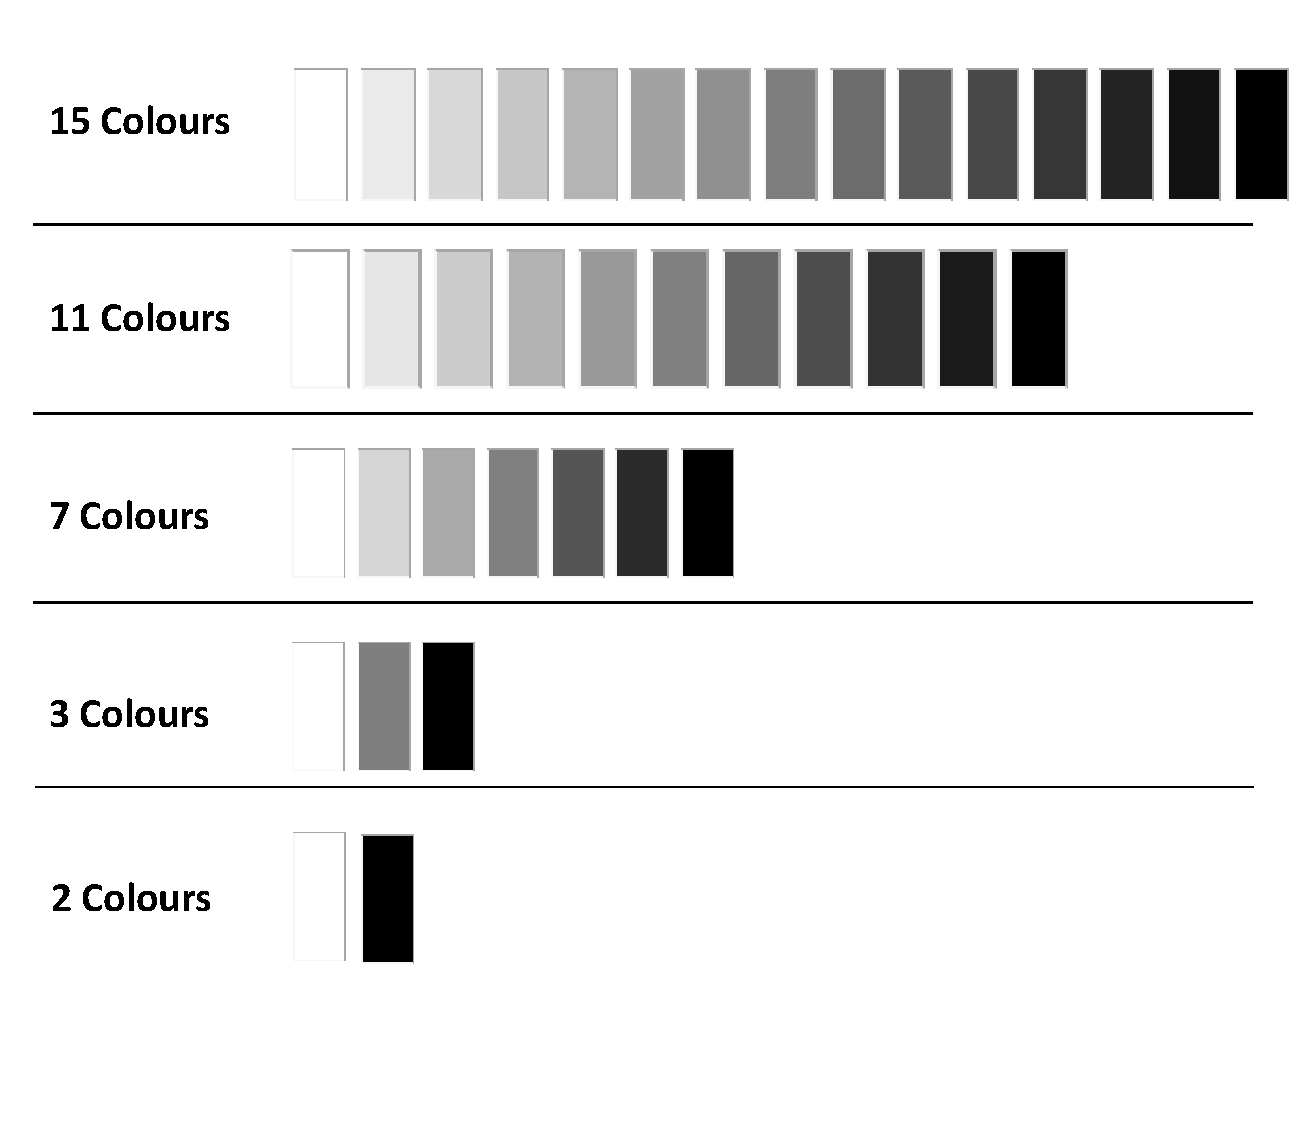
\includegraphics[width = 0.5\textwidth]{colourScheme.pdf}
\caption{Grey scale per number of colours}
\label{fig:colourScheme}
\end{center}
\end{figure} 

The colour scale is presented individually per treatment to the participant on the left of the interface (Figure \ref{fig:Interface}).
Participants can choose from 100 boxes for each round they play. The large number of boxes ensures an information overload, but still enables participants to achieve a satisfying result.
The knapsack is illustrated as a wide rectangle and is limited by its width. Boxes can be added to and removed from the knapsack by clicking on them. In the cases that a selected box doesn't fit into the knapsack because it exceeds its capacity, the knapsack will shake and appear in red, not allowing the selected box to enter the knapsack. 
 \begin{figure}[htp] % Interface
\begin{center} %Exemplary interface
  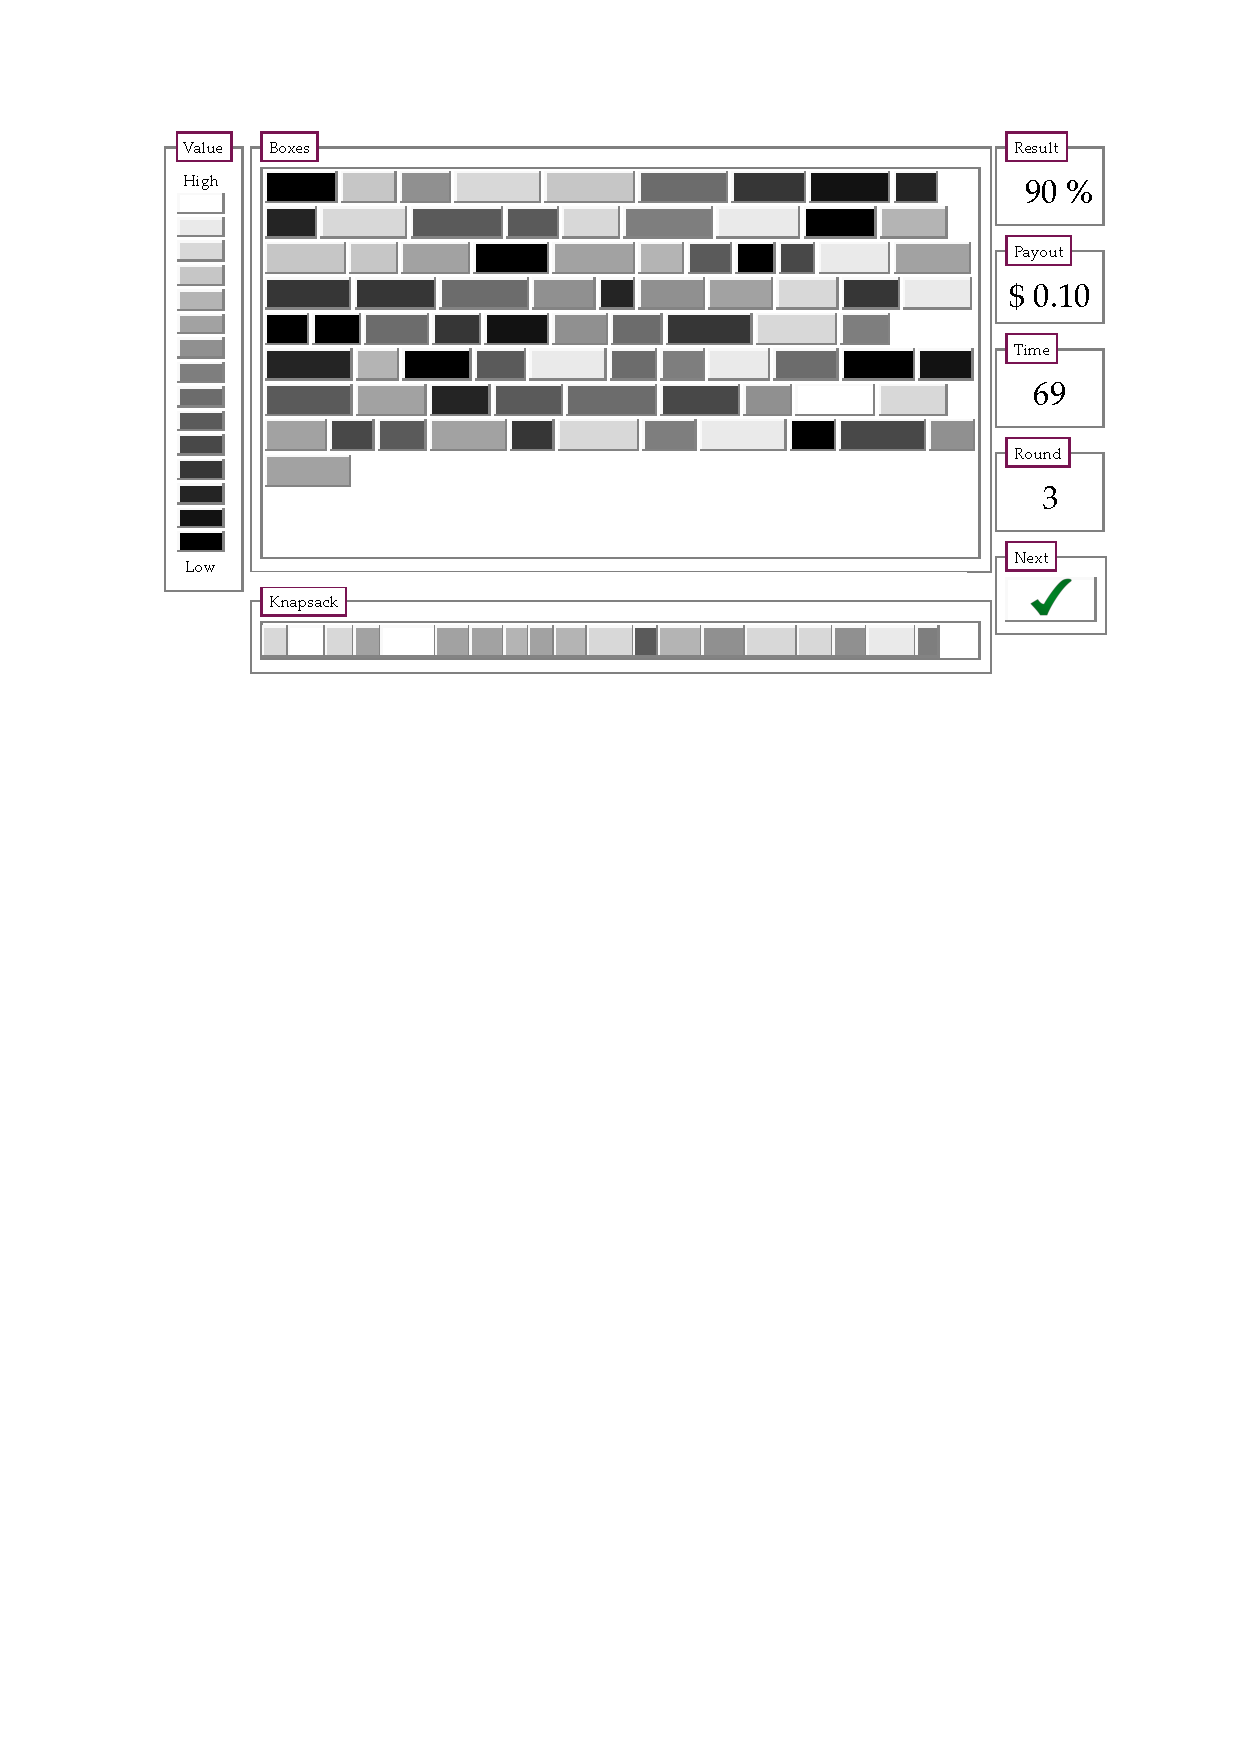
\includegraphics[height = 0.5\textwidth]{Interface4.pdf}
\caption{Exemplary interface (treatment 5, Trial 1 )}
\end{center}
\label{fig:Interface}
\end{figure} 
\subsection{Description of the toolboxes}

\paragraph{Result}

The performance of the participants is measured by comparing the current value of the knapsack to the optimal solution calculated by the \ac{DPA} introduced in Section \ref{ch:Experiment:sec:Knapsack}.
  
\begin{equation}
x = \dfrac{\text{Current value of all boxes in knapsack}}{\text{\ac{DPA} solution }}
\label{eq:x}
\end{equation}

\paragraph{Payout}

In correspondence to the result, participants receive monetary compensation for playing the current round. Every time the bonus bar \footnote{Refer to Subsection \ref{ch:Experiment:sec:Interface:subsec:Payout scheme}.} is reached, the toolbox turns green to get the participant's attention to further work on improving the result.

\paragraph{Time}
The time restriction is set to 100 seconds per round. This rather long duration is chosen because participants should not experience a significant time pressure. The main goal is to isolate the colour effect; a potential time pressure effect is not the focus of the research since time routinely has an impact on the decision quality \citep{Hahn2006}. A time limitation, however, must be implemented to ensure that it is necessary to play the round in one sitting (refer to subsection  \ref{ch:Experiment:sec:OnlineImplementation:subsec:AMT}).
The \textit{Next} button is available to give participants the opportunity to skip the current round when they have already reached a personally satisfying result and do not want to wait for the round to be finished.
\paragraph{Round}
Participants must complete three rounds. Multiple rounds are chosen to identify a potential learning effect; the limitation to three rounds keeps the total time for the experiment to a level that is attractive for an \ac{AMT} experiment. 


\subsection{Payout scheme}
\label{ch:Experiment:sec:Interface:subsec:Payout scheme}
The implemented payout scheme has two components – a guaranteed payout for each completed round and a payout dependent on the participant’s performance. A guaranteed payout is necessary to advertise the experiment on \ac{AMT} and an attractive offer draws a larger participant pool. The bonus leverage is increased in Trial 2 so the differences in the payout schemes must be taken into account in the analysis.\\
To ensure that participants would not only hit the \textit{Next}-button in each round and still get the minimum payout, a restriction is designed to only pay out participants who clicked at least one box per round.
 \begin{figure}[htp] % PayoutScheme
\begin{center}
\begin{subfigure} 
\centering
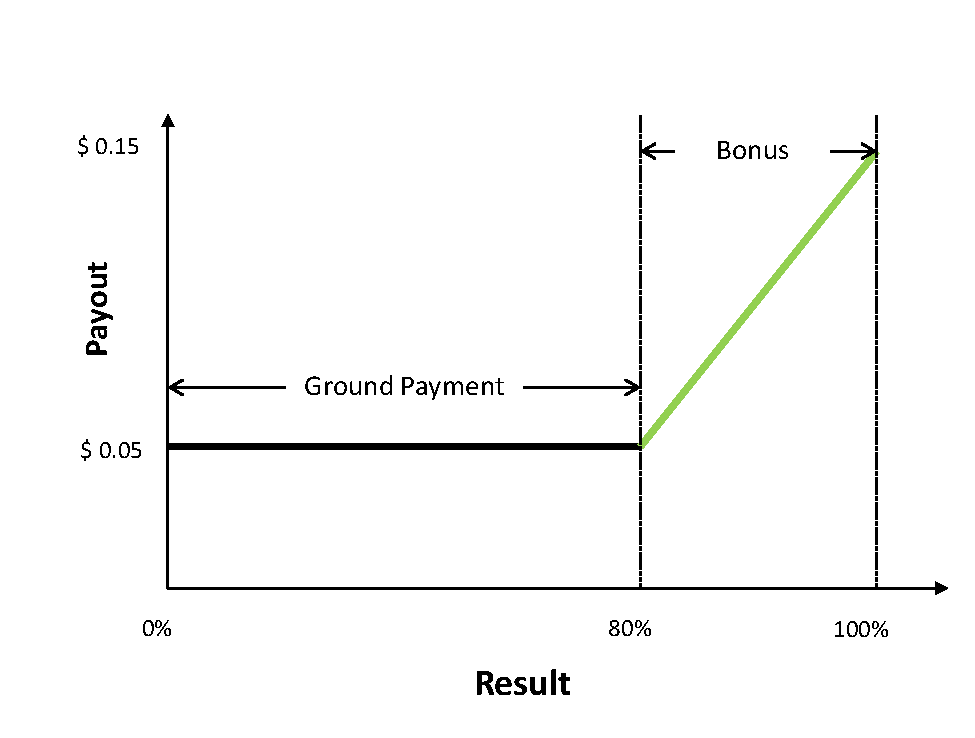
\includegraphics[height = 0.30\textwidth]{PayoutScheme.pdf}
\end{subfigure}
\begin{subfigure} 
\centering
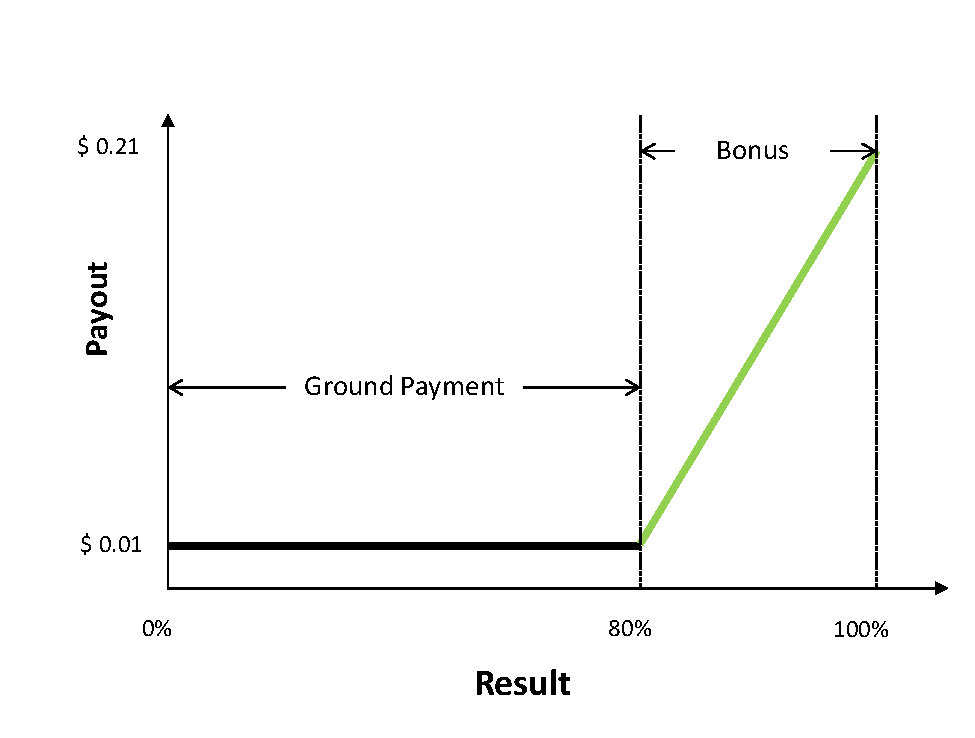
\includegraphics[height = 0.30\textwidth]{PayoutScheme2.pdf}
\end{subfigure}
\caption{Payout scheme for Trial 1 and 2}
\label{fig:PayoutScheme}
\end{center}
\end{figure} 

The reason for choosing a bonus system is caused by one goal of the experiment: get participants to compare boxes of different weights and benefits and make them try different combinations for the knapsack.
In order to incentivize such behaviour, a bonus system can help. Trial rounds show that getting up to 80\% is possible when participants make an effort and try out different solutions. Hence, the performance incentive starts at 80\% and offers the participants in the first Trial an additional bonus up to \$0.10 when reaching 100\%, resulting in a potential total payout of \$0.15 per round. Nevertheless, the experience of the first Trial shows a large number of participants who did not reach the bonus bar. Therefore, we increased the leverage of the bonus system, from a ground payment of \$0.01 to a possible total payout of \$0.21 when reaching 100\%.

%% ===========================
\section{Online Implementation}
\label{ch:Experiment:sec:OnlineImplementation}
%% ===========================

For the setup of an online environment, the Python web framework Django 1.4.3 is used to implement the communication between \ac{GUI} and the server.
The experiment is advertised on \acf{AMT} as a \ac{HIT}.

\subsection{\acl{AMT}}
\label{ch:Experiment:sec:OnlineImplementation:subsec:AMT}
A previous research study\citep{Schmidt2012} using a similar interface and setup, reached 28 participants. While the results helped to implicate that more colours to choose from does not increase the average payout, it lacked a wider statistical foundation.
Consequently, we try to increase the statistical foundation by using the online labour market \acf{AMT}.

The \ac{AMT} platform is the most active online labour market for conducting behavioural experiments. It enables researchers to conduct experiments very quickly, cheaply \citep{Rand2012}, and in good quality \citep{Gardner2012}. Moreover, the data gained is at least as reliable as the data obtained via traditional methods \citep{Buhrmester2011}. \ac{AMT} connects employers with potential workers who are paid according to the satisfactory completion of the assigned task. Furthermore, workers can be motivated to perform well by a bonus structure. Since individuals can participate entirely over the computer, the experience is quite similar to participating in computer simulations.

Researchers can act as employers on the \ac{AMT} website and offer experiments as tasks named a \acf{HIT}. Completing an \ac{HIT} usually results in a payment of less than \$1 for less than 5 minutes of work. Users are from around the world, but mainly concentrated in the United States and India \citep{Rand2012}. These findings are supported by our experiences.

\paragraph{Limitations of \acl{AMT}}
Although the \ac{AMT} offers an enormous potential for the purposes of our study, there are several limitations to keep in mind.

First, in contrast to experiments conducted in a lab environment, \ac{AMT} experiments have limited control over what kind of individuals take part in the experiment. In particular, the lack of control over \textit{non-random attrition} \citep{Rand2012} defines a limitation for our experiment in terms of the participant structure. Individuals who are overwhelmed with the complexity of the task might drop out early, do not finish the \ac{HIT} and are not included in the statistical analysis. This can have an impact on the pool of participants among different treatments and can therefore limit the ability to compare results. As a result, we have tried to make the description of the game and the game itself as simple and intuitive as possible in order to reduce the risk of early drop-outs. Trial runs previous to offering the \ac{HIT} revealed that using the Trial round helped individuals to get a better understanding of the game and the task.

Second, researchers cannot be sure as to what participants are actually doing during the experiment on the \ac{AMT} platform. This fact especially reduces the benefit to cognitive load experiments similar to our experiment since our experiment necessitates the full attention of individuals. We try to tackle this issue by setting a time restriction per round so individuals have an incentive to stay on task. Moreover, we log the time individuals spend on different parts of the experiment and evaluate the participant's actions by analysing the recorded data in order to fully understand each individual's actions. Last, we take this limitation into consideration in the choice of a statistical model.

Third, the statistical analysis is based on the assumptions that every observation is independent. In the setup of our experiment, individuals are able to conduct the experiment over and over by re-directing to the start page after finishing a session. Even though repeat responding appears to be a minor concern according to \cite{Berinsky2012}, it can still potentially dilute the observation independence and the statistical value of the learning effect. We therefore record the IP address of each user when they are directed to the welcome page in order to exclude those participants who play several games successively. However, this method does not exclude those individuals who change their IP in-between experiments.
Moreover, the \ac{AMT} platform has other disadvantages against a lab experiment in terms of user support during the experiment, and the lack of control over the English language competencies of individuals. 

After summarizing the benefits and limitations of the \ac{AMT} platform, we conclude that \ac{AMT} is feasible for our experiment when the design and evaluation of the experiment takes the limitations into consideration.

\subsection{System design}

\cite{Rand2012} indicates that in order to conduct an experiment using a game environment on \ac{AMT}, researchers must provide participants with instructions, making sure they understand the rules of the game. Next, researchers must process the data and pay the participants according to their earnings. We follow this setup for our experiment (refer to Figure \ref{fig:Enfolab}).

Once the \ac{AMT} user has decided to complete the \ac{HIT}, he or she is redirected to an external web page on which the experiment is run.
When arriving at the page, the program creates an individual user who is randomly assigned to one treatment and an individual code is generated. 
Additionally, a time stamp is saved in order to track the time a user will spend on different stages throughout the experiment.

\afterpage{
\begin{landscape}
\begin{figure}[htbp] % DistributionBestResult
\begin{center} 
\caption{Design of the online environment}
\label{fig:Enfolab} 
\begin{subfigure} 
\centering
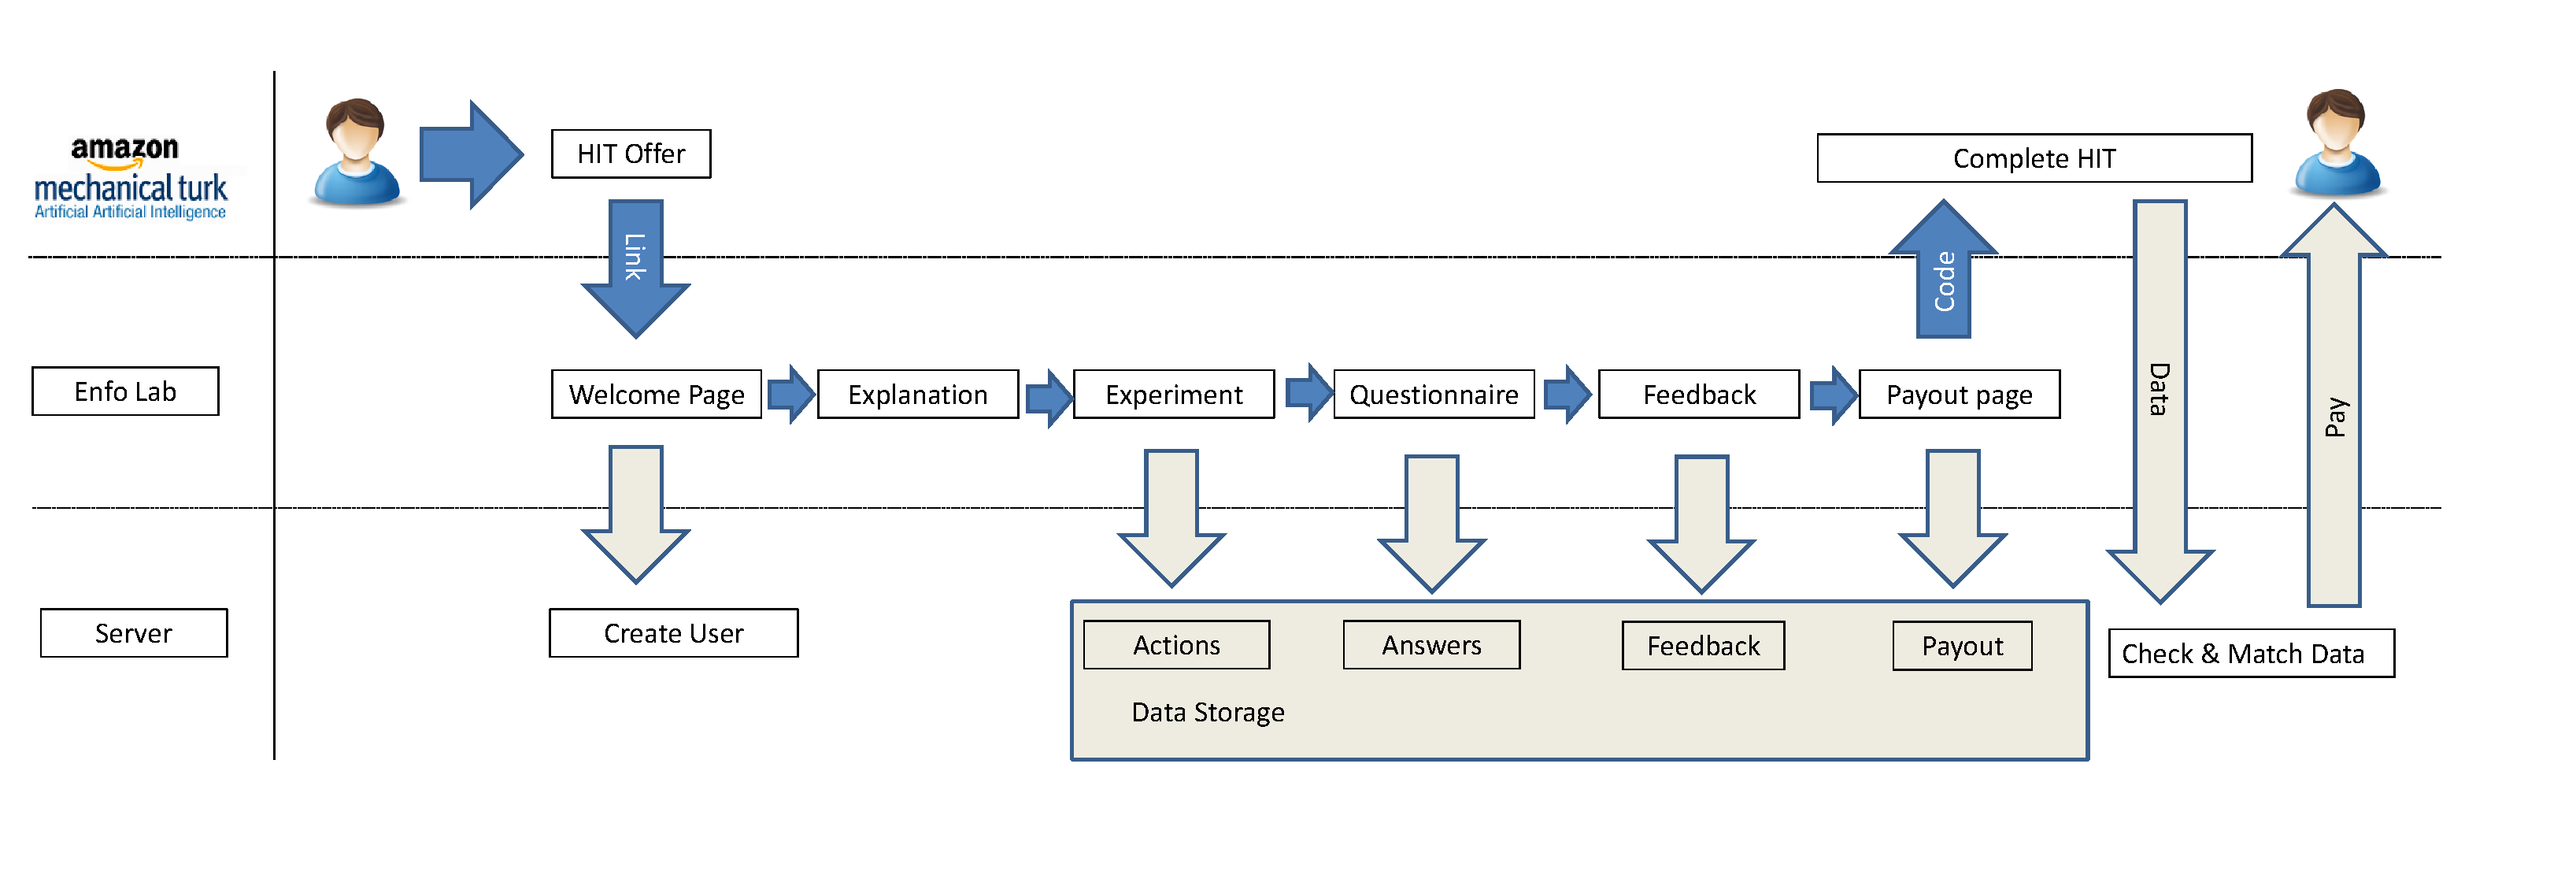
\includegraphics[width = 1.5\textwidth]{EnfoLab_Coordination.pdf}
\end{subfigure} 
\begin{subfigure} 
\centering
  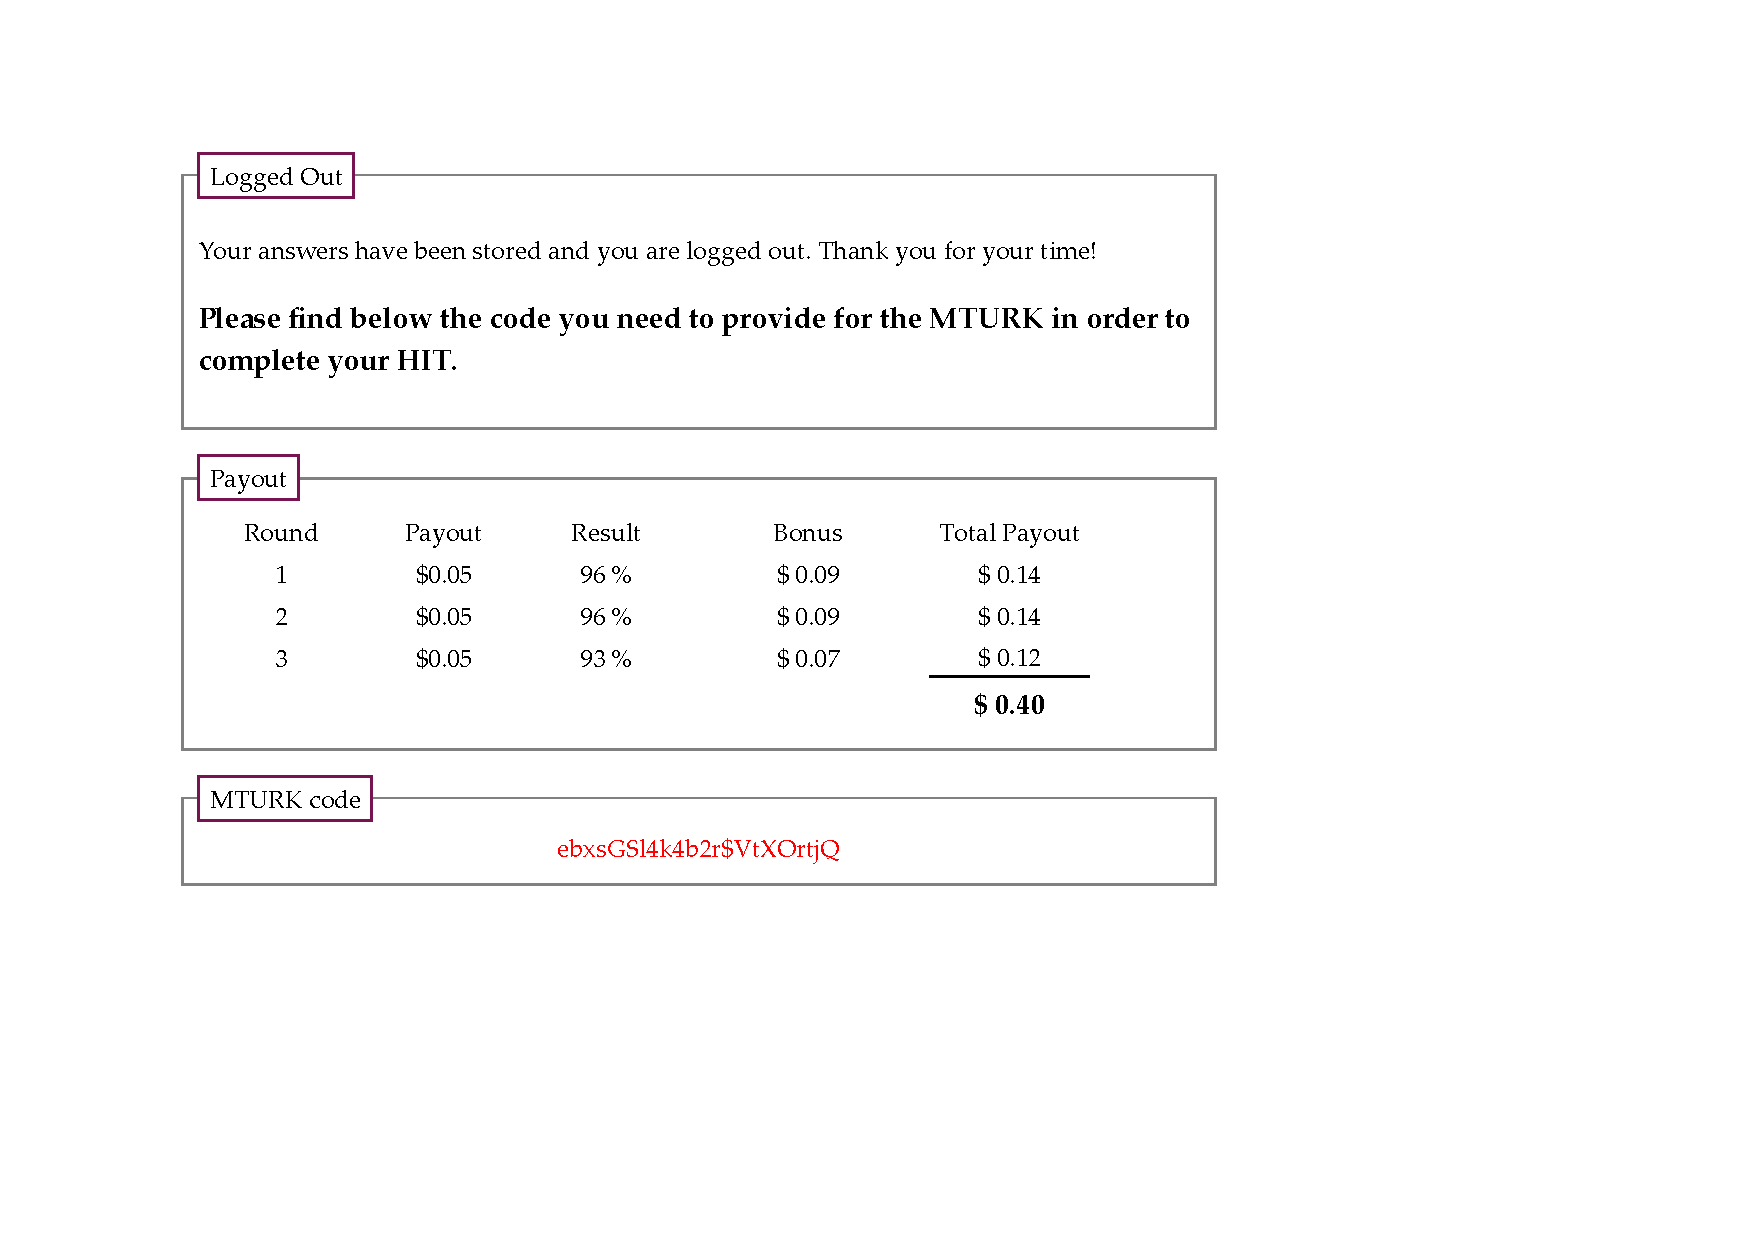
\includegraphics[height = 0.5\textwidth]{PayoutView.pdf}
\end{subfigure}
  \caption{Final page with payout}
    \label{fig:FinalPage} 
\end{center}
\end{figure}
\end{landscape}}
The participants first go through the explanation of the game where they are introduced to the concept of the knapsack problem and the implemented graphical interface. 
Before the participants begin playing their three rounds, they can get used to the interface by playing a Trial round which has no time restriction and offers information boxes to explain the different parts of the interface.\\
The participants then start the game by playing the three rounds of the experiment. Every action that includes adding or removing a box to or from the knapsack is saved on the server, including time, box ID, box benefit, box weight, current payout, the type of action (remove or add) and whether or not the knapsack is full.
The \ac{JSON} is used to transfer the determined data to the server. The collected data can be extracted from the server via a \ac{CSV} file.\\
After completing the game, participants are presented with a questionnaire where they must answer six questions about their experience playing the game and the strategy they used. To avoid participants rushing through the questionnaire, a minimum time of 15 seconds is introduced. If participants spend less time on the questionnaire, they are redirected to the beginning of the questionnaire. In addition, we include an additional question in Trial 2 that is directed to evaluate the participant's attention, by asking them to give a specific answer to the question.\\
Subsequent to the questionnaire, participants have the opportunity to give feedback by filling in a text box. This feedback is used to have an additional feedback channel to identify problems in any aspect of the interface.

The final payout for the experiment (Figure \ref{fig:FinalPage}) is shown to the participants after they have completed their three rounds and the questionnaire. 

When the minimum requirement of clicking at least one box per round is fulfilled, participants are presented the payout for each round and the total payout. Furthermore, the \ac{AMT} code is provided.
The user then goes back onto the \ac{AMT} system, enters the \ac{AMT} code and completes his or her \ac{HIT}.

At the end, the data on the server is compared to the \ac{HIT}s completed, and the payout is made via the \ac{AMT} system.

%% ===========================
\section{Data acquisition and Descriptives}
\label{ch:Experiment:sec:DataacquisitionDescriptives}
%% ===========================
The 1\textsuperscript{st} Trial was offered on \ac{AMT} between the 20\textsuperscript{th} and the 21\textsuperscript{th} of February 2013 and reached 200 participants, the 2\textsuperscript{nd} Trial with the same amount of participants ran between the 5\textsuperscript{th} and the 8\textsuperscript{th} of March 2013. A total of 31.291 actions were recorded on the server.\\
Before the data is statistically analysed using IBM's \textbf{SPSS} and \textbf{R}, the recorded data is cumulated on a per round basis for the purposes of this study. For each round per user, a data point is created that includes information on the user, treatment and corresponding number of colours, round, first result, best result, \textit{FinalResult} and finally the time for each result.
 \begin{figure}[htp] % Interface 1
\begin{center} %Exemplary interface
  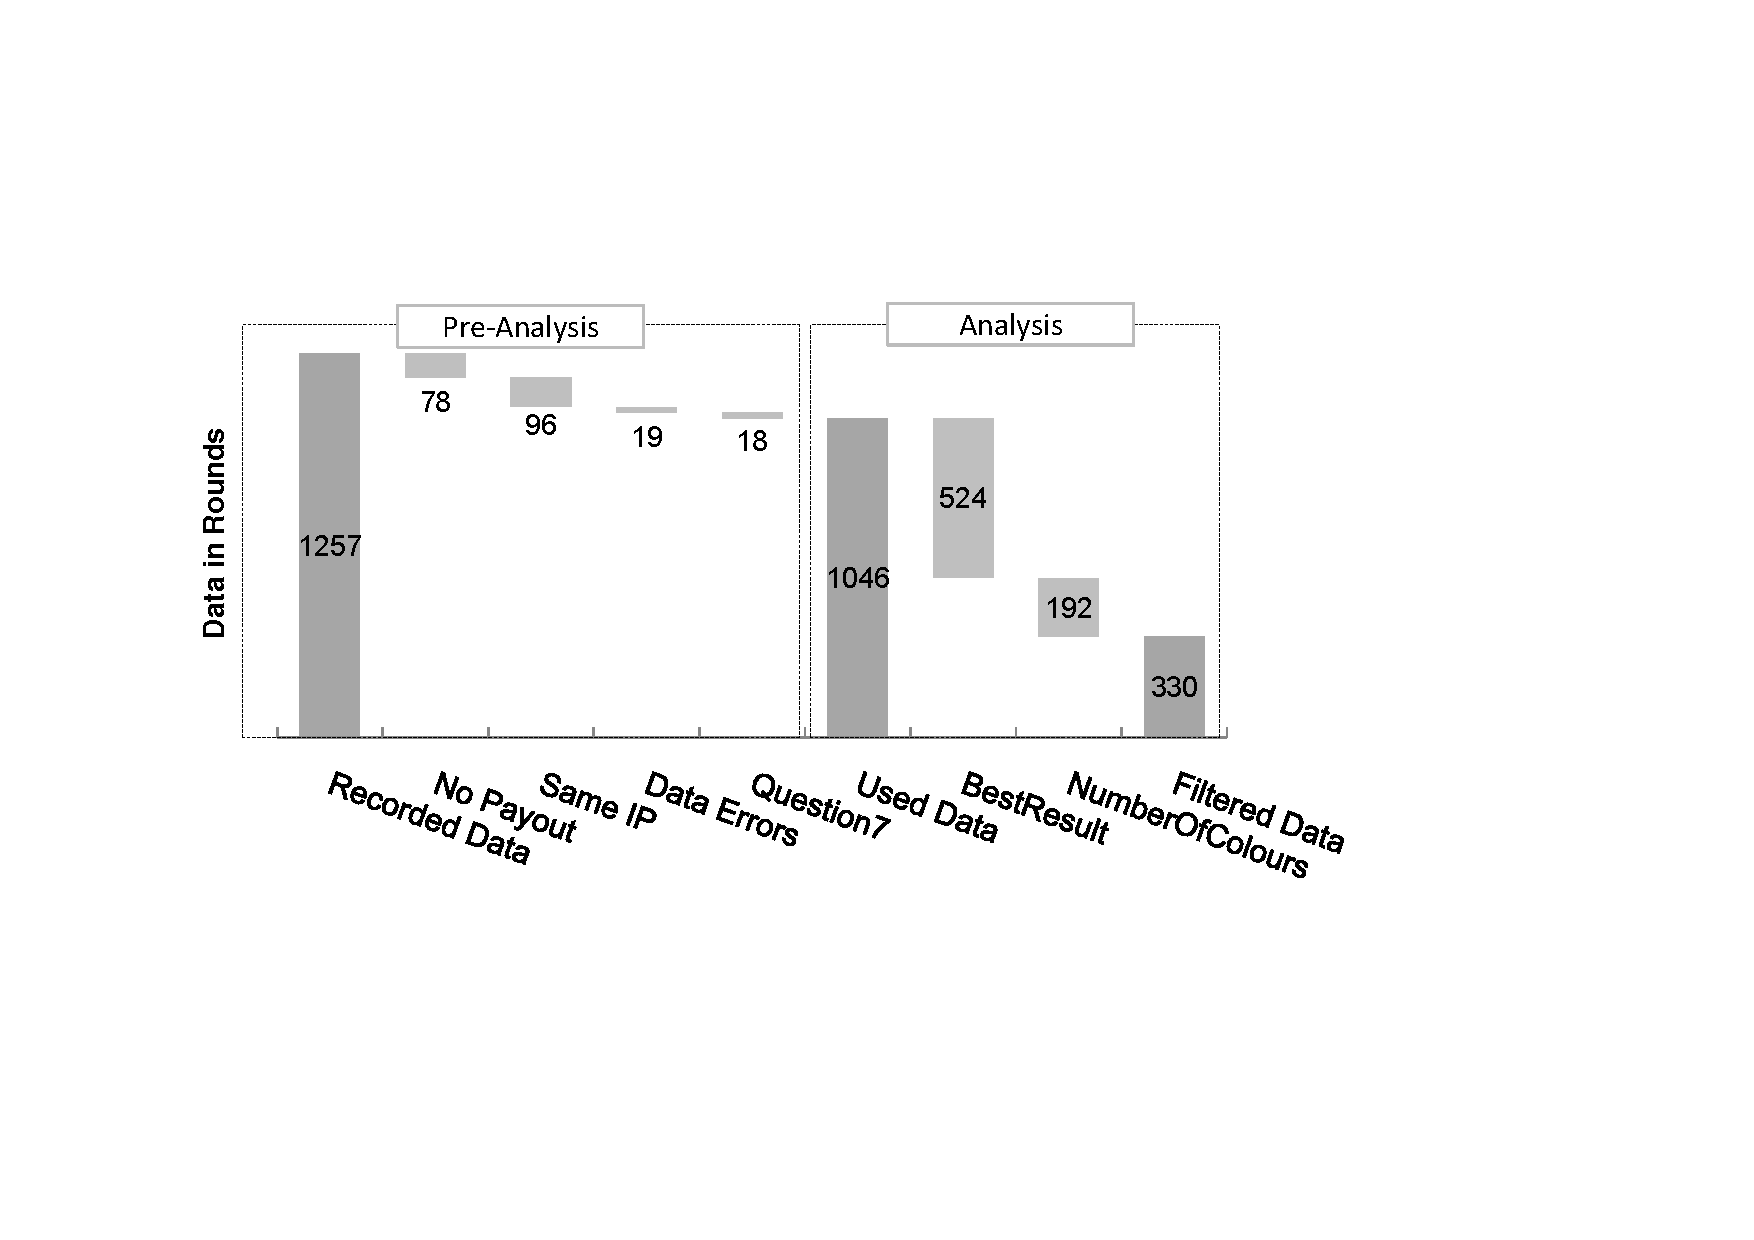
\includegraphics[height = 0.5\textwidth]{User_Waterfall.pdf}
  \caption{Generated Data in Rounds}
  \label{Data}
\end{center}
\end{figure}
Out of the 400 participants there are 1.257 played rounds recorded (refer to Figure \ref{Data}). The fact that the recorded number of rounds outnumbers the potential 1.200 rounds from 400 participants, can be explained explained using two cases. First the functionality test rounds conducted by the research team while the game was running and second by participants playing one or two rounds, then dropping out of the experiment. These cases can be identified by looking at the payout of the user, since there was no payout made to users who did not complete all rounds. Consequently, we will exclude the rounds of those users who did not achieve a payout greater than 0.\\
The next step is to identify the users who played the game again and again, and have skewed the observation independence as described in Section \ref{ch:Experiment:sec:OnlineImplementation:subsec:AMT}. 32 users are found who share both their IP with at least one other user and who achieved a payout greater than 0. The payout filter does not exclude those users who committed only once to the experiment and therefore only reached a payout greater than 0 once. \\
The data of 6 participants showed errors, e.g. a total game time per round greater than 100s or a result greater than 100\%. Since we were not able to trace the origin of these errors, we will exclude these users from the data set.
As a result, 349 users with a total of 1046 rounds build the data for the statistical analysis.\\
Within the data used for the analysis, there are two further filters applied.
These filters are used to focus on the participants who made an effort to succeed in the game. As stated in Section \ref{ch:Experiment:sec:DataacquisitionDescriptives:subsec:DescriptiveStatistics}, a performance lower than 80\% per round can be explained by a lack of effort or understanding on the participant's side. By including the whole range of performances in the parameter estimation, the statistical noise might dilute the inductive value of the study. Consequently, we only concentrate on participants who were able to achieve a result greater or equal to 80\% for each round. This filter leaves a data set is consisting of 174 users with a total of 522 rounds recorded. We will refer to this filter as \textbf{Filter 1}.\\
In a second step, users who are assigned to a treatment group with less than 7 colours are excluded. This is due to statistical implications of the data since significant results can be seen for the three remaining treatments. After applying both filters, the data sets is made up by 110 users with 330 rounds recorded. We will refer to this data set as \textbf{Filter 2}.
%
%
%Before starting the analysis, an additional implication of \acf{AMT} is taken into consideration. Cognitive load experiments conducted to the \acf{AMT} platform run the risk that users might not commit their full attention on the task (rf. to Section \ref{ch:Experiment:sec:OnlineImplementation:subsec:AMT}) and therefore may experience a different information overload than the users who give their full attention to the task. We try to determine these users by looking at the time it takes them to fill up the knapsack for the first time. Users who just randomly select boxes and quickly fill up the knapsack have a very low time until they first reach a full knapsack. A time border of 5 seconds is chosen to separate these users and the filtered data is excluded from the data set.
%Our final data set includes 536 recorded rounds from 180 users, and includes 12.929 actions.
%
%
%
%

%% ===============================
\paragraph{Experiment stages}
%% ===============================
 \begin{figure}[htbp] % Timelog
\begin{center} %Timelog
  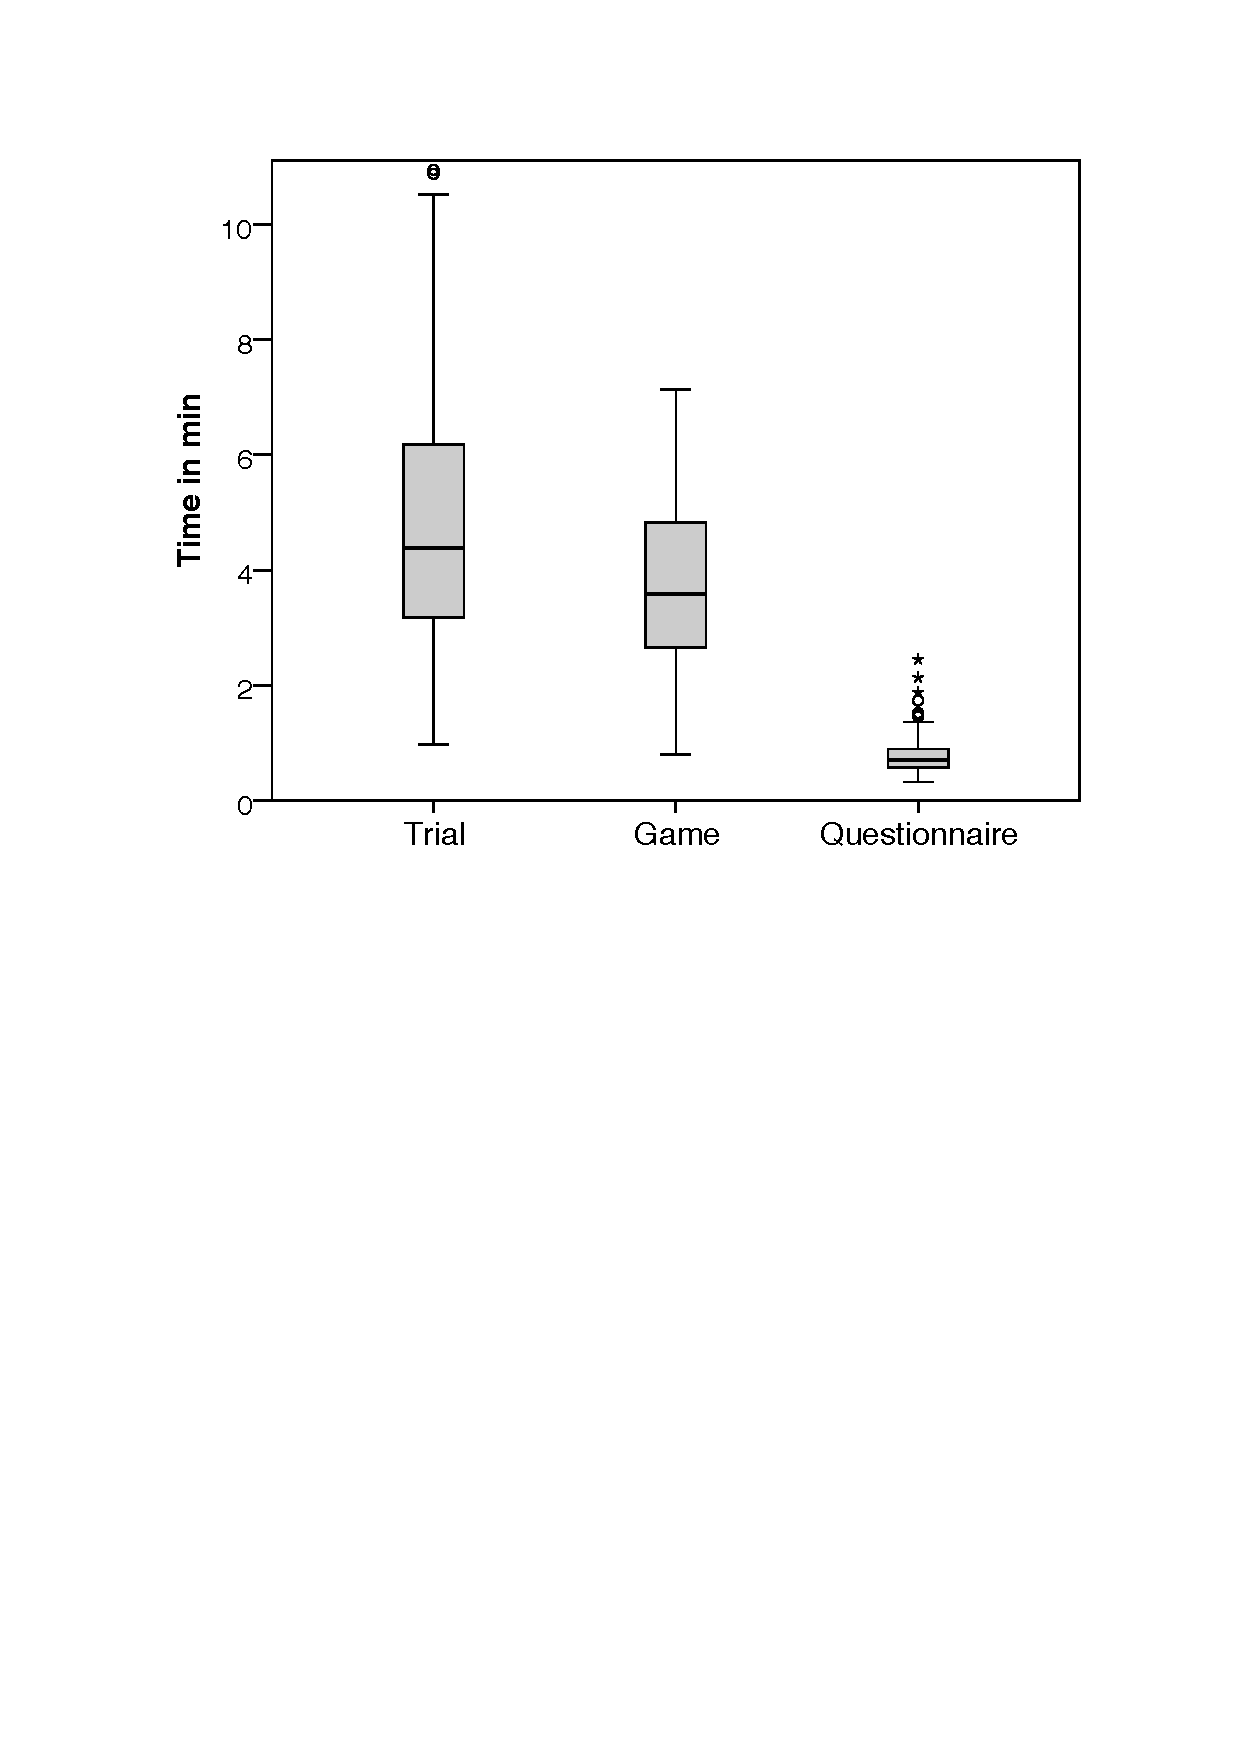
\includegraphics[height = 0.4\textwidth]{Timelog.pdf}
  \caption[Time spent on different stages of experiment]{Time spent on different stages of experiment\footnotemark}
  \label{Time spent on different stages of experiment}
\end{center}
\end{figure}
\footnotetext{Outliers with a time greater than 11 minutes on each stage are excluded for the purposes of this graph due to better readability. }

The tracked time logs for the participants  (Figure \ref{Time spent on different stages of experiment}) show that individuals spent a considerable amount of time on the explanation and the Trial round. The total game length is defined by 5 minutes, and the majority of participants complete the game in less than the maximum time. A value greater than 5 minutes can be explained by the information box that pops up before the beginning of the game. The countdown for the current round only starts after participants click on the information box to start the round, resulting in a total game duration longer than 5 minutes when participants do not click instantly on the info box.
The questionnaire is the shortest of the stages. We set a minimum time of 15 seconds, corresponding to .25 minutes, to fill out the questionnaire - the majority of individuals spent between 30 to 60 seconds on the questionnaire section.

%% ===============================
\paragraph{Feedback from participants}
53\% of all users used the opportunity to give feedback via text. The majority gave positive feedback on the technical functionality of the game. These results might, however, be skewed since the feedback page is only reached by participants who did not have any major technical problems while going through the experiment. \\
Only a small number of participants gave feedback on areas of improvement, including the suggestion to offer a better and earlier visual notification when the time is running out. One participant suggested to introduce a more colourful colour scale or background music.


%% ===============================
\section{Data Descriptives}
\label{ch:Experiment:sec:DataacquisitionDescriptives:subsec:DescriptiveStatistics}
%% ===============================

This section aims to provide a descriptive overview of the unfiltered data. First, the treatment statistics are introduced, second the descriptive results from the game are analysed and third the answers from the participants are examined.
%% ===============================
\paragraph{Treatments and payout}
\label{ch:Evaluation:sec:DescriptiveStatistics:subsec:Distributionoftreatments}

The participants were randomly and uniformly assigned to one treatment once they directed to the welcome page. The low share of treatment 1 is related to the fact that the treatment was added in Trial 2 (Table \ref{Distributionoftreatments}).\\ 
\begin{table}[htbp] % Distribution of treatments
  \centering
  \caption{Distribution of Treatments}
    \label{Distributionoftreatments}
    \begin{tabular}{ccccc}
    \toprule
    \multirow{2}[1]{*}{Treatment} & \multirow{2}[1]{*}{Users} & \multirow{2}[1]{*}{Share} & Share of  & Share\\
    						   &						&  						 &	Dropouts\footnotemark & Minimum Payout\\
    \midrule
    1     & 33    & 10\%  & 37\% & 31\%\\
    2     & 88    & 25\%  & 40\% & 25\%\\
    3     & 78    & 22\%  & 40\% & 31\%\\
    4     & 72    & 21\%  & 39\% & 28\%\\
    5     & 77    & 22\%  & 46\% & 27\%\\
    
    \bottomrule
    Total & 348   & 100\% & 40\% & 28\%\\
    \end{tabular}%
\end{table}%
\footnotetext{See Appendix \ref{Appendix-Formulas} for the formulas.}

The distribution of payout presented in Figure \ref{Distributionofpayout} shows that the medians of the payout per treatment is decreasing with the \textit{NumberOfColours} in Trial 1, whereas an inverted U-Shape can be detected for the medians in Trial 2, with a peak at the medium 7-colours level.\\
28\% of all users achieved the minimum payout of each Trial, and 72\% reached the bonus bar. The highest payout is \$0.44 accomplished in Trial 1, and \$0.55 in Trial 2. 

 \begin{figure}[htbp] % Distributionofpayout
\begin{center} 
  \caption{Distribution of payout among treatments for each Trial}
    \label{Distributionofpayout}
  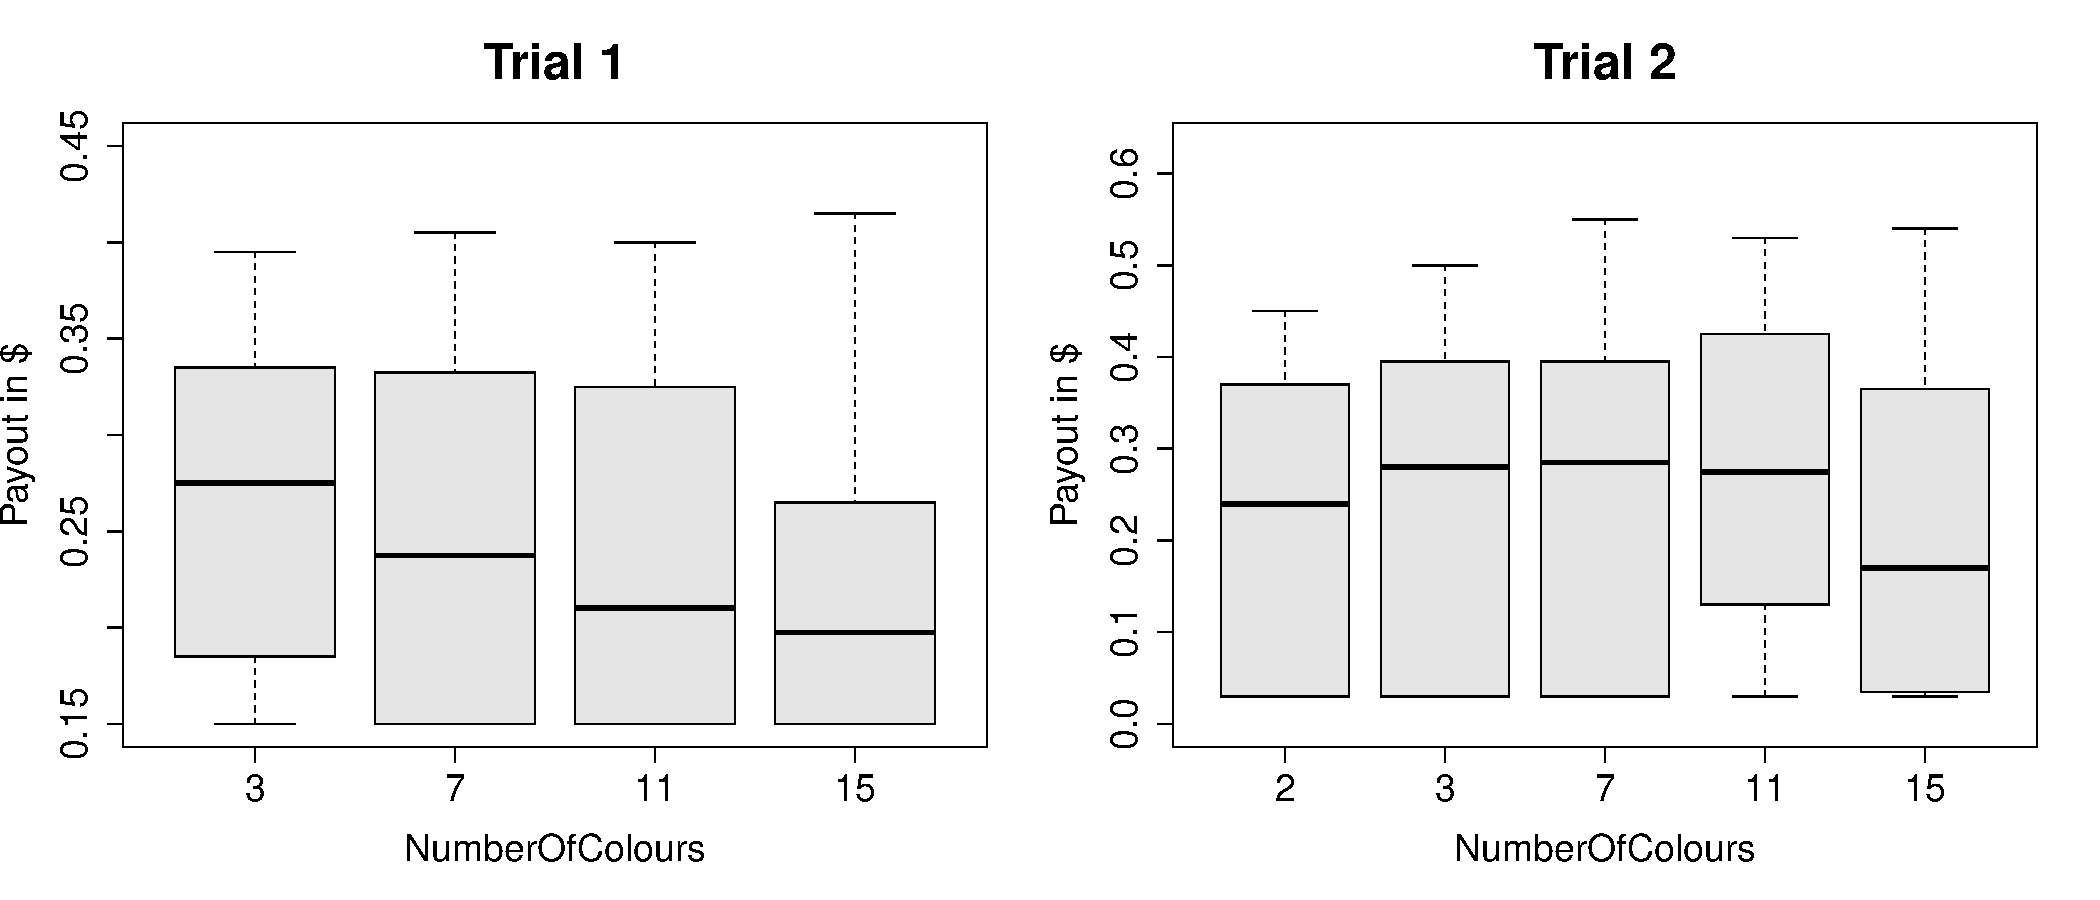
\includegraphics[width = 1\textwidth]{DescriptivesPayout.pdf}
\end{center}
\end{figure}
%% ===============================
\paragraph{Performance}
\label{ch:Evaluation:sec:DescriptiveStatistics:subsec:Performance}
The characteristics of the histograms for all result types show a similar shape\footnote{Figure \ref{DistributionFinalResult} (left) shows the histogram for the \textit{FinalResult}, see Appendix \ref{Appendix-Descriptive} for Histograms and Boxplots for \textit{FirstResult} and \textit{BestResult}.}. The average result lies between 75\% for the \textit{FirstResult} and 79\% for the \textit{BestResult}. The relative standard deviation is high with values greater than 23\%, and the standard deviation is just below 20. 
The population for all result types are negatively skewed with a value between --1.29 and --1.58, and the kurtosis is positive in the range of 1.4 and 2.4. The modal group can be found between 85\% and 95\%.\\
As indicated by the histograms, there is a lot of noise in the data, where values below 80\% are likely to be related to a minimum effort. Therefore, the statistical potential by excluding the low performers is emphasized.
The distribution of the different result types among different treatments is exemplary, as shown in Figure \ref{DistributionFinalResult} (right) for the \textit{FinalResult} and indicates a decreasing interquartile range with an increasing number of colours. The medians for all treatments are above the bonus bar and show a tendency to form a U-Shape with a peak at the treatment with three colours.\\
\begin{figure}[htbp] % DistributionFinalResult
\begin{center} 
  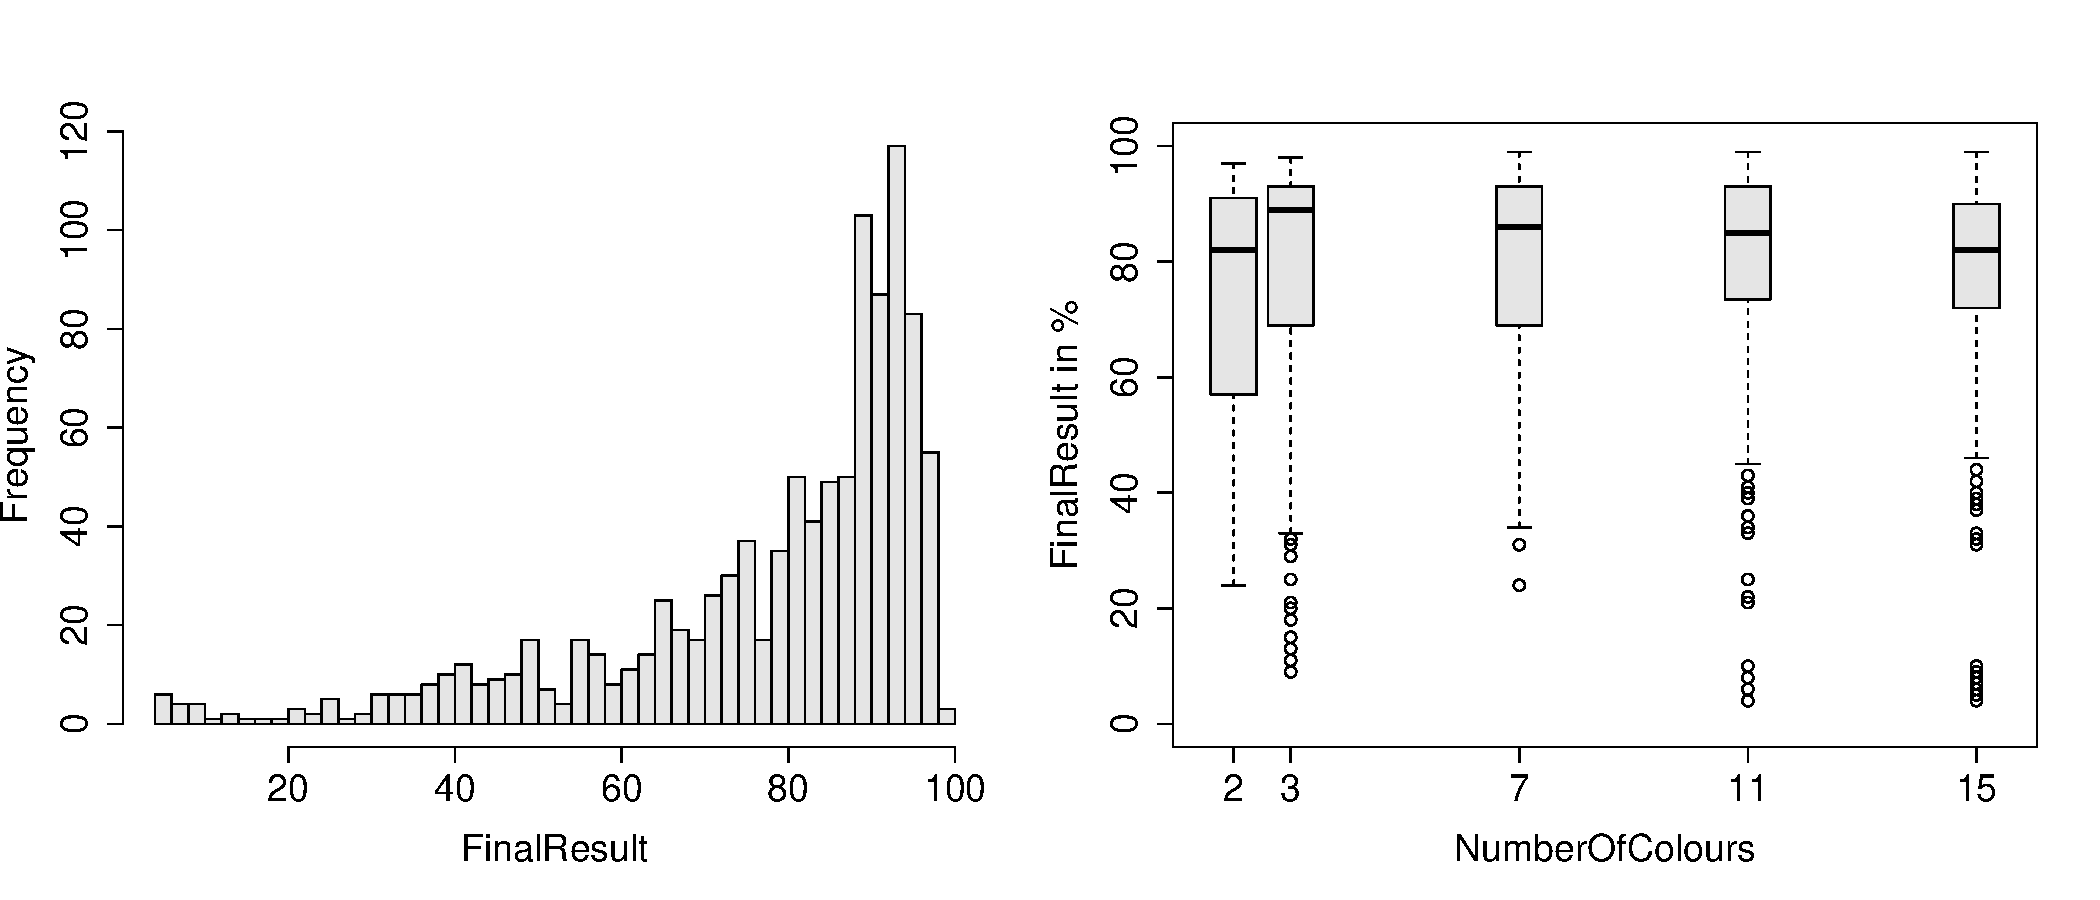
\includegraphics[width = 1\textwidth]{DescriptivesFinalResult.pdf}
  \caption{FinalResult - Histogram and Box plot}
    \label{DistributionFinalResult} 
\end{center}
\end{figure}
Significant outliers can be found in all treatments except for the treatment with two colours. Outliers with a \textit{FinalResult} lower than 20\% can be explained by a lack of effort and understanding on behalf of the participant, as opposed to an experience of information overload. A result greater than this value can namely be achieved by simply clicking on random boxes to fill up the knapsack.

\paragraph{Time}
\label{ch:Evaluation:sec:DescriptiveStatistics:subsec:Time}
The histograms of the different time types differ. Whereas \textit{FirstTime} shows a positively skewed distribution, \textit{BestTime} seems to be close to a uniform distribution. \textit{FinalTime} has a negative skewed population and \textit{DecisionTime} looks like like the results are normally distributed. The majority of participants reached the \textit{FirstResult} under 40s, and finished the round mostly in over 80s. Since only a minority played the full time, the use of the "Next"-button seemed to be popular. No specific time can be identified when participants were most likely to reach their \textit{BestResult}.\\
\begin{figure}[H] % DistributionFinalTime
\begin{center} 
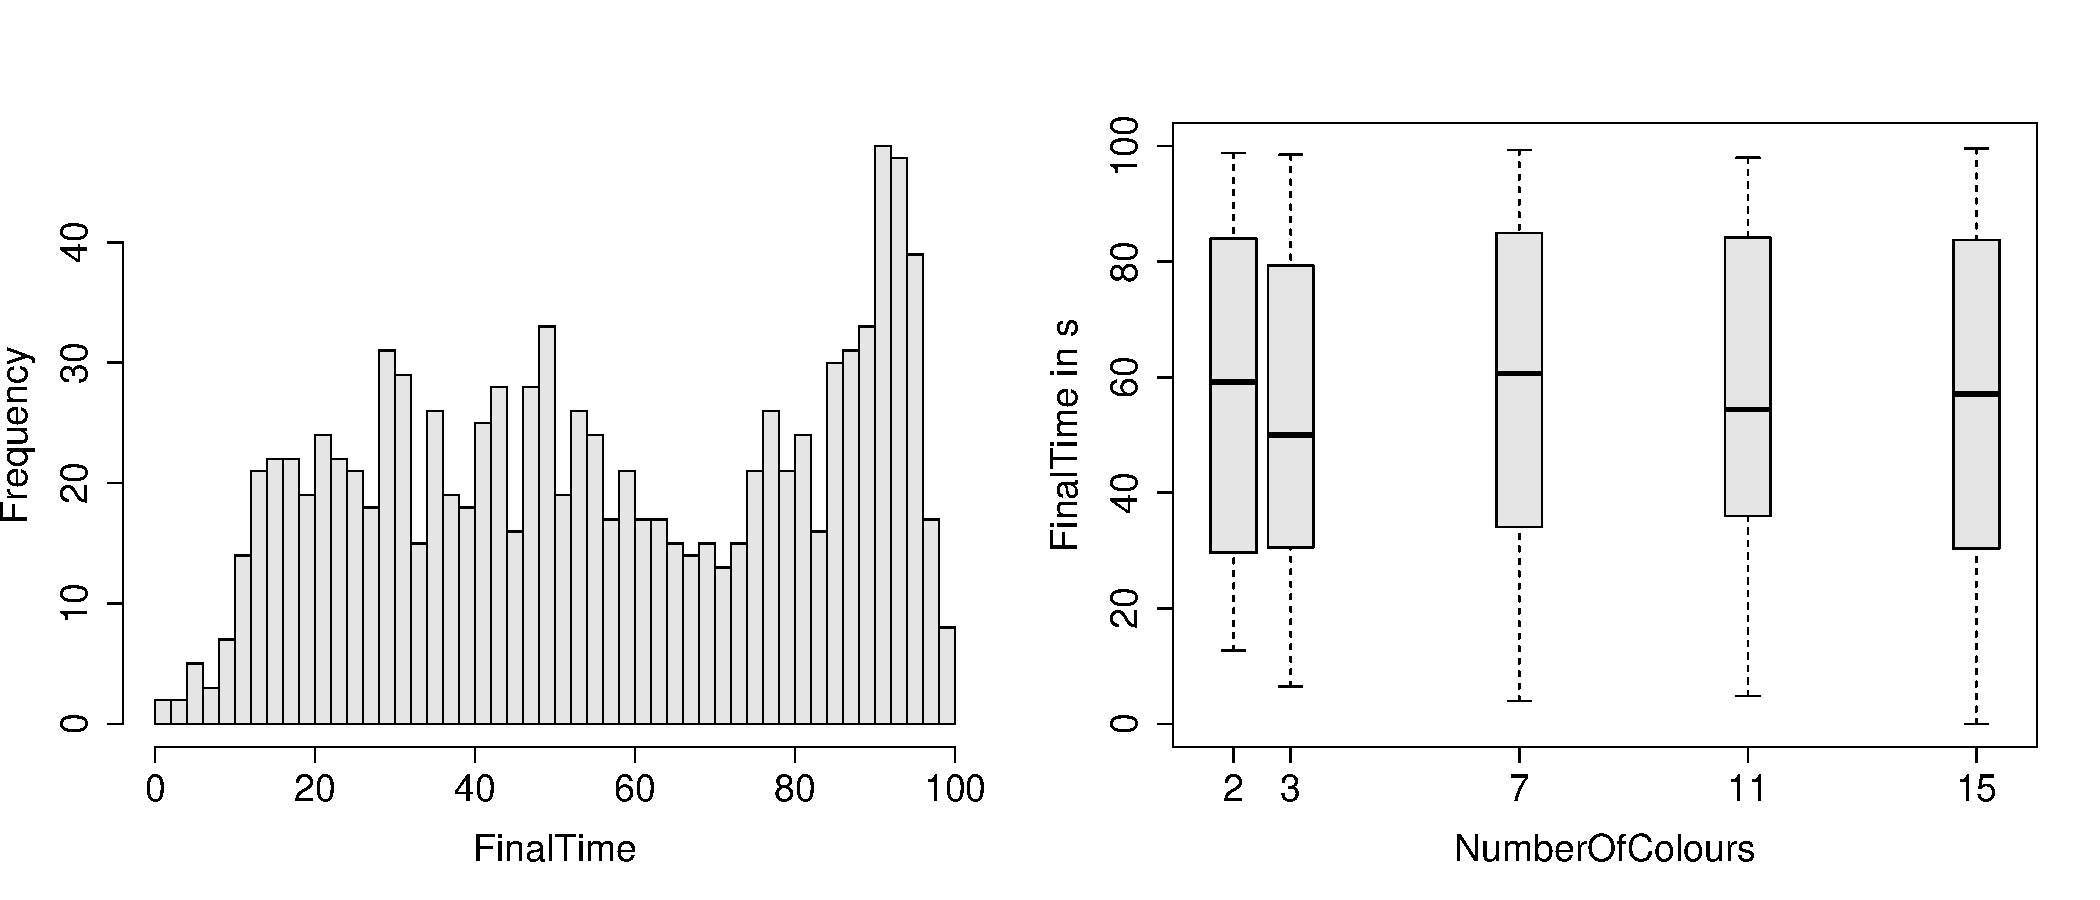
\includegraphics[width = 1\textwidth]{DescriptivesFinalTime.pdf}
  \caption{FinalTime - Histogram and Box plot}
    \label{DistributionFinalTime} 
\end{center}
\end{figure}
The box plot of \textit{FirstTime} shows similar medians across treatments. The interquartile range is smaller for treatments 2 and 4, and bigger for treatment 3. The standard deviation is the lowest for all time types.\\
The interquartile range is similar among all treatments for the \textit{BestTime}. The values for the medians define a U-shape, with treatment 2 as the apex. The medians for \textit{FinalTime} vary across treatments, yet the interquartile range does not seem to be dependent on the number of colours.\\


\paragraph{Decision time and number}
The box plots of \textit{DecisionTime} show a wide range, from below 0s to up to 6s for all treatments. The medians are similar and treatment 3 has a wider interquartile range. The majority of participants showed between 5 and 40 clicks on boxes per round. The box plot for \textit{DecisionNumber} show outliers for every treatment, resulting in a range from less than 10 until up to 90 clicks per round.

\begin{figure}[htbp] % DistributionDecisionNumber
\begin{center} 
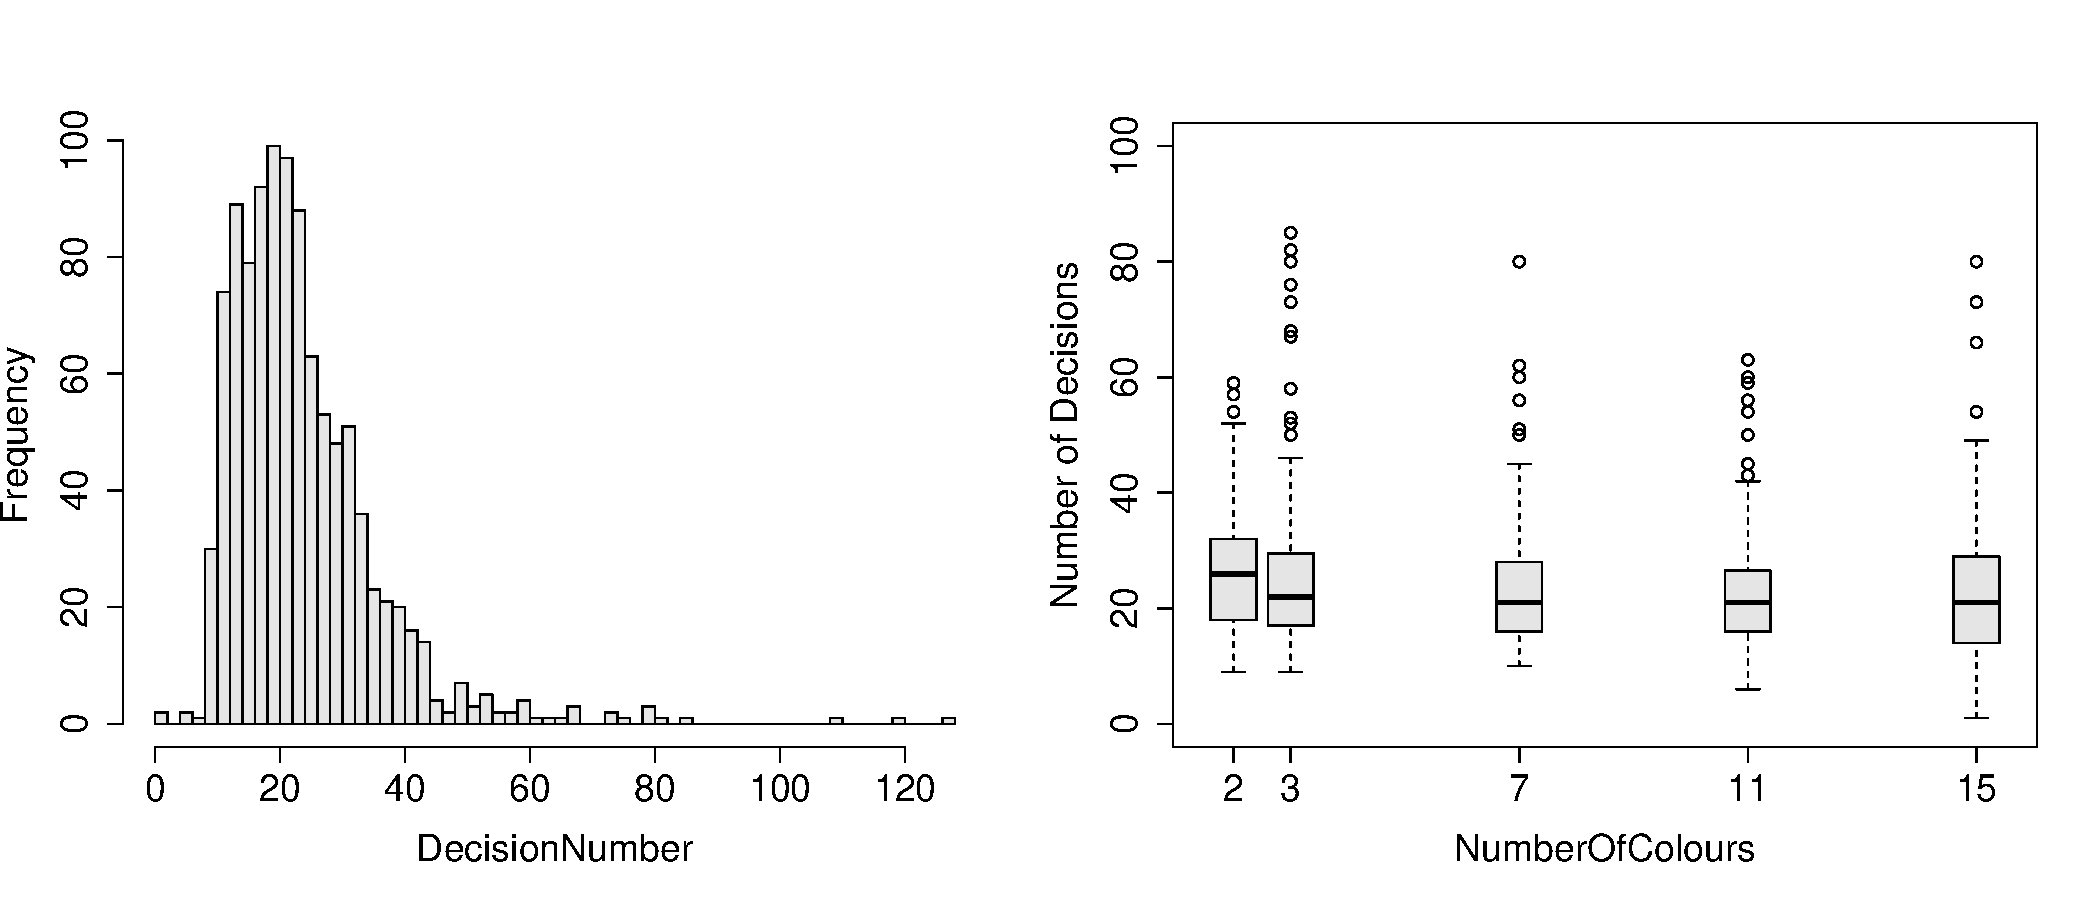
\includegraphics[width = 1\textwidth]{DescriptivesDecisionNumber.pdf}
  \caption{DecisionNumber - Histogram and Box plot}
    \label{DistributionDecisionNumber} 
\end{center}
\end{figure}

%% ===============================
\paragraph{Questionnaire}
\label{ch:Evaluation:sec:DescriptiveStatistics:subsec:Questionnaire}

Figure \ref{ProfilePlot} summarizes the medians for all the answers per treatment. In general, the medians for all treatments show similar values, so the different treatments do not seem to have an influence on the answers.\\
The mental demand for the task is described as high(5) for all \textit{NumberOfColours} and the pace of the task is defined as a medium to rather high. 
Most of the participants indicate their performance as rather successful and define their effort for accomplishing their level of performance as high.\\  
There are no significant signs for negative emotions like insecurity and irritation triggered by the experiment, since all treatments indicate a low level of negative emotions. 
Most individuals define "colour" (2) as the main box attribute they were looking at to reach their end result. A high number of individuals take into consideration a combination of the box size and box colour(3) to reach their end result.
The box size (1) is considered by only a small minority of participants, and other strategies(4) or no strategy(5) have only a minor influence on individuals. 

%\begin{landscape}
 \begin{figure}[htbp] % ProfilePlotAnswer
\begin{center} %ProfilePlotAnswer
\begin{subfigure} 
\centering
 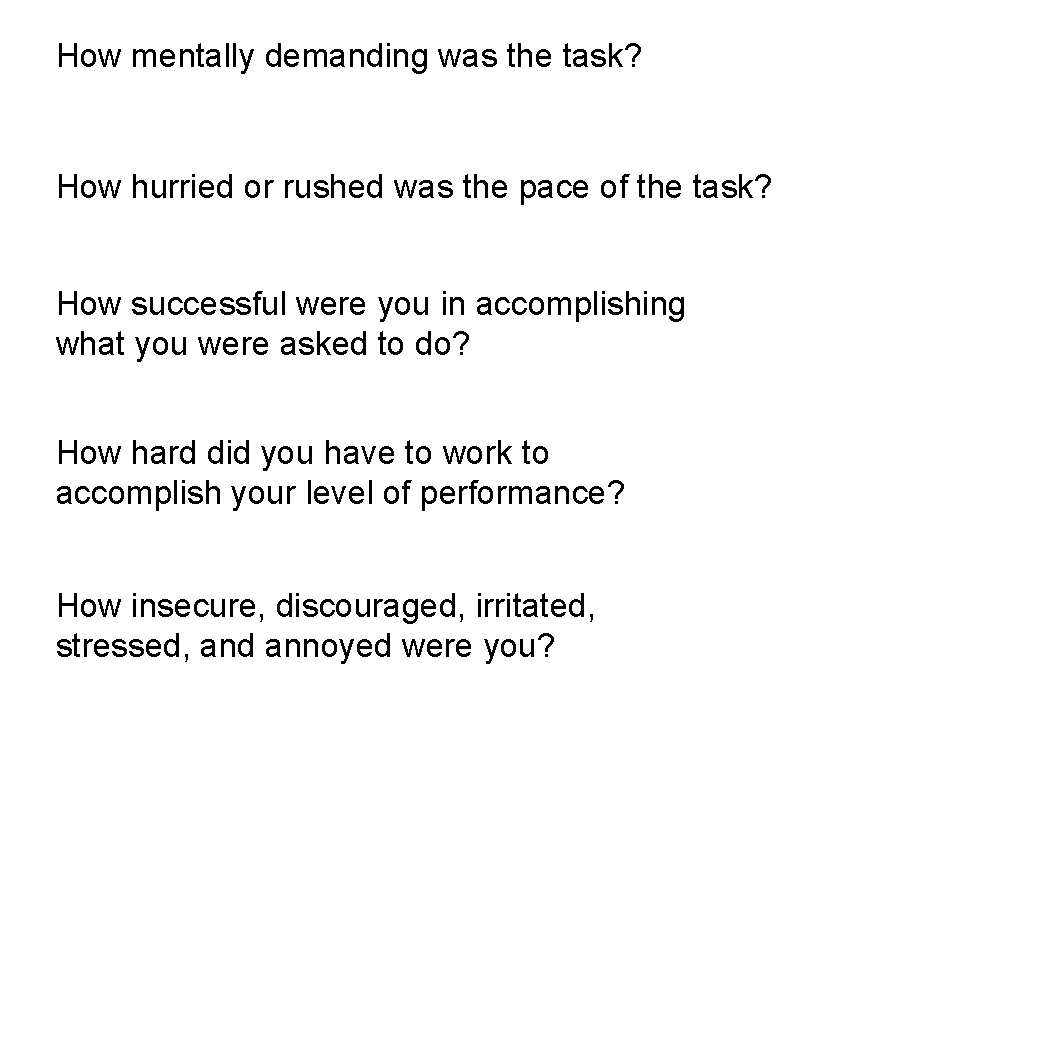
\includegraphics[height = 0.6\textwidth]{ProfilePlotLegend.pdf}
\end{subfigure} 
\begin{subfigure}
\centering
 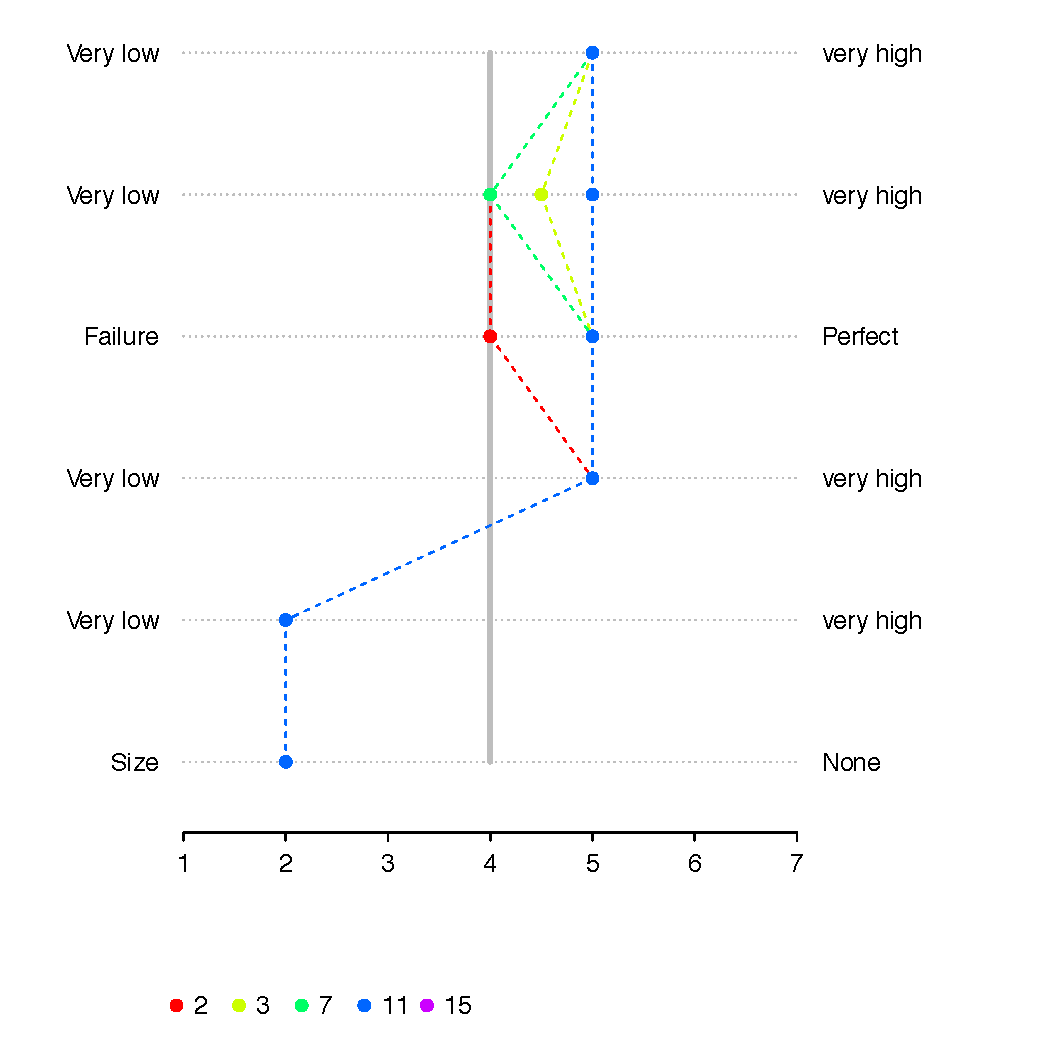
\includegraphics[height = 0.6\textwidth]{ProfilePlotAnswer.pdf}
\end{subfigure}   
  \caption{Profile Plot}
  \label{ProfilePlot}
\end{center}
\end{figure}
%\end{landscape}

% ===============================
\paragraph{Correlation of variables}
Figure \ref{Correlation} concludes the correlation between all the variables. The bigger the size of the circles, the greater the magnitude of the correlation. The green colour represents a positive correlation, the red colour represents a negative linear correlation, so big green circles refer to a high positive linear correlation.\\
The two main correlation groups which can be identified as the different result types and the different time types both show a high correlation. The correlation between these two groups is smaller, but still positive. This result indicates that the more time a participant takes for completing the round, the more successful he or she is, vice versa.\\
The linear correlation between the time and result variables, and the independent variables \textit{Round} and \textit{NumberOfColours}, is only small, yet the \textit{DecisionTime} shows a higher positive correlation for the \textit{NumberOfColours} and a negative correlation for \textit{Round}. In other words, the more colours that are added to the game, the more time it takes the participant on average to make a decision and the decision time decreases over the rounds played.\\
The \textit{DecisionNumber} is positively correlated with the result and time variables, showing the highest correlation value for \textit{FinalTime} and \textit{BestTime}.

 \begin{figure}[htbp] % 130315_CorrelationAction
\begin{center} %130315_CorrelationAction
  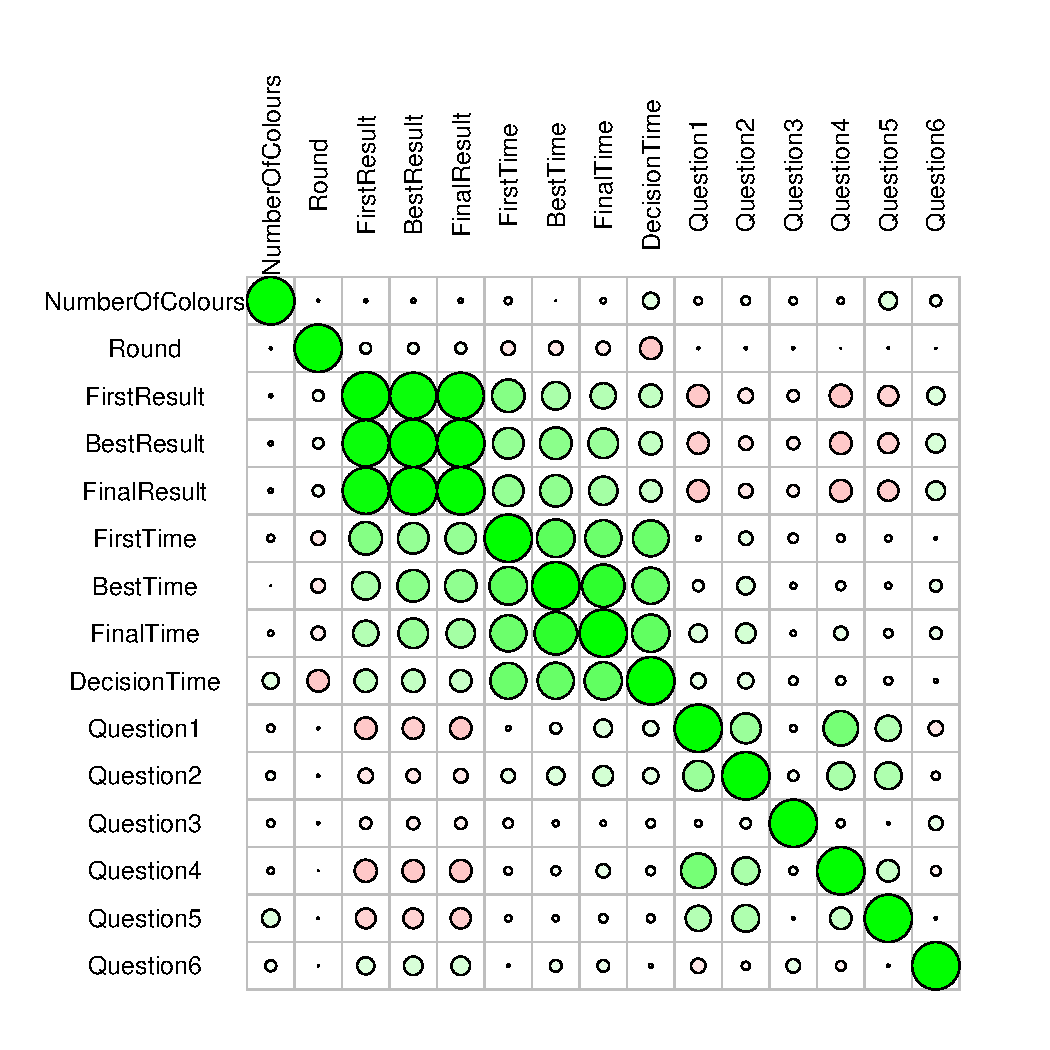
\includegraphics[height = 0.7\textwidth]{CorrelationAction.pdf}
  \caption{Correlation of variables}
  \label{Correlation}
\end{center}
\end{figure}

The correlation between the mental demand of the task (Question 1) and the level of how hard participants work to accomplish the task (Question 4) is the highest for all answers' correlations, even though it indicates only a medium correlation. Smaller but still positive correlations with the mental demand, can be identified for the pace of the task (Question 2) and the level of negative emotions (Question 5).\\
A small negative correlation is detectable for Question 1, Question 4 and Question 5, and the performance variables. Therefore, participants with a higher result indicate a lower mental demand, a lower level of effort and a lower level of negative emotions. Interestingly, the correlation matrix does not show a high correlation between how successful the participants are and how successful they feel (Question 2). 

%% evaluation.tex
%%

%% ==================
\chapter{Evaluation}
\label{ch:Evaluation}
%% ==================

The knapsack experiment which is used to test the effects of information overload on individuals is carefully evaluated in this section. In the first step we discuss the choice of statistical models, second we introduce the \acf{LMM} that is used to examine the recorded data, and in the last step we present the results for the parameter estimations. 

%% ===============================
\section{Choice of statistical model}
\label{ch:Evaluation:sec:StatisticalModel}
%% ===============================

In order to evaluate the data and extract statistical stress-able results, the appropriate choice of a statistical model is crucial. 
\cite{Siegel1957} defined three main criteria to identify the most suitable statistical model:
\begin{enumerate}
\item The statistical model of the test should fit the conditions of the research.
\item The measurement requirement of the test should be met by the measures used in the research.
\item From among those tests with appropriate statistical models and appropriate measurement requirements, that test should be chosen which has greatest power-efficiency\footnote{The power of a test is being defined as the probability that the test will reject the null hypothesis when in fact it is false and should be rejected \citep{Siegel1957}. Thus, a statistical test is considered to be good if it has small probability of rejecting $H_0$ when $H_0$ is true, but a large probability of rejecting $H_0$ when it is false.}.
\end{enumerate}

The conditions of the research are defined by a combination of two between-subjects and one within-subjects factors. \textit{Usergroup} and \textit{Trial} separate the treatments and the within-subjects factor \textit{Round} defines the number of observations recorded for each subject.
Table \ref{tab:OverviewVariables} gives an overview of the examined variables. All variables fulfil the measurement requirements since all dependent variables are numerical and on a scale, and all independent variables are numerical and ordinal. \\
% Table generated by Excel2LaTeX from sheet 'Tabelle2'
\begin{table}
  \centering
    \begin{tabular}{l|lll}
    \toprule
    \multicolumn{1}{c|}{Independent}  & \multicolumn{3}{c}{Dependent} \\
    \midrule
    \textit{NumberOfColours} & \textit{FirstResult} & \textit{FirstTime} & \textit{DecisionTime}\\
    \textit{Round} & \textit{BestResult} & \textit{BestTime} & \textit{DecisionNumber}\\
    \textit{Trial} & \textit{FinalResult} & \textit{FinalTime}\\
    \bottomrule
    \end{tabular}%
      \caption{Overview - Independent and dependent variables}
    \label{tab:OverviewVariables}%
\end{table}%

Two statistical models are chosen to examine the data.\\
The application of \acf{NP} is aimed at answering whether or not there is an influence from the independent variables \textit{NumberOfColours} and \textit{Trial} on the dependent variables. In particular, the different filters are tested to identify the data sets that show an influence on \textit{NumberOfColours} and \textit{Trial}.\\
Subsequently, a \acf{LMM} is used to give parameter estimations to the combination of those dependent and independent variables that show an influence in the \ac{NP}s.

%%% ===============================
%\section{\acf{GLM}}
%\label{ch:Evaluation:sec:GLM}
%%% ===============================

%The implemented statistical model has two components, the structural part defines the patterns of means for each usergroup. The error model describes the variability of users within usergroup around the mean. The deviations of individual measurements are assumed to be independent.

%A \acf{GLM} is first applied to examine the hypotheses. \ac{GLM}s are considered to be powerful tests since their assumptions are very strong. Moreover, they fit the conditions of our research, since they can combine two different types of factors, between-subjects and within-subjects factors.\\
%There is one between-subjects factor, \textit{Usergroup}, that separates the treatments and one within-subjects factor, \textit{Round}, that defines the number of observations recorded for each subject.


%\afterpage{
%\begin{landscape}
%\begin{figure}[htbp] % PlotResult	
%\begin{flushleft}
%  \caption[Estimated Marginal Means over Round for each usergroup]{Estimated Marginal Means over Round for each usergroup\footnotemark}
%    \label{Estimated Marginal Means over Round for each usergroup}  
%\begin{subfigure} 
%\centering
%\includegraphics[height = 0.4\textwidth]{PlotFirstResult.pdf}
%\end{subfigure} 
%\begin{subfigure} 
%\centering
%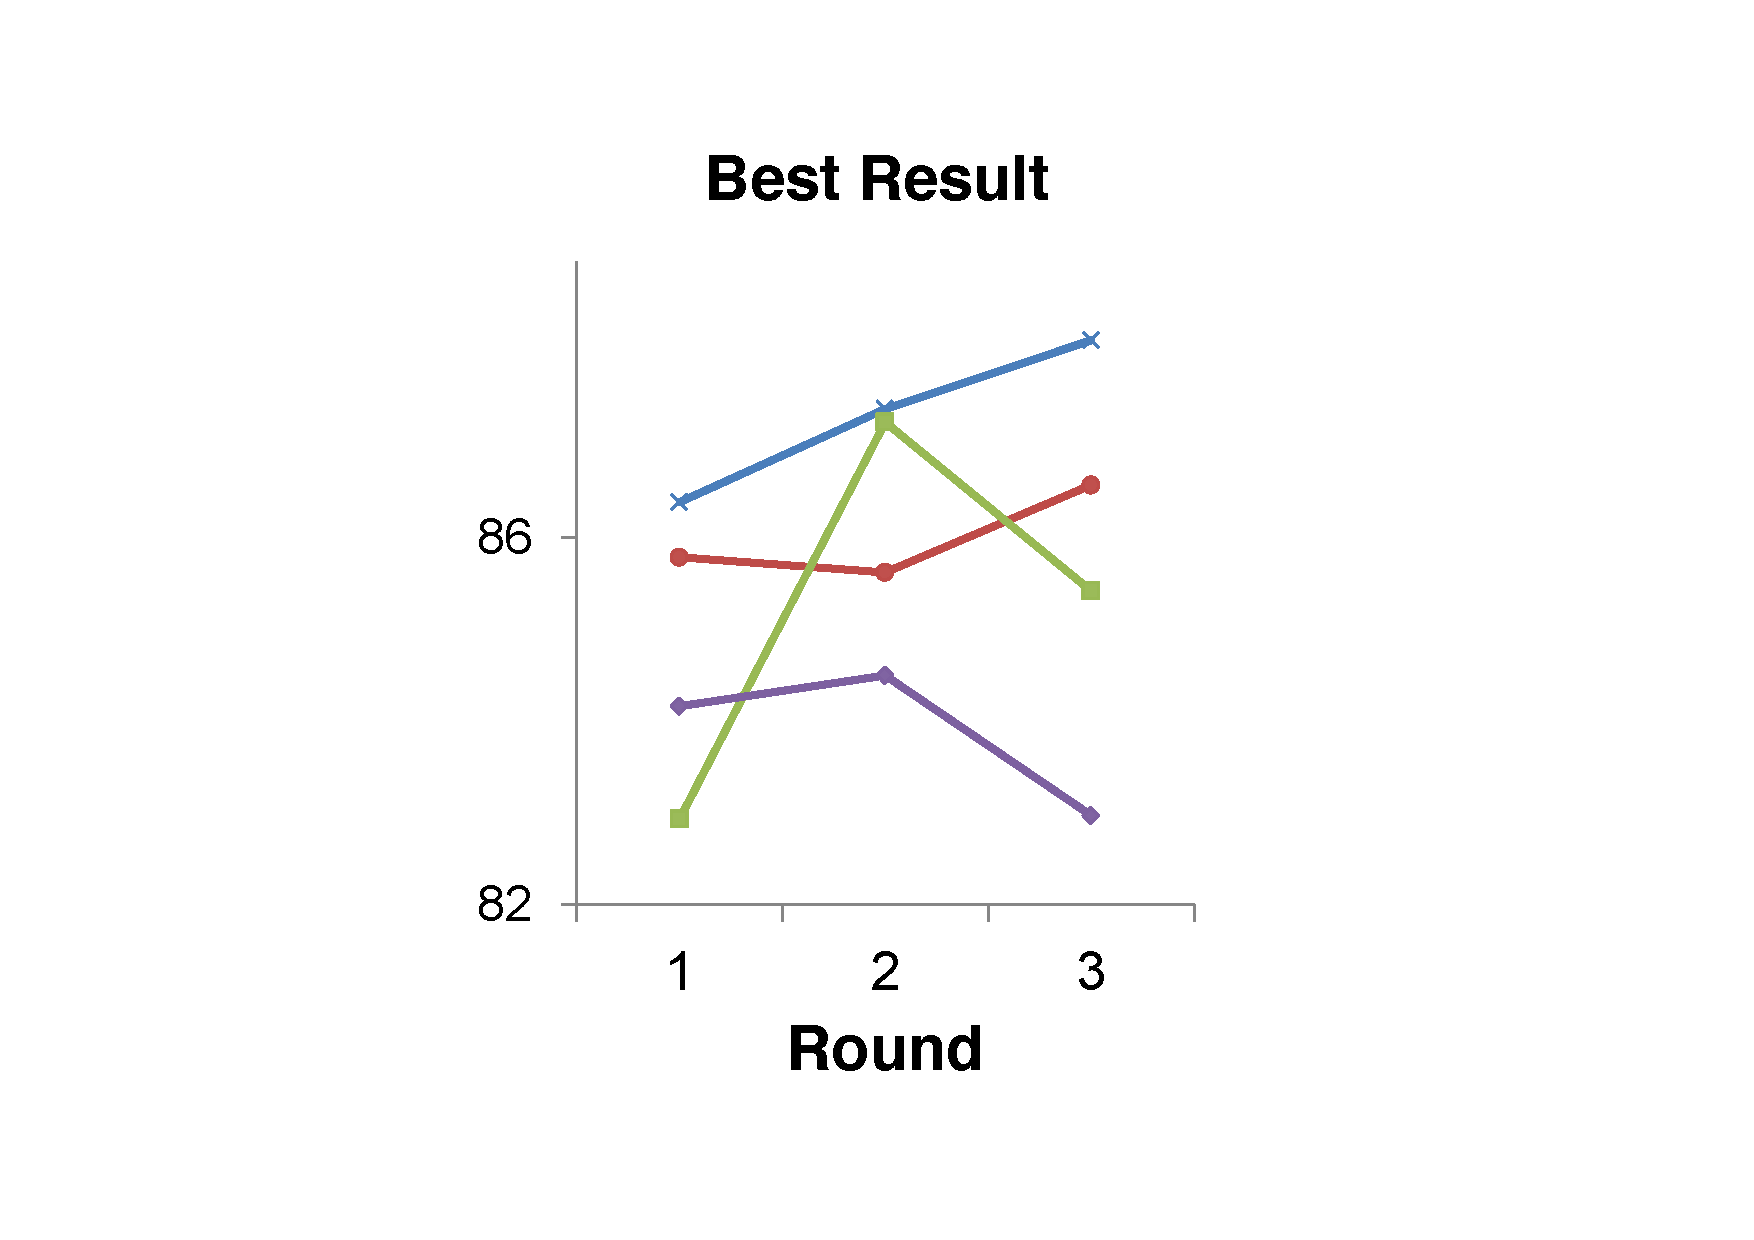
\includegraphics[height = 0.4\textwidth]{PlotBestResult.pdf}
%\end{subfigure}
%\begin{subfigure} 
%\centering
%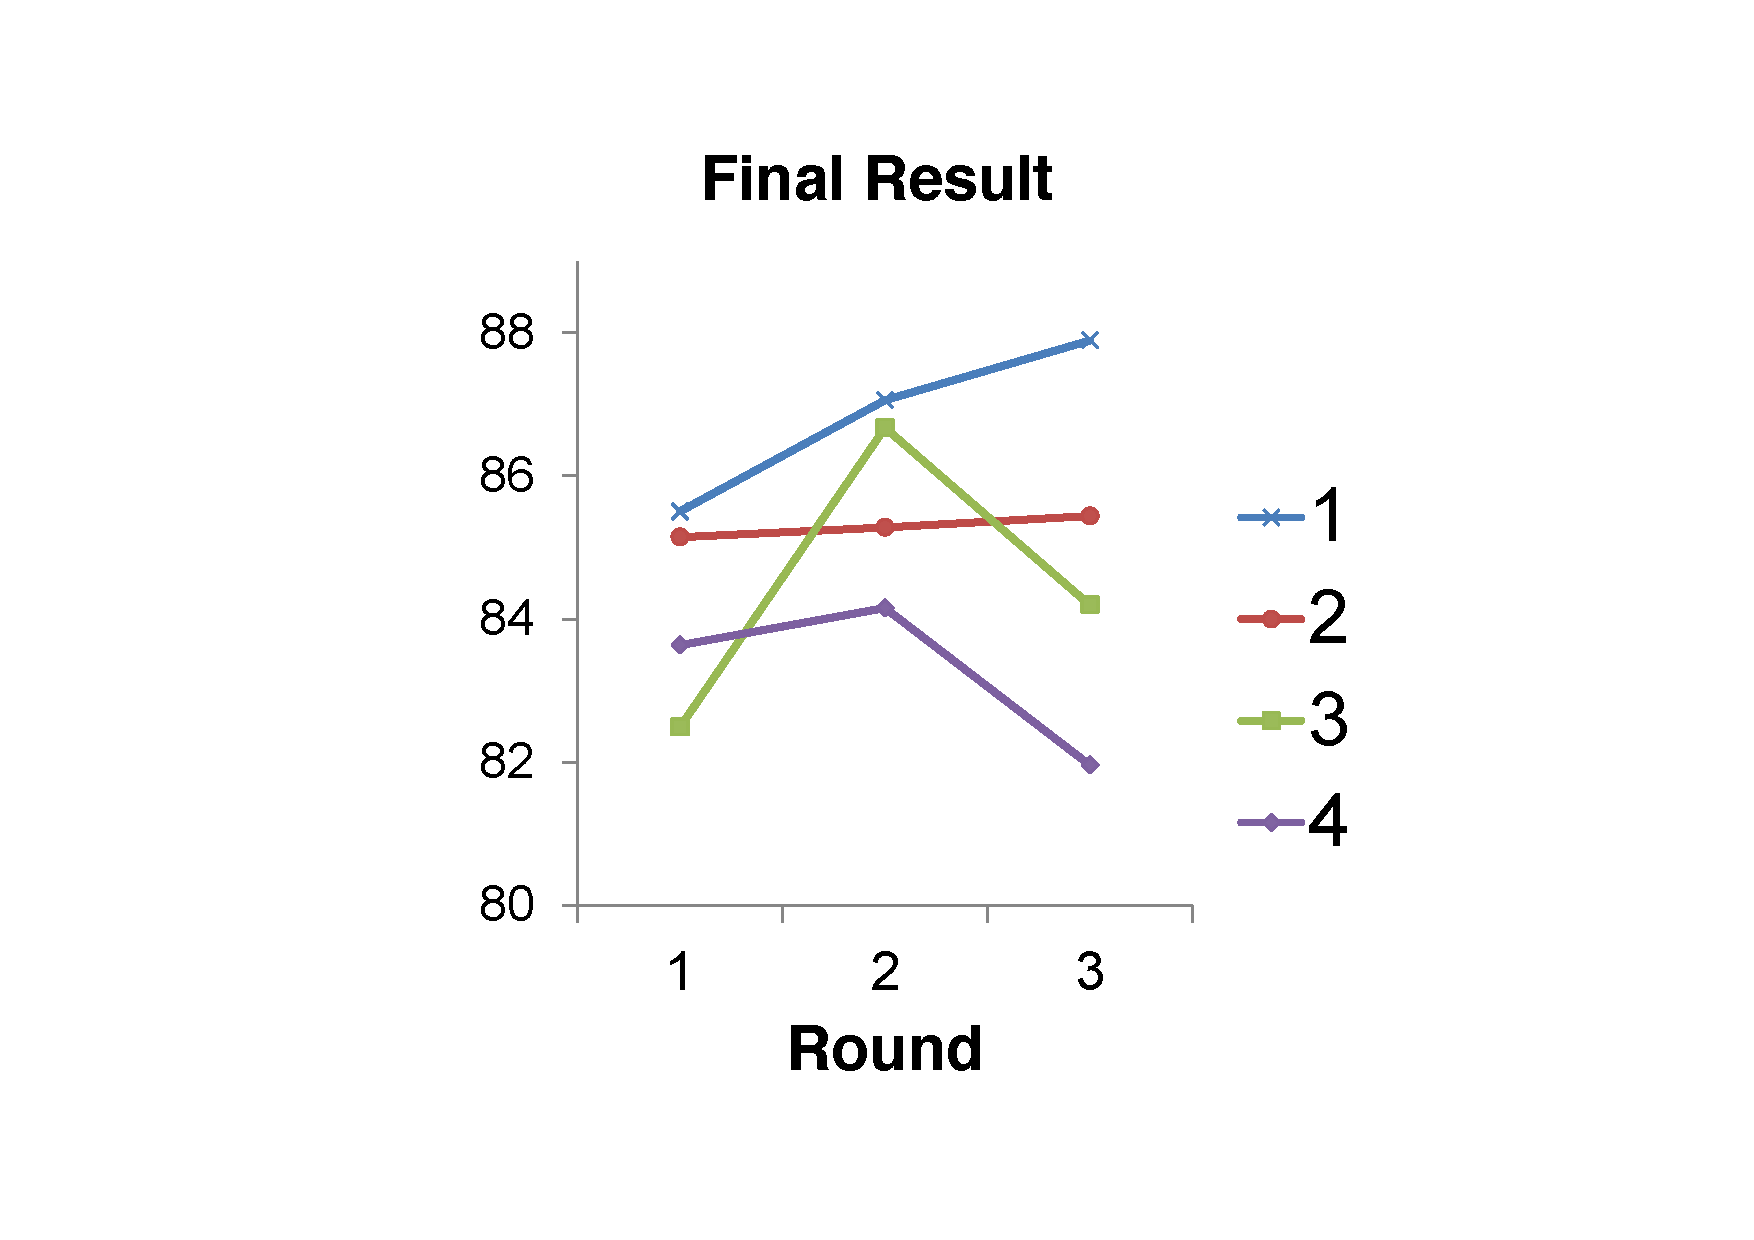
\includegraphics[height = 0.4\textwidth]{PlotFinalResult.pdf}
%\end{subfigure}
% \line(1,0){600}
%
%\begin{subfigure} 
%\centering
%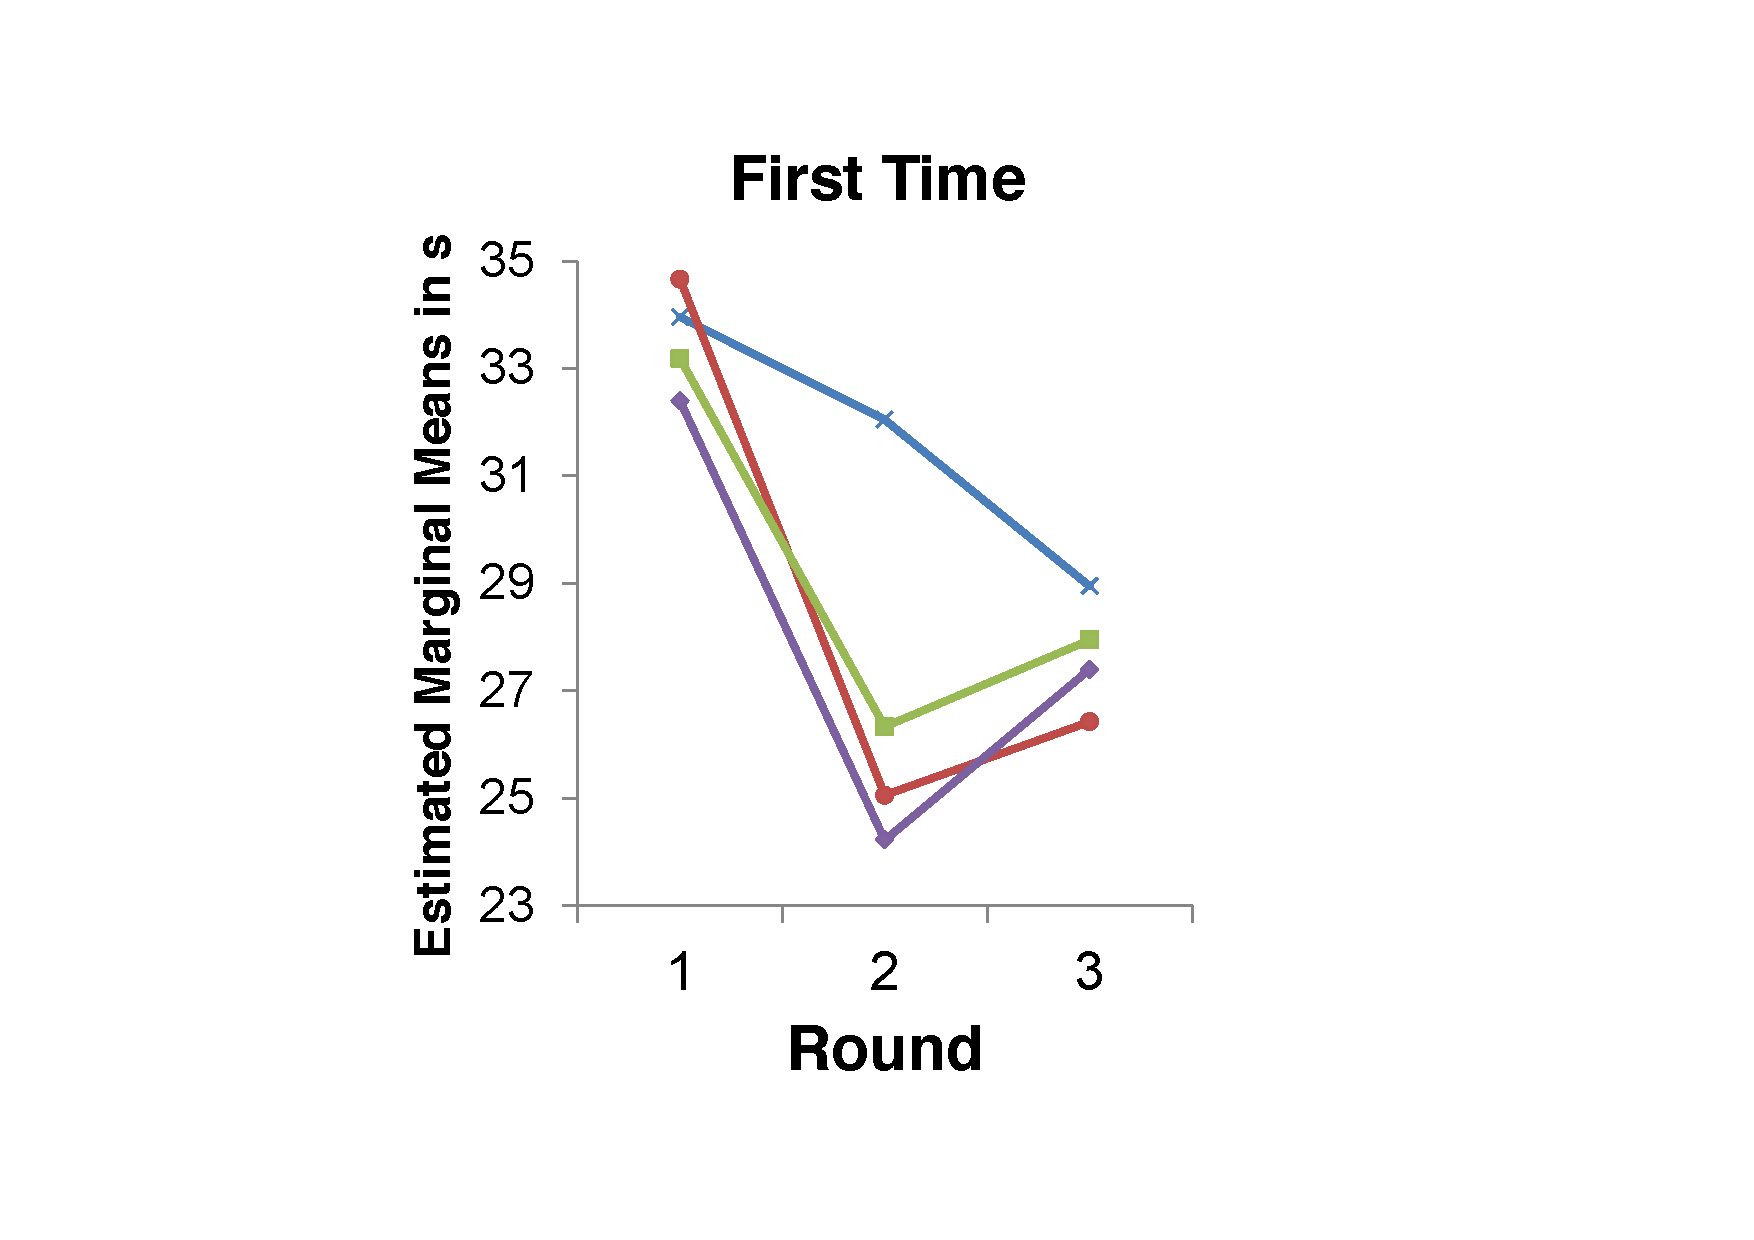
\includegraphics[height = 0.4\textwidth]{PlotFirstTime.pdf}
%\end{subfigure} 
%\begin{subfigure} 
%\centering
%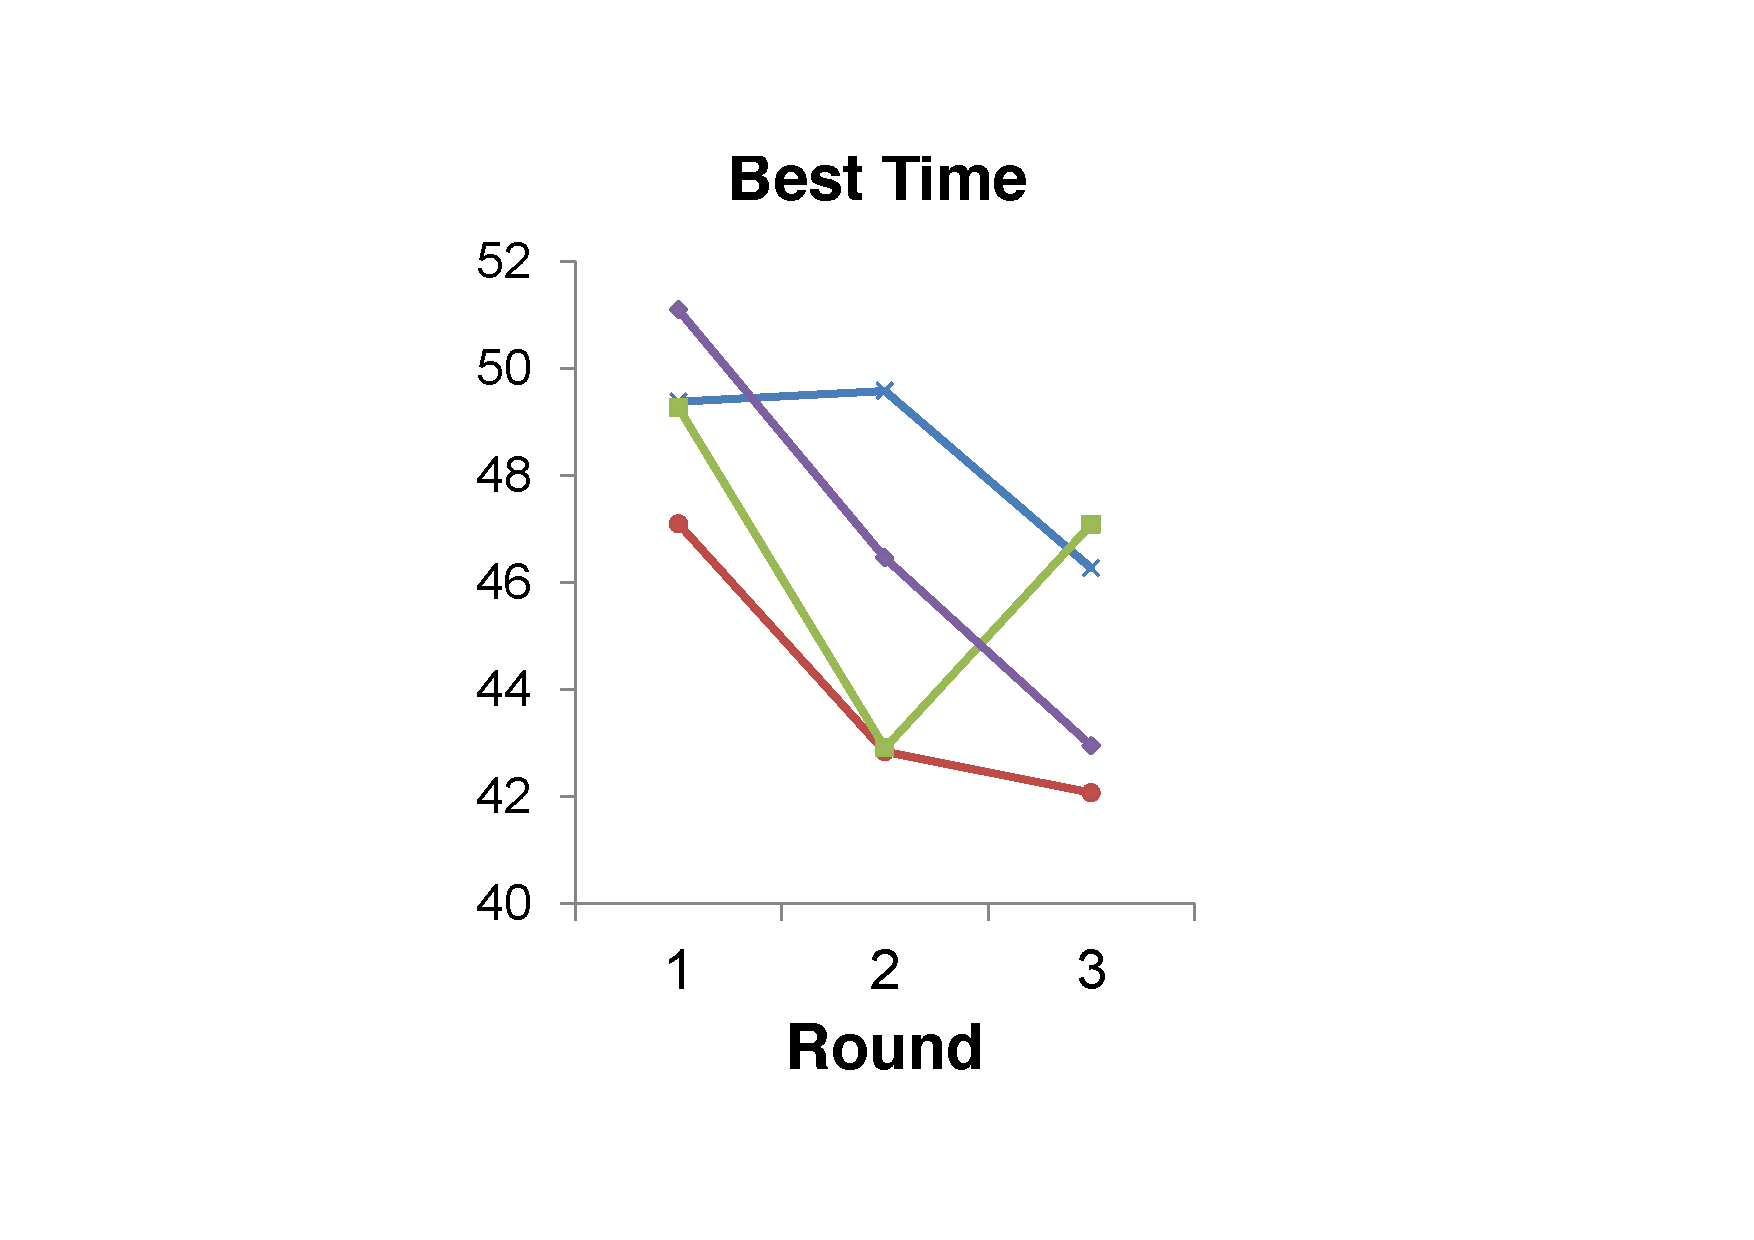
\includegraphics[height = 0.4\textwidth]{PlotBestTime.pdf}
%\end{subfigure}
%\begin{subfigure} 
%\centering
%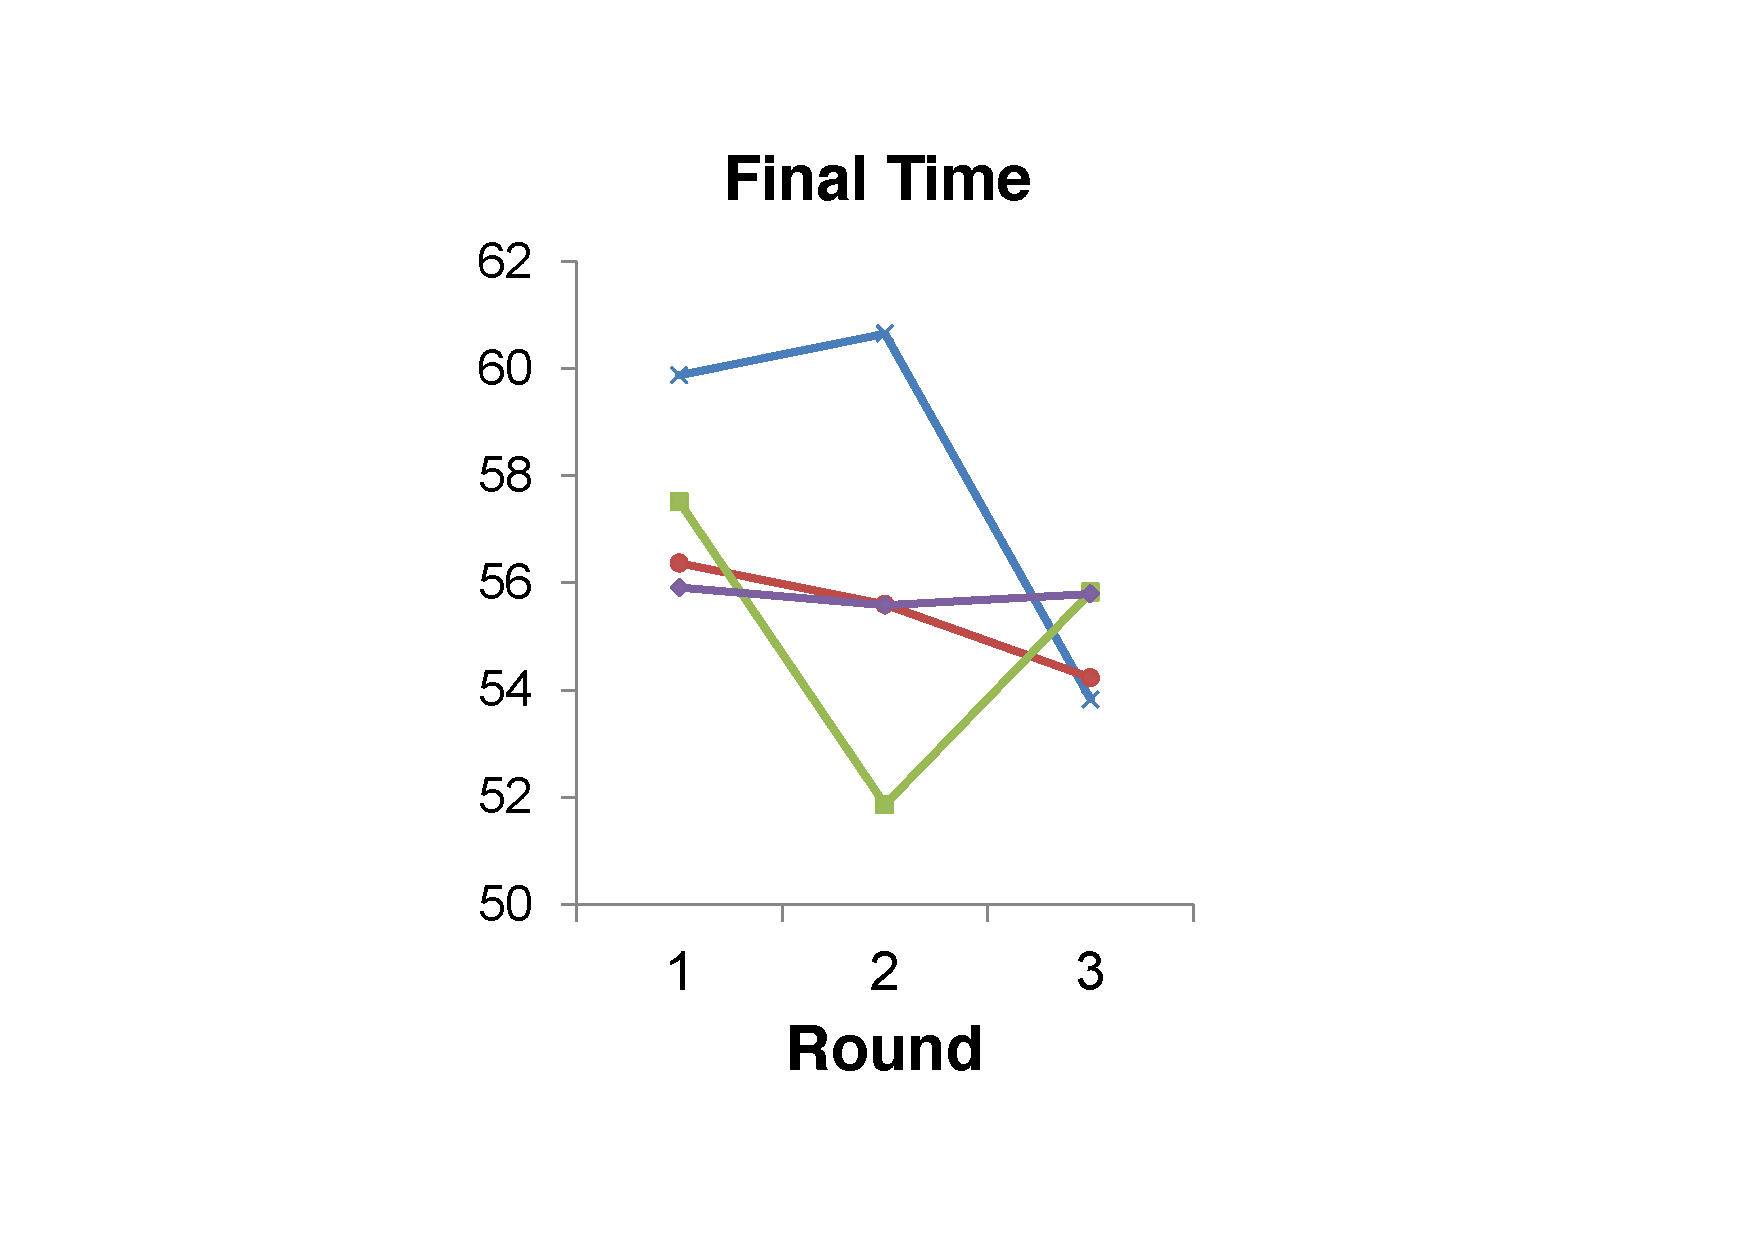
\includegraphics[height = 0.4\textwidth]{PlotFinalTime.pdf}
%\end{subfigure}
%\begin{subfigure} 
%\centering
%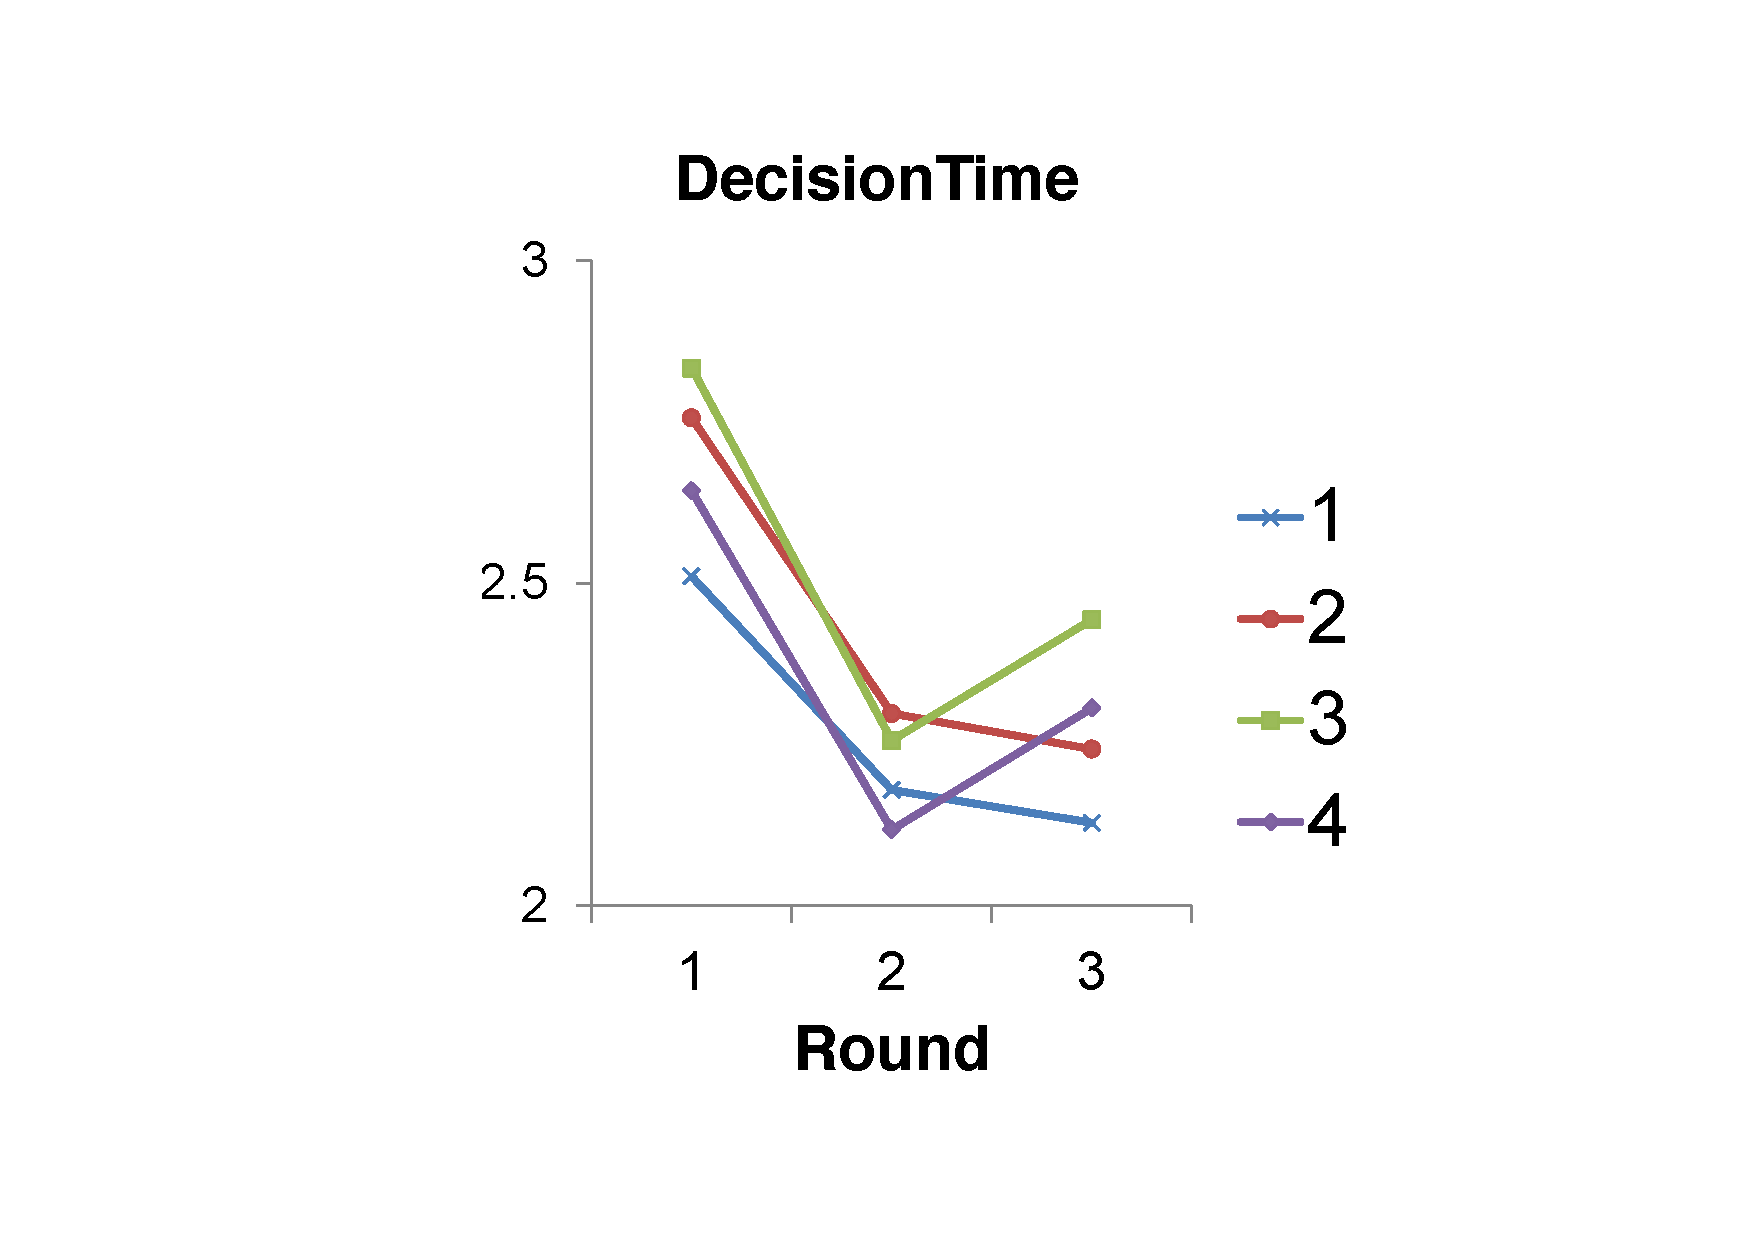
\includegraphics[height = 0.4\textwidth]{PlotDecisionTime.pdf}
%\end{subfigure} 
%\end{flushleft}
%\end{figure}
%\end{landscape}
%}
%\footnotetext{The values for the estimated marginal means are transformed back into the original scale.}
%\subsection{Tests of Between-Subjects Effects: \textit{Usergroup}}
%The estimated marginal means from the \ac{GLM} are displayed in Figure \ref{Estimated Marginal Means over Round for each usergroup}.\\
%For the three results types, Figure \ref{Estimated Marginal Means over Round for each usergroup} shows a clear difference in the results between usergroups 1 and 4, yet usergroups 2 and 3 return mixed results and therefore dilute the validity of the model. For \textit{FirstTime}, usergroups 2, 3 and 4 have very similar values, the variable \textit{BestTime} is noticeable different for usergroup 1 and 2. Usergroups 2 and 3 show similar values for \textit{FinalTime}, the pairs of usergroup 1 and 2, and 3 and 4 have similar trends for \textit{DecisionTime}.\\
%The significance values for the influence of the variable \textit{Usergroup} (Tabel \ref{tab:GLMUsergroup}) do not confirm a general influence on all usergroups, since they are much greater than .05. This leads to the conclusion that the number of colours does not contribute to the model using all usergroups.\\
% If usergroups 2 and 3 are excluded from the data, the influence of \textit{Usergroup} gets significant on the .10 value for all result types. Nevertheless the partial $\eta^2$ remains low. All time variables are not significantly influenced by the usergroups.
%% Table generated by Excel2LaTeX from sheet 'Usergroup'
%\begin{table}[htbp]
%  \centering
%  \caption{GLM - Results for \textit{Usergroup} effect}
%    \label{tab:GLMUsergroup}
%    \begin{tabular}{c||c|c||c|c}
%    \multirow{2}[1]{*}{Variable} & \multicolumn{2}{c||}{No Filter} & \multicolumn{2}{c}{Usergroup 1 and 4} \\
%          & p     & $\eta_{partial}^2$ & p & $\eta_{partial}^2$ \bigstrut[b]\\
%    \hline
%    \textit{First Result} & ns    & -   & $\cdot$    & .04 \bigstrut\\
%    \hline
%    \textit{BestResult} & ns    & -   & $\cdot$     & .03 \bigstrut\\
%    \hline
%    \textit{FinalResult} & ns    &  -  & $\cdot$     & .03 \bigstrut\\
%    \hline
%    \multicolumn{5}{c}{\textit{ns: FirstTime, BestTime, FinalTime, DecisionTime}} \bigstrut[t]\\
%    \end{tabular}%
%\end{table}%
%		
%\subsection{Tests of Within-Subjects Effects: \textit{Round}}
%As indicated by Figure \ref{Estimated Marginal Means over Round for each usergroup}, the \textit{Round} influence seems to be positive for usergroup 1, yet usergroups 2, 3 and 4 do not return distinct results. No overall monotonous effect from \textit{Round} on the times can be detected in the graphs, however there seems to be a noticeable influence from round 1 to 2 on \textit{FirstTime}, \textit{BestTime} and \textit{DecisionTime}.
%
%A Univariate Test, using the Greenhouse-Geisser, Huynh-Feldt and Lower-bound tests\footnote{The Sphericity Assumed
%test is not included since the covariance matrix assumption is not met.}, confirms that for \textit{BestResult}, \textit{FinalResult}, \textit{FirstTime}, \textit{BestTime} and \textit{DecisionTime} the within-subjects effects contribute to the model (Tabel \ref{tab:GLMRound}). No significant results are found for the \textit{FirstResult} and \textit{FinalTime}. Nevertheless the values for the $\eta_{partial}^2$ are very small (< .1), so the \textit{Round} effect only explains a small portion of the variation in the outcome of the majority of the variables. The $\eta_{partial}^2$ for \textit{DecisionTime},however, has a higher value.
%% Table generated by Excel2LaTeX from sheet 'Round'
%\begin{table}[htbp]
%  \centering
%  \caption[GLM - Results for Round effect]{GLM - Results for \textit{Round} effect\footnotemark}
%    \label{tab:GLMRound}
%    \begin{tabular}{c|c|c|c|c|c|c}
%    \multirow{2}[1]{*}{Variable} & \multicolumn{2}{c|}{No Filter} & \multicolumn{2}{c|}{Usergroup 1 \& 4} & \multicolumn{2}{c}{Round 1 \& 2} \\
%          & p     & $\eta_{partial}^2$ & p     & $\eta_{partial}^2$ & p     & $\eta_{partial}^2$ \bigstrut[b]\\
%    \hline
%    \textit{BestResult} & $\cdot$     & .02 & ns    & -     & *    & .03 \bigstrut[t]\\
%    \hline
%    \textit{FinalResult} & $\cdot$     & .02 & ns    & -     & *    & .03 \bigstrut[b]\\
%    \hline
%    \textit{FirstTime} & *    & .08   & *    & .05   & **   & .13 \bigstrut\\
%    \hline
%    \textit{BestTime} & *    & .03   & $\cdot$     & .03   & *    & .03 \bigstrut\\
%    \hline
%    \textit{DecisionTime} & *    & .19   & **   & .16   & **   & .27 \bigstrut[t]\\
%    \multicolumn{7}{c}{\textit{ns: FirstResult, FinalTime}} \\
%    \end{tabular}%
%\end{table}%
%\footnotetext{Greenhouse-Geisser, Huynh-Feldt, Lower-bound statistics aggregated.}
%
%The graphical assumption for usergroup 1 - a potential influence from \textit{Round} on the three result types - is not acknowledged by the results from the tests. Looking at the specific \textit{Round} level, the contrast results indicate that the \textit{Round} influence is significant for the 1\textsuperscript{st} to the 2\textsuperscript{nd} round for all the displayed variables in the table (p < .05).\\
%%% Table generated by Excel2LaTeX from sheet 'Latex'
%%\begin{table}[htbp]
%%  \centering
%%  \caption[GLM - Results for the different effects]{\ac{GLM} - Results for the different effects\footnotemark}
%%    \label{GLM - Results for the different effects}%
%%    \begin{tabular}{c|c||c|c||c|c||c|c}
%%    \multirow{2}[1]{*}{Effect} & \multirow{2}[1]{*}{Variable} & \multicolumn{2}{c||}{No Filter} & \multicolumn{2}{c||}{Usergroup 1 \& 4} & \multicolumn{2}{c}{Round 1 \& 2} \\
%%          &       & p     & partial $\eta^2$ & p     & partial $\eta^2$ & p     & partial $\eta^2$ \bigstrut[b]\\
%%    \hline
%%    \multirow{3}[6]{*}{Usergroup} & \textit{FirstResult} & .41  & .02  & \cellcolor{darkgrey}.04  & \cellcolor{grey}.04  & -     & - \bigstrut\\
%%\cline{2-8}          & \textit{BestResult} & .58  & .01  & \cellcolor{darkgrey}.10  & \cellcolor{grey}.03  & -     & - \bigstrut\\
%%\cline{2-8}          & \textit{FinalResult} & .56  & .01  & \cellcolor{darkgrey}.10  & \cellcolor{grey}.03  & -     & - \bigstrut\\
%%    \hline
%%    \multirow{3}[6]{*}{Round\footnotemark} & \textit{FirstResult} & >  .5 & < .01 & >  .9 & < .01 & >  .9  & < .01 \bigstrut\\
%%\cline{2-8}          & \textit{BestResult} & \cellcolor{darkgrey}<  .1 & < \cellcolor{grey}.02 & >  .6 & < .01 & \cellcolor{darkgrey}.03  & \cellcolor{grey}.03 \bigstrut\\
%%\cline{2-8}          & FinalResult & \cellcolor{darkgrey}<  .1 & \cellcolor{grey}< .02 & >  .3 & < .01 & \cellcolor{darkgrey}.01  & \cellcolor{grey}.03 \bigstrut\\
%%    \hline
%%    Usergroup & \textit{FirstResult} & >  .2 & < .01 & .14  & .02  & \cellcolor{darkgrey}.04  & \cellcolor{grey}.05 \bigstrut\\
%%\cline{2-8}    *     & \textit{BestResult} & \cellcolor{darkgrey}<  .1 & \cellcolor{grey}< .02 & .59  & < .01  & \cellcolor{darkgrey}.06  & \cellcolor{grey}.04 \bigstrut\\
%%\cline{2-8}    Round\footnotemark & \textit{FinalResult} & \cellcolor{darkgrey}<  .1 & \cellcolor{grey}< .03 & .46  & .01  & .14  & .03 \bigstrut[t]\\
%%    \end{tabular}%
%%\end{table}%
%%\footnotetext{Significance level is .10. Cases with rejected hypothesis are marked in dark grey, the corresponding partial $\eta^2$ in grey.}
%%\footnotetext{Greenhouse-Geisser, Huynh-Feldt, Lower-bound statistics aggregated.}
%
%\subsection{Tests of a combination of Within-Subjects Effects and Between-Subjects Effects}
%The univariate test combining the contribution of \textit{Usergroup} and \textit{Round} indicates a minor influence of the combined variables on \textit{BestResult} and \textit{FinalResult} with all statistics showing significant values on the .10 level (Table \ref{tab:GLMUsergroupRound}). This is most likely caused by the significant individual influence from \textit{Round}.
%On the specific \textit{Round} level, however, one can also find a significant contribution from Round 1 to Round 2 on the \textit{FirstResult}, yet the $\eta_{partial}^2$ is again very low. These findings are rather suspect, since there is no significant influence from each individual variable detectable for the \textit{FirstResult}.
%For the time variables, no significant influence by a combination between \textit{Usergroup} and \textit{Round} can be detected.
%% Table generated by Excel2LaTeX from sheet 'UsergroupRound'
%\begin{table}[htbp]
%  \centering
%  \caption[GLM - Results for Usergroup \& Round effect]{GLM - Results for \textit{Usergroup} \& \textit{Round} effect\footnotemark}
%    \label{tab:GLMUsergroupRound}
%    \begin{tabular}{c||c|c||c|c||c|c}
%    \multirow{2}[1]{*}{Variable} & \multicolumn{2}{c||}{No Filter} & \multicolumn{2}{c||}{Usergroup 1 \& 4} & \multicolumn{2}{c}{Round 1 \& 2} \\
%          & p     & $\eta_{partial}^2$ & p     & $\eta_{partial}^2$ & p     & $\eta_{partial}^2$ \bigstrut[b]\\
%    \hline
%    \textit{First Result} & ns    & -     & ns    & .02   & *    & .05 \bigstrut\\
%    \hline
%    \textit{BestResult} & $\cdot$     & .02   & ns    & .00   & $\cdot$     & .04 \bigstrut\\
%    \hline
%    \textit{FinalResult} & $\cdot$     & .03   & ns    & .01   & ns    & - \bigstrut[t]\\
%    \multicolumn{7}{c}{\textit{ns: FirstTime, BestTime, FinalTime, DecisionTime}} \\
%    \end{tabular}%
%\end{table}%
%\footnotetext{Greenhouse-Geisser, Huynh-Feldt, Lower-bound statistics aggregated.}
%
%We conclude that even tough the tests partly return significant values for the mutual influence by \textit{Usergroup} and \textit{Round}, these variables only explain a small portion of the values for the result types, since the partial $\eta_{partial}^2$ is very low.
%
%% ===============================
\section{\acf{NP}}
\label{ch:Evaluation:sec:Non-parametrictest}
%% ===============================

\acl{NP}s are statistical models that do not specify restrictive conditions \citep{Siegel1957}, thus \ac{NP} only make minimal assumptions regarding the underlying distribution of the data. Their advantages include the fact that the data does not have to be normally distributed. Furthermore, the tests rank the values instead of looking at the values themselves which makes them robust against outliers.\\
Two different categories of tests are used; an independent-samples test, analysing the dependent variables that are grouped by \textit{NumberOfColours} and \textit{Trial}; and a test for related samples, comparing \textit{Rounds} for the same set of users. 

\subsection{Tests of Independent samples: \textit{NumberOfColours} \& \textit{Trial}}
Two tests are conducted for the independent samples. The Kruskal-Wallis Test of Independent Samples\footnote{For the SPSS source code of the two tests, refer to this \href{http://publib.boulder.ibm.com/infocenter/spssstat/v20r0m0/topic/com.ibm.spss.statistics.help/alg_nonparametric_independent_wald-wolfowitz.htm}{Link}.}, comparing the distributions per \textit{NumberOfColours}, as well as the Mann-Whitney Test, which compares the two \textit{Trials} against each other.\\
Null and alternative hypotheses are defined in the following way: 

\textbf{Kruskal-Wallis- \& Mann-Whitney-Test} \\
\textbf{H\textsubscript{0}:} \textit{The distribution of the dependent variables are the same across different usergroups.}\\
\textbf{H\textsubscript{A}:} \textit{At least one distribution is different.}

\paragraph{\textit{Trial}}
The Mann-Whitney-Test retains the null hypothesis for all dependent variables for the influence of \textit{Trial} (Table \ref{NPTest}), so the different bonus systems do not seem to have an influence on the outcomes in the data.

\paragraph{\textit{NumberOfColours}}
The results for the Kruskal-Wallis-Test are dependent on the applied filters (Table \ref{NPTest}). Except of \textit{DecisionTime}, there is no influence of the \textit{NumberOfColours} detectable for the unfiltered data, yet there is an undefined, but detectable influence for Filter 1. Kruskal-Wallis-Test for Filter 2 shows an influence for the result variables.
\textit{FirstTime} only seems to be affected by the \textit{Round} due to the retention of the null hypothesis for the \textit{NumberOfColours}. 
% Table generated by Excel2LaTeX from sheet 'NumberOfColours'
\begin{table}[htbp]
  \centering
  \caption{Results for the NP Independent \& Dependent Tests}
    \label{Results for the NP Test}
    \begin{tabular}{c|c|ccc|c}
    \toprule
       Reject   & \textit{Trial} & \multicolumn{3}{c|}{\textit{NumberOfColours}} & \textit{Round} \\
       hypotheses  & Any Filter & Unfiltered & Filter 1 & \multicolumn{1}{c|}{Filter 2} & Any Filter \\
    \midrule
	\textit{FirstResult} & &              & $\surd$     & $\surd$     &  $\surd$ \\
    \textit{BestResult} & &         	  & $\surd$     & $\surd$	   & $\surd$\\
    \textit{FinalResult} & &         	  & $\surd$ 	 & $\surd$	   & $\surd$ \\
    \textit{FirstTime} & &         		  &       		 &       	   & $\surd$ \\
    \textit{BestTime} & &         		  & $\surd$     &              & $\surd$ \\
    \textit{FinalTime} & &         		  & $\surd$     &              & $\surd$ \\
    \textit{DecisionTime} & &  $\surd$    & $\surd$     &       	   & $\surd$ \\
    \textit{DecisionNumber} & &           & $\surd$     &       	   & $\surd$ \\
    \bottomrule
    \end{tabular}%
  \label{NPTest}%
\end{table}%

%Table \ref{Results for the NP Independent Test} shows the result for each result type and test.
%For the unfiltered data, only the median test for \textit{FirstResult} rejects the null hypothesis and indicates a significant median difference between  usergroup 1 and 4 (Figure \ref{fig:NPFirstResultBoxplot}). Interestingly, the Kruskal-Wallis test for the same variable retains the null hypothesis with a high p-value.\\
%The results are further evaluated by filtering the data to only include usergroups 1 and 4. The findings of the Mann-Whitney-Test get clearer for all result variables, the null hypotheses can be rejected for a p-value of .10. No significant results are returned for all time variables\\
%We conclude that there are statistically significant differences between usergroups 1 and 4 for the result variables, but there are no significant findings when looking at all usergroups.\\
%\begin{figure}[htbp] % NPFirstResultBoxplot	
%\begin{center} 
%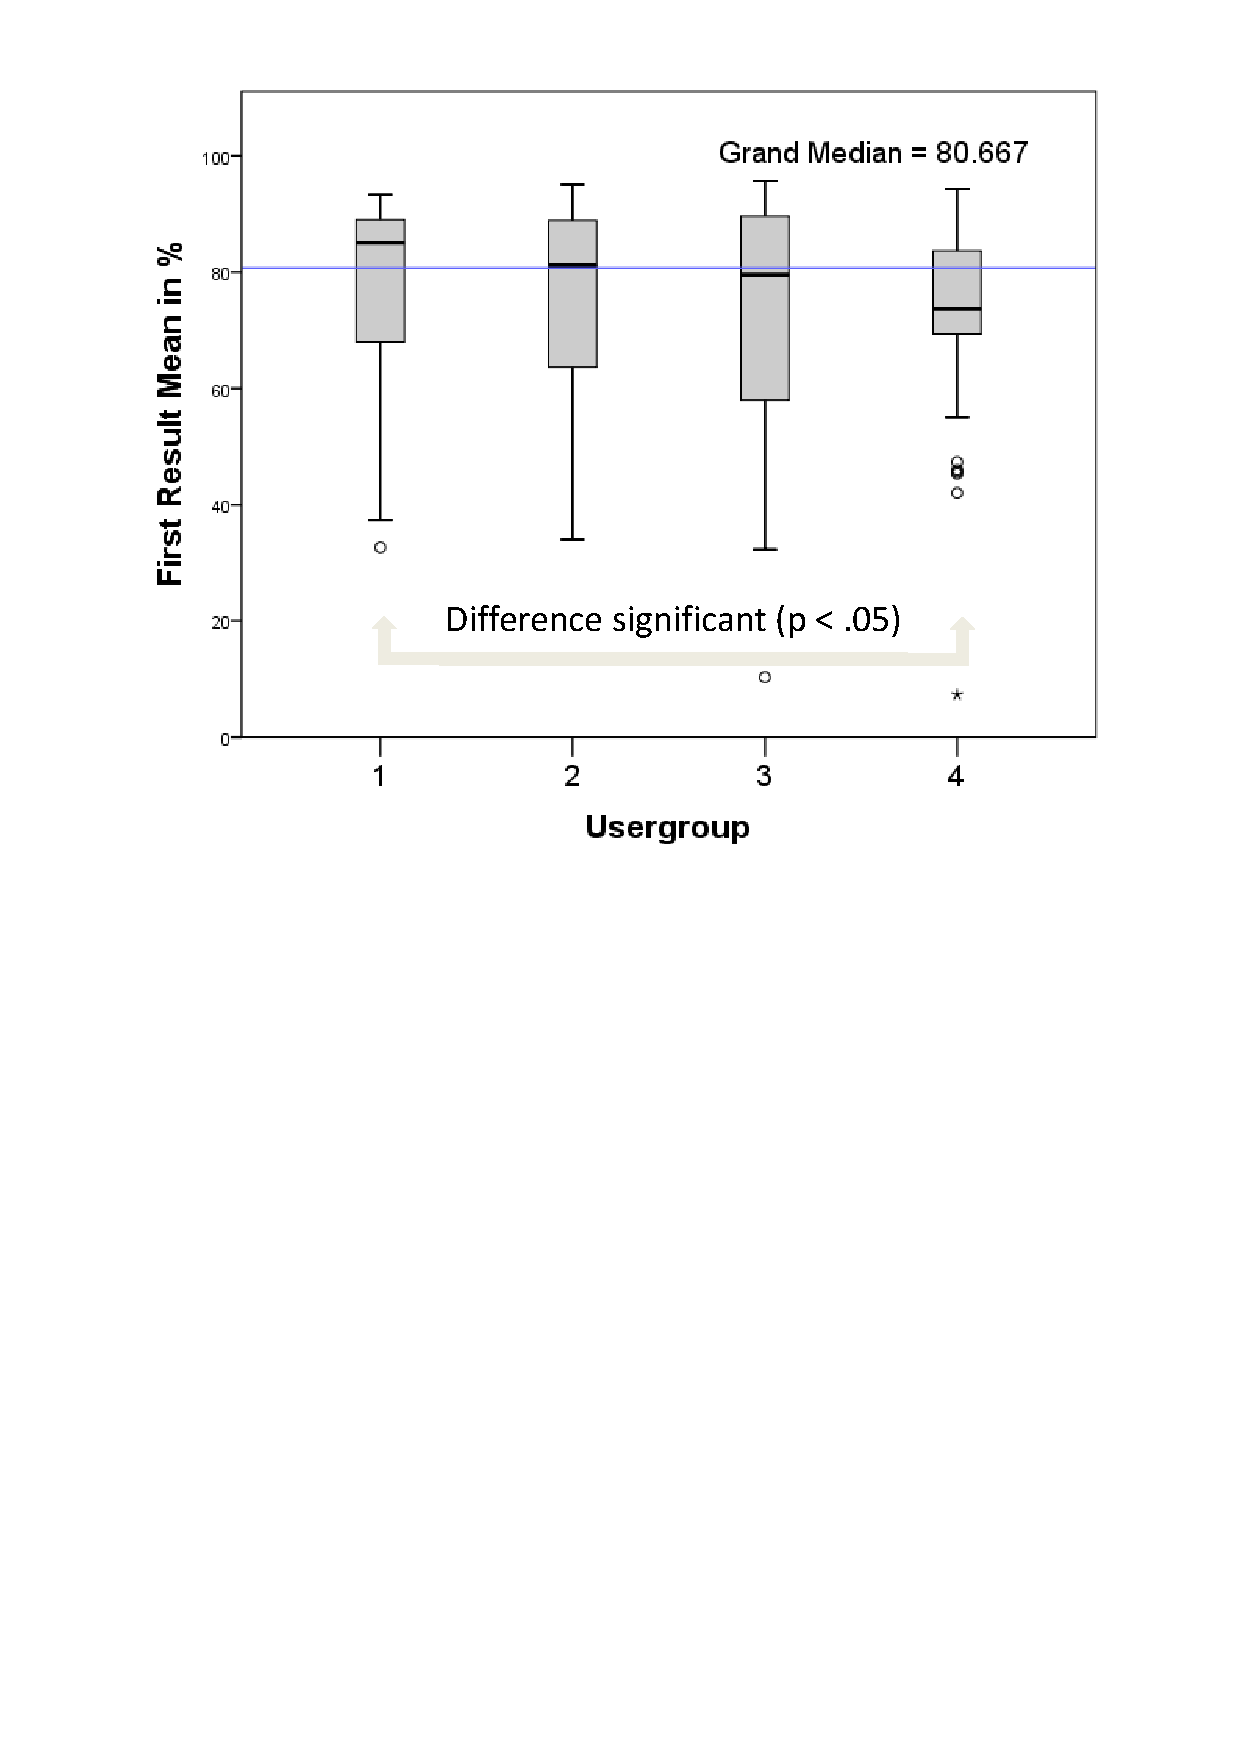
\includegraphics[height = 0.5\textwidth]{NPFirstResultBoxplot.pdf}
%  \caption{Boxplot for FirstResult with Grand Median}
%    \label{fig:NPFirstResultBoxplot} 
%\end{center}
%\end{figure}

\subsection{Tests of dependent samples: \textit{Round}}
A related-Samples Friedman's Two-Way Analysis of Variance by Ranks test \citep{Friedman1937} is applied to compare the values in-between \textit{Rounds}. The null and alternative hypotheses are defined in the following way:

\textbf{Friedman's Test} \\ 
\textbf{H\textsubscript{0}:} \textit{The distributions of the dependent variables are the same across rounds.}\\
\textbf{H\textsubscript{A}:} \textit{At least one distribution is different.}

Friedman's Test results are shown in Table \ref{NPTest} and reject the null hypothesis for all dependent variables. The applied filter does not have an influence on the findings.

\subsection{Conclusion}
The findings for the \ac{NP} tests underline the magnitude of the statistical noise in the unfiltered data. According to the Kruskal-Wallis-Test, no influence is detectable by \textit{NumberOfColours} when no filter is used. As a result, a parameter estimation is only suitable for Filter 1 and Filter 2.\\
Furthermore, not every dependent variable seems to be influenced by the independent variables for the filtered data, so the parameter estimations for those variables might be non-significant.
\newpage
%% ===============================
\section{\acf{LMM}}
\label{ch:Evaluation:sec:LMM}
%% ===============================

%The results from the \ac{LMM} and the \ac{NP}s do not confirm the majority of the hypothesis. In fact, the findings have not confirmed an influence of \textit{Round} and \textit{NumberOfColours}, so one would assume that providing parameter estimates will not introduce further significant findings as well.\\
For the purposes of testing the proposed polynomial relationship between the dependent variables and the \textit{NumberOfColours} as well as the logarithmic influence of \textit{Round}, we examine the data using a \acl{LMM}. This model is a powerful modelling tool that allows the analysis of complex datasets with hierarchical structures \citep{Galecki2013}. As a result, the \acl{LMM} is an appropriate choice with a high power-efficiency for the conditions of our research.

The term \textit{Mixed Model} refers to the use of both fixed and random effects in the same analysis \citep{Seltman2012}. Whereas fixed effects are essential to evaluate the potential polynomial relationship between the independent and dependent variables, random effects aggregate the influences which are not relevant for the purposes of this study. \\ 
Fixed effects are usually related to treatments (\textit{NumberOfColours} and \textit{Trial}), whereas subject effects are defined as random effects (\textit{User}).\\
Subject effects include the individual characteristics of each participant. These effects (e.g. experience with similar tasks or the general ability to perform well in the given task), have an influence on the result and time variables, but are not the focus of our research. As described in Section \ref{ch:Experiment:sec:OnlineImplementation}, one implication for cognitive load experiments on \acf{AMT} is the lack of control over what participants are doing during the experiment. By taking into account these individual influences, and separating them from the focus of the research, the noise of the data can be reduced and can return more significant results.

\paragraph{Normality Assumption}
The normality assumption is not met by the original data, so a data transformation is necessary.
We use the Box-Cox transformation\footnote{See Equation \ref{BoxCoxTransformation} in Appendix \ref{Appendix-Formulas} for the formula.} \citep{Sakia1992} that applies a shifted power transformation to adjust the standard deviation and the mean to the requested values for the normal distribution. Since the method is using a range of power transformations, the efficiency of normalizing and variance equalizing for both positively- and negatively-skewed variables can be improved \citep{Osborne2010}. In order to find the optimal input parameter $\lambda$ for the transformation, we implement Osborne's SPSS algorithm. \\
We find suitable $\lambda$-values for the variables \textit{FirstTime} and \textit{DecisionTime}. Nevertheless, no adequate values can be found for all result types, namely \textit{BestTime}, \textit{FinalTime} and \textit{DecisionNumber}.
Figure \ref{fig:SkewKurtosis} provides an explanation for the lack of appropriate $\lambda$-values in the \textit{FirstResult}. No $\lambda$-values can be found that reduce the skewness and kurtosis of the transformed data to a limit at which one can assume a normal distribution. Similar results are returned for \textit{BestResult}, \textit{FinalResult}, \textit{BestTime} and \textit{FinalTime}.
\begin{figure}[htbp] % Transformation	
\begin{center} 
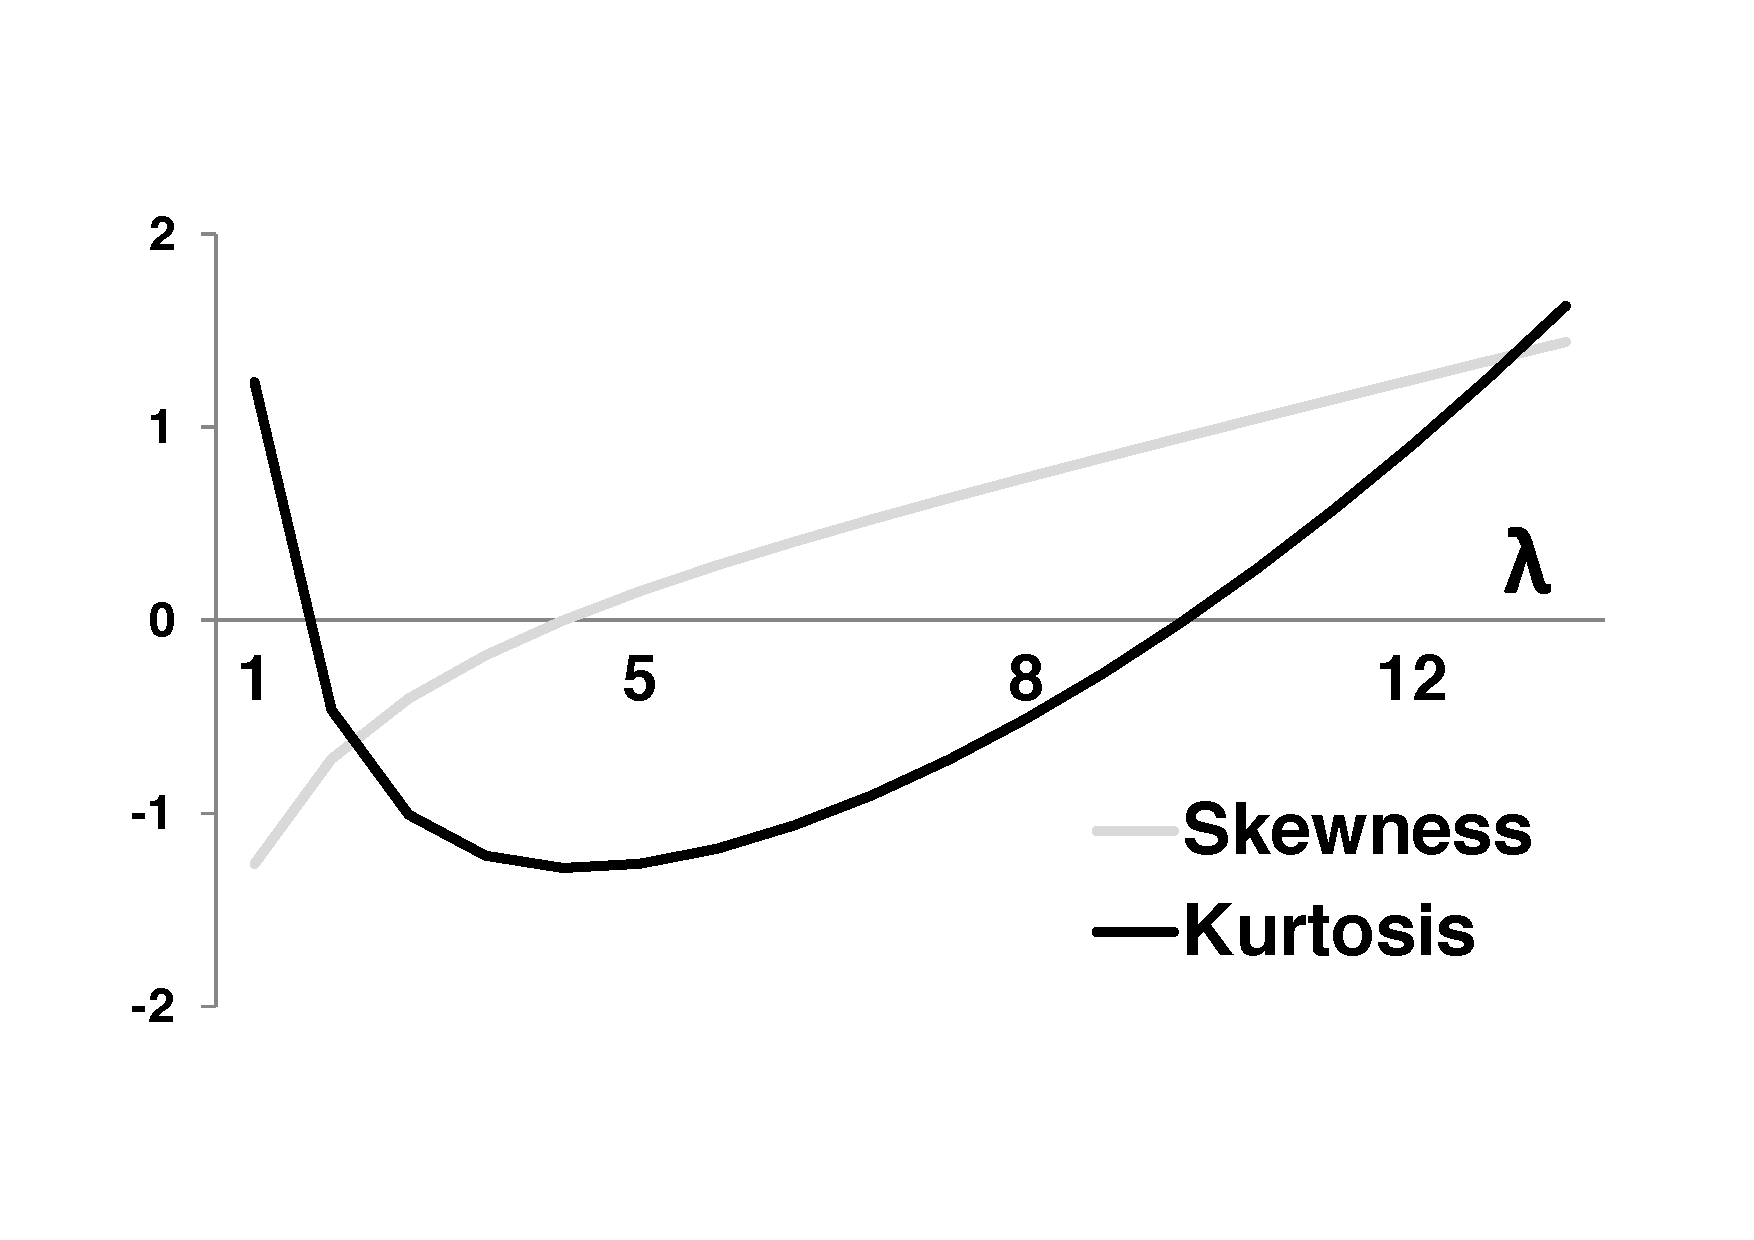
\includegraphics[height = 0.30\textwidth]{SkewKurtosis.pdf}
  \caption{Transformation \textit{FirstResult} - Skewness and Kurtosis for different $\lambda$ values}
    \label{fig:SkewKurtosis} 
\end{center}
\end{figure}
In addition, a test of Normality proves our previous findings that a Box-Cox-transformation is only suitable for \textit{FirstTime} and \textit{DecisionTime}. Since we have a data set smaller than 2000 elements, the Shapiro-Wilk test \citep{Shapiro1965} is used to test the null hypothesis which states that the observed population does not come from a normal distribution. The p-value is greater than 0.05 only for \textit{FirstTime} and \textit{DecisionTime}, so we must retain the null hypothesis for all other variables and conclude that only the data transformation of \textit{FirstTime} and \textit{DecisionTime} comes from a normal distribution.

%\textbf{2. Constant covariance matrix: \makebox[0pt][l]{$\square$}\raisebox{.15ex}{\hspace{0.1em}{\color{red}x}}}\\
%The Box's M test statistic \citep{Box1949} conducted on SPSS tests the null hypothesis that the observed covariance matrices of the dependent variables are not equal across groups. The significance value of the test is less than .10, suggesting that the assumptions are not met and the covariance matrix does differ across usergroups.\\
%\textbf{3. Equal Error variance: \makebox[0pt][l]{$\square$}\raisebox{.15ex}{\hspace{0.1em}{\color{green}$\checkmark$}}}\\ 
%The \cite{Levene1960}'s Test of Equality of Error Variances tests the null hypothesis that the error variance of the dependent variable is not equal across groups.
%The test shows no significant value for the majority of the variables on the .10 significance level and is not significant on the .05 level for two variables. As a result, the null hypothesis can be rejected and we can assume that the equal variances assumption is not violated for each variable.
\paragraph{Conclusion}
The validity of the results based on the \ac{LMM} depends on whether or not its conditions are met \citep{Siegel1957}. Since the normality assumption is not fulfilled for the majority of the variables, the addressed power of the \ac{LMM} might be diluted. \\
According to \cite{Graybill1976}, we can either ignore the violation of the assumptions and proceed with the analysis as if all assumptions were satisfied, or we can use a distribution-free procedure. \\
A distribution-free procedure in the form of non-parametric tests is used in Section \ref{ch:Evaluation:sec:Non-parametrictest}. Yet, these tests do not give information about potential parameter estimations for an implemented model.
Therefore, we continue analysing the data using the \ac{LMM}.

\subsection{Choice of a \ac{LMM} model}
Specifying a mixed model requires several steps, each of which requires an informed decision \citep{Seltman2012}. \\
First, the identification of  fixed effects requires the specification of which influences affect the average performances for all individuals.  We assume that the level of \textit{NumberOfColours} and the \textit{Round} number affects each participant.
The \acl{NP} in Section \ref{ch:Evaluation:sec:Non-parametrictest} do not show any significant influence on the population mean from the \textit{Trial}, so we do not take this variable into consideration as a fixed effect.\\
\begin{figure}[htbp] % RandomIntercept	
\begin{center} 
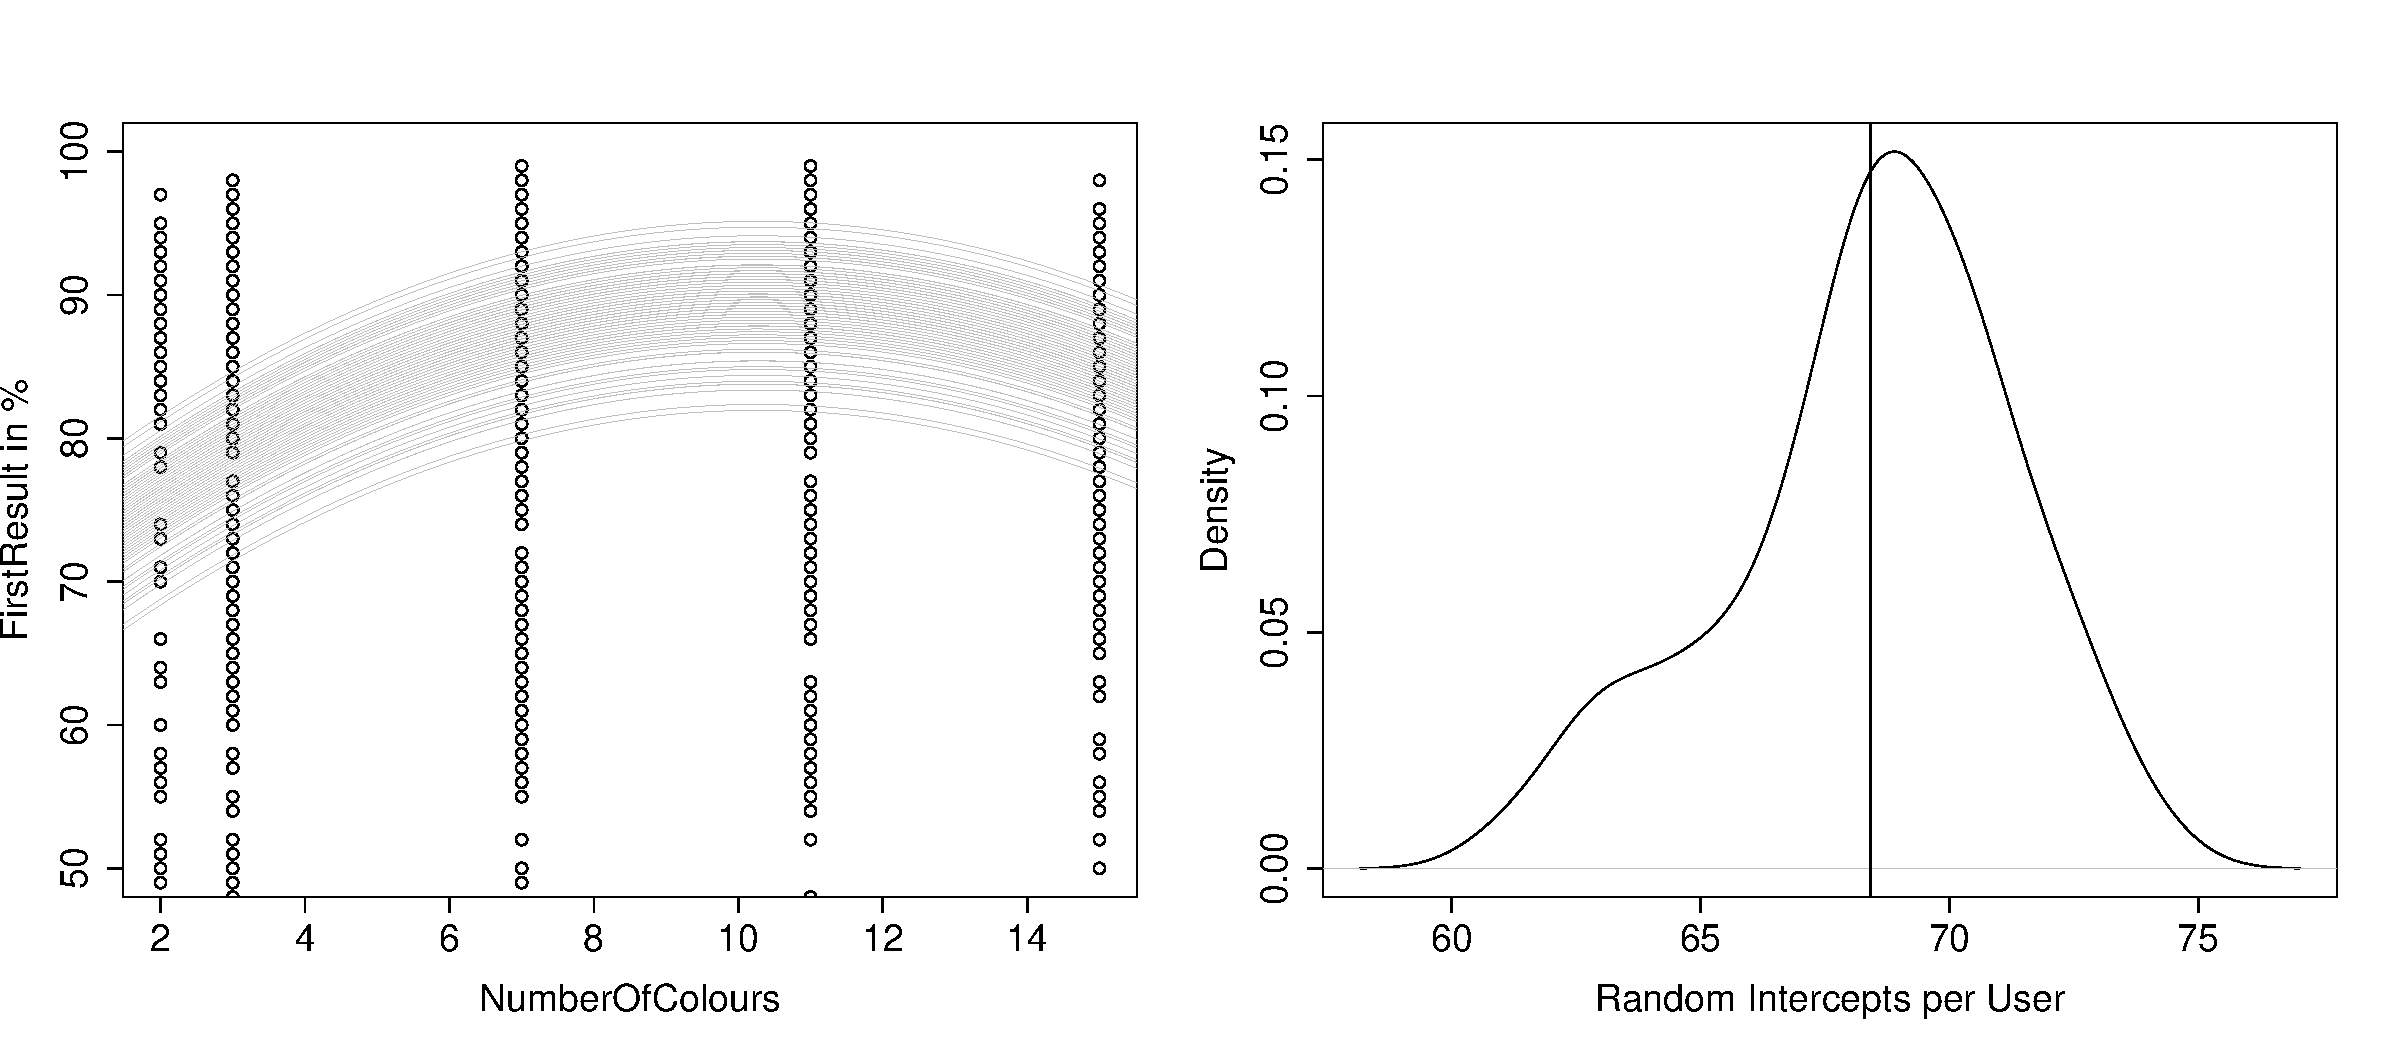
\includegraphics[width = 1\textwidth]{PlotIntercept.pdf}
%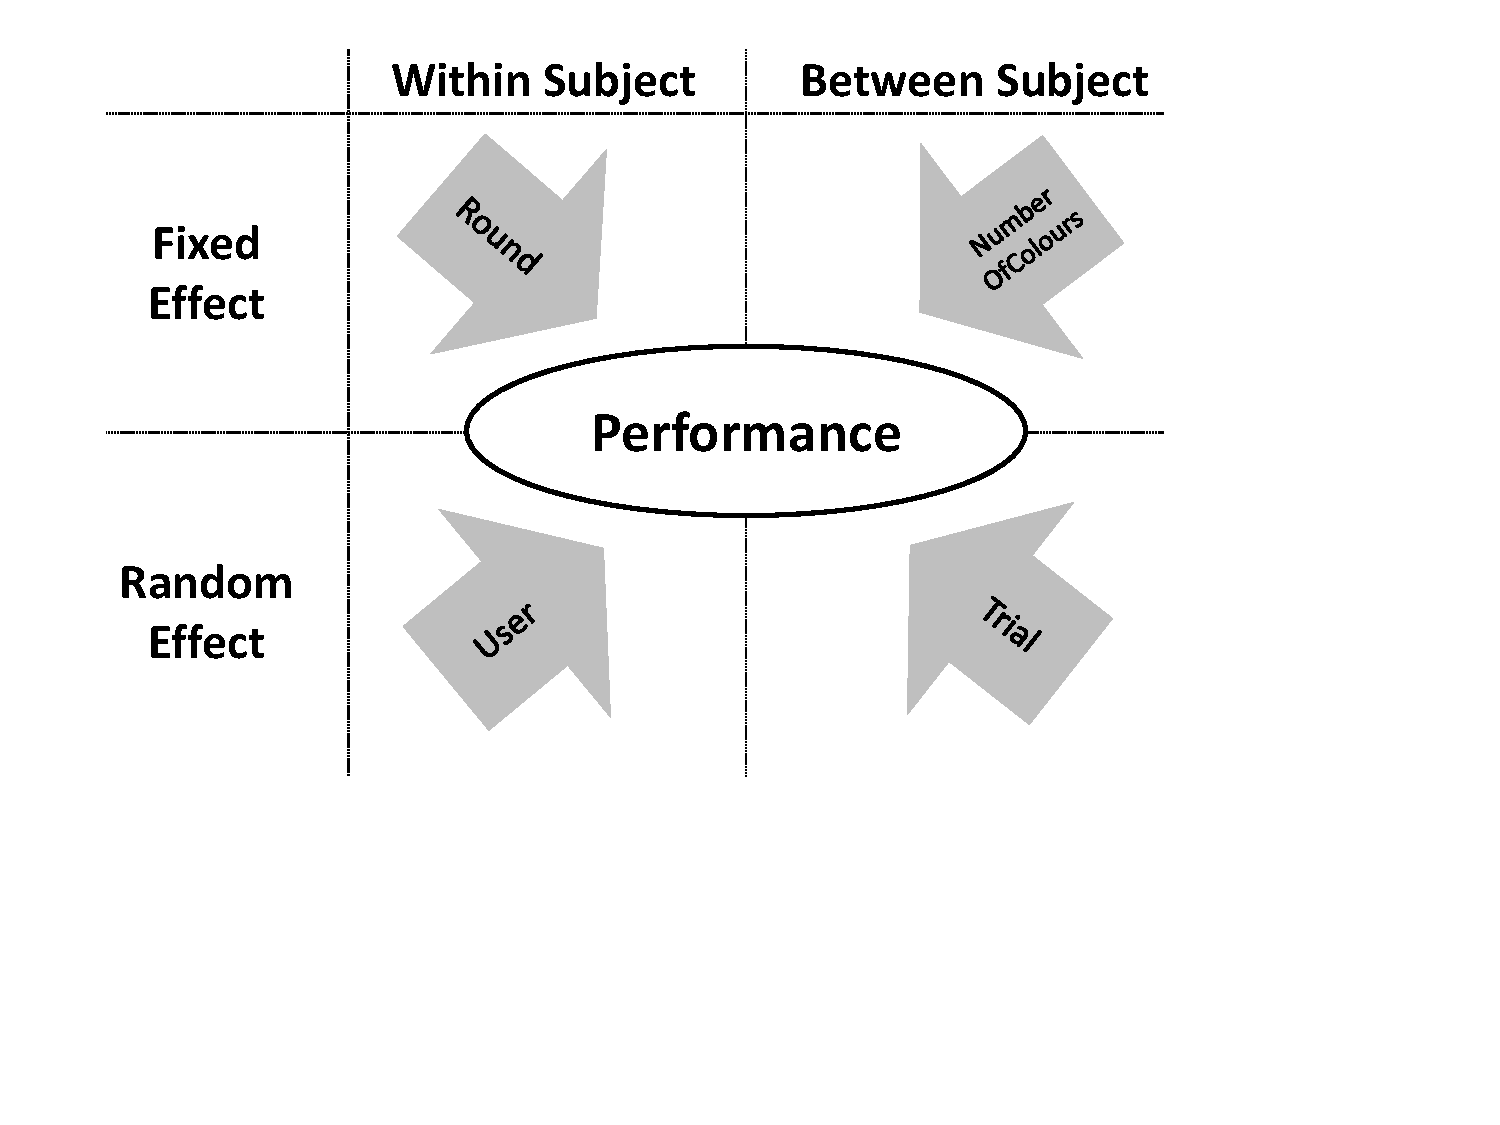
\includegraphics[height = 0.4\textwidth]{UserInfluence.pdf}
  \caption{User-individual Intercepts for the \textit{FirstResult}-parameters}
    \label{fig:Intercepts} 
\end{center}
\end{figure}
Second, we must determine whether the fixed effects are sufficient without a corresponding random effect. We assume that the performance is dependent on the individual characteristics of the participant. In other words, participants have a relatively equal sensitivity to \textit{NumberOfColours} and \textit{Round}, but perform on different levels due to the individual characteristics of each participant. Consequently, every participant has his or her own regression line, with a personalized intercept and an equal slope (Figure \ref{fig:Intercepts}). Due to the lack of influence by the \textit{Trial}, a nested classification of the random intercept is not necessary that would require a combination of \textit{Trial} and \textit{User} for the random intercept.\\
%To display these assumptions in a \ac{LMM}, we use a nested classification of the random intercept. A first random intercept covers the effects of the \textit{Trial} affiliation on the individual participant. Nested within the trial, a second random intercept is introduced to take into account the effects by the individual characteristics.\\
%The nested classification requires the participants to be bi-uniquely assigned to one trial and one usergroup \citep{Galecki2013}. By checking the \ac{AMT}-Worker ID, those participants who played both trials can be identified. Only 5 \ac{AMT}-Users were found, so the  bi-unique relation between user and trial can be assumed. Furthermore, we have excluded participants with the same IP address so that participants who played the game again and again were excluded and one participants consequently only played with one usergroup.\\
Third, correlations among repeated measurements must be taken into account. We assume that all rounds a user plays are equally correlated with each other and the total variation per round, $\sigma^{2} = \sigma^{2}_{\gamma} + \sigma^{2}_{\varepsilon}$, can be partitioned into the "shared" (user) component, $\sigma^{2}_{\gamma}$ and the "unshared" (round) component, $\sigma^{2}_{\varepsilon}$. \\
The \textit{Compound symmetry covariance matrix} is defined as:
\begin{equation}
\begin{split}
{\rm cov}(Y_{ij}, Y_{ik}) = \sigma^{2}_{\gamma} + \sigma^{2}_{\varepsilon} \cdot \mathcal{I}(k = j) \quad \quad \\
Y_{ij}:= Total\;Variance\;of\;User\;i\;in\;Round\;j
\end{split}
\end{equation}
Equation \ref{eq:LMM} shows the used single-level \ac{LMM} with random intercepts.

\fbox{%
\begin{minipage}{6 in}
\begin{equation}
\begin{split}
\label{eq:LMM}
DependentVariable_{i,j} = \quad\quad\quad\quad\quad\quad\quad\quad\quad\quad\quad\quad\quad\quad\quad\quad\quad\quad\quad\quad\quad\quad\quad\quad\quad\\
\boldsymbol{const} \quad\quad\quad\quad\quad\quad\quad\quad\quad\quad\quad\quad\quad\quad
\quad\quad\quad\quad\quad\quad\quad\quad\\
+ \boldsymbol{\beta_1} * NumberOfColours + \boldsymbol{\beta_2} * (NumberOfColours)^2\\
+ \boldsymbol{\beta_3} * log_{10} (Round) + \boldsymbol{r_{i}}+\epsilon_{i,j}\quad\quad\quad\quad\quad\quad\quad\quad
\end{split}
\end{equation}
    \begin{tabular}{ll}
    \textbf{Indexes} & $\;i := Participant,\;j := Round$  \\
    \textbf{Fixed effect 1} &  $\boldsymbol{\beta_1}$ * NumberOfColours + $\boldsymbol{\beta_2}$ * $(NumberOfColours)^2$\\
    \textbf{Fixed effect 2} &  $\boldsymbol{\beta_3} * log_{10}(Round)$\\
    \textbf{Random effect} &  $\boldsymbol{r_i}:=$ Random intercept per User i\\
    \textbf{Error} &  $\epsilon_{i,j}$\\
    \end{tabular}%
\end{minipage}}

\subsection{Implementation in R}

For the implementation of the \ac{LMM}s we use the \textbf{nlme}-package of the software programming language \textbf{R}\footnote{Refer to \cite{R2012}.} . The package is especially designed for \ac{LMM}s  \citep{Pinheiro2013} and fits a linear mixed-effects model in the formulation described by \cite{Laird1982}.\\
The model described in \ref{eq:LMM} is implemented using the following code:
\begin{verbatim}
> LMM <- lme(DV ~ 1 + NumberOfColours + NumberOfColours2 + RoundL, 
+               random=~1 | User, 
+               correlation=corCompSymm(form = ~ RoundL| User))
\end{verbatim}

\subsection{Results for the \ac{LMM}}

According to the conclusions for the \acl{NP}' results, only the filtered data is considered for the parameter estimations.\\
The results for the fixed effects of the \ac{LMM} can be interpreted in the same way as an ANOVA regression. Nevertheless, we must take into account that the intercept represents the mean over all subjects and each individual subject has its own individual intercept \citep{Seltman2012}. The population made up by all individual intercepts approximately follows a normal distribution, with the computed overall estimate as the mean and the variance of the random intercepts (Figure \ref{fig:Intercepts}).

\paragraph{Filter 1: Users with \textit{BestResult} $\geq$ 80\% for each round}
\textbf{\textit{NumberOfColours} }\\
The \ac{LMM} returns significant results for the \textit{FirstResult}, the \textit{DecisionTime} and the \textit{DecisionNumber}.  Moreover, they all have significant parameter estimations for all parameters. So the hypothesis that there is an \textbf{$\cap$}-relation between the performance of a participant and the \textit{NumberOfColours} is only supported for the \textit{FirstResult}. In addition, the results for \textit{DecisionTime} and \textit{DecisionNumber} show a polynomial relation with \textit{NumberOfColours}, as expected by the hypothesis. The \textit{DecisionTime} reaches its maximum and the \textit{DecisionNumber} its minimum for a medium level of information granularity. No significant results are signalized for the \textit{First-}, \textit{Best-}, and \textit{FinalTime}.

\afterpage{
\begin{landscape}
\begin{table}
\begin{center}
\begin{tabular}{l D{.}{.}{5.5} @{}D{.}{.}{5.5} @{}D{.}{.}{5.5} @{}D{.}{.}{5.5} @{}D{.}{.}{5.5} @{}D{.}{.}{5.5} @{}D{.}{.}{4.5}@{}D{.}{.}{4.5} @{}}
\toprule
                 & \multicolumn{1}{c}{First} & \multicolumn{1}{c}{Best} & \multicolumn{1}{c}{Final}  
                 & \multicolumn{1}{c}{First} & \multicolumn{1}{c}{Best} & \multicolumn{1}{c}{Final}
                 & \multicolumn{1}{c}{Decision} & \multicolumn{1}{c}{Decision}\\
                 & \multicolumn{1}{c}{Result} & \multicolumn{1}{c}{Result} & \multicolumn{1}{c}{Result} 
                 & \multicolumn{1}{c}{Time} & \multicolumn{1}{c}{Time}& \multicolumn{1}{c}{Time}
                 &\multicolumn{1}{c}{Number}& \multicolumn{1}{c}{Time} \\
\midrule
(Intercept)      & 85.46^{***}  & 89.82^{***}   & 89.40^{***}   & 44.09^{***}  & 53.50^{***}  & 63.38^{***}  & 2.26^{***}   & 28.91^{***} \\
                 & (1.29)       & (0.92)        & (0.97)        & (4.30)       & (4.44)       & (5.23)       & (0.18)        & (2.14)      \\
NumberOfColours  & 0.82^{*}     & 0.41          & 0.43          & 1.83         & 0.84         & 0.31         & 0.13^{**}     & -1.29^{*}   \\
                 & (0.36)       & (0.26)        & (0.27)        & (1.22)       & (1.23)       & (1.49)       & (0.05)        & (0.61)      \\
NumberOfColours2 & -0.05^{**}   & -0.03^{\cdot} & -0.03^{\cdot} & -0.10        & -0.02        & 0.03         & -0.01^{\cdot} & 0.07^{*}    \\
                 & (0.02)       & (0.01)        & (0.02)        & (0.07)       & (0.07)       & (0.09)       & (0.00)       & (0.03)      \\
RoundL           & 2.24^{\cdot} & 2.84^{***}    & 2.99^{***}    & -17.39^{***} & -16.16^{***} & -14.54^{***} & -1.21^{***}   & 4.86^{***}  \\
                 & (1.29)       & (0.76)        & (0.81)        & (3.37)       & (3.27)       & (3.25)       & (0.11)        & (1.40)      \\
\midrule
%Log Likelihood   & -1711.65     & -1470.47      & -1502.79      & -2252.97     & -2245.24     & -2274.95     & -527.98       \\
%$\sigma$: Intercept Trial &    <0.01    &    <0.01     &   <0.01      &  <0.01     &       <0.01 & <0.01 &  <0.01 \\
$\sigma$: Intercept User in Trial &   3.52     &     2.84    &      2.99 &13.62&  12.81     &    17.58   &   0.59  & 7.11 \\
$\sigma$: Residual         &     5.50   &    3.19   &    3.40    &       14.09&   14.72    &    13.45   & 0.47& 5.82\\
\bottomrule
\vspace{-3mm}\\
\multicolumn{9}{l}{\textsuperscript{***}$p<0.001$, 
  \textsuperscript{**}$p<0.01$, 
  \textsuperscript{*}$p<0.05$, 
  \textsuperscript{$\cdot$}$p<0.1$}
\end{tabular}
\caption{LMM-Results for Filter 1}
\label{table:coefficients}
\end{center}
\end{table}
\end{landscape}} 
\begin{figure}[H] % Filter1PlotColoursFirstResult	
\begin{center}
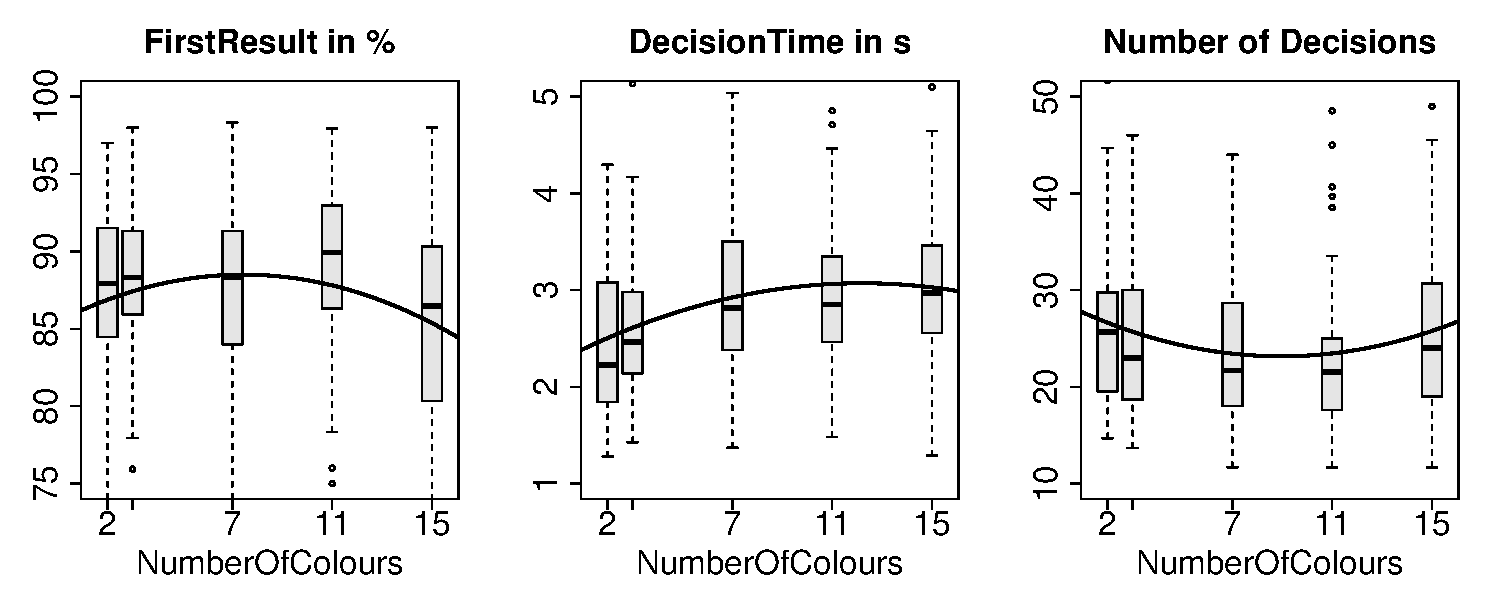
\includegraphics[width = 1\textwidth]{Filter2PlotInformationGranularity.pdf}    
  \caption[Results for Filter 1: Information Granularity]{Results for Filter 1: Information Granularity\footnotemark}
    \label{fig:Results for Filter 1: Information Granularity} 
\end{center}
\end{figure}
\footnotetext{The values for the dependent variables are adjusted so they exclude the predicted effect by \textit{Round}.}

\textbf{\textit{Round} }\\
The learning effect, hence the influence of the \textit{Round}, is significant for all variables. So we can conclude that there is a learning effect when playing several rounds in the experiment, and the slope of this learning effect diminishes with the number of rounds played, as indicated by the logarithmic relation. Surprisingly, the number of decisions increases with the number of rounds, as supposed to the expected decline. \\
Since the time it takes participants to reach the \textit{FinalResult} is represented by the product of \textit{DecisionNumber} and \textit{DecisionTime}, two opposing trends can be identified when describing the round effect on the \textit{FinalTime}. Whereas the number of decisions increases, the time to take a decision decreases. The \ac{LMM} returns a negative parameter for \textit{FinalTime},  indicating that the decrease in the decision times outbalances the increase in the number of decisions.  
\begin{figure}[H] % Filter1PlotColoursFirstResult	
\begin{center}
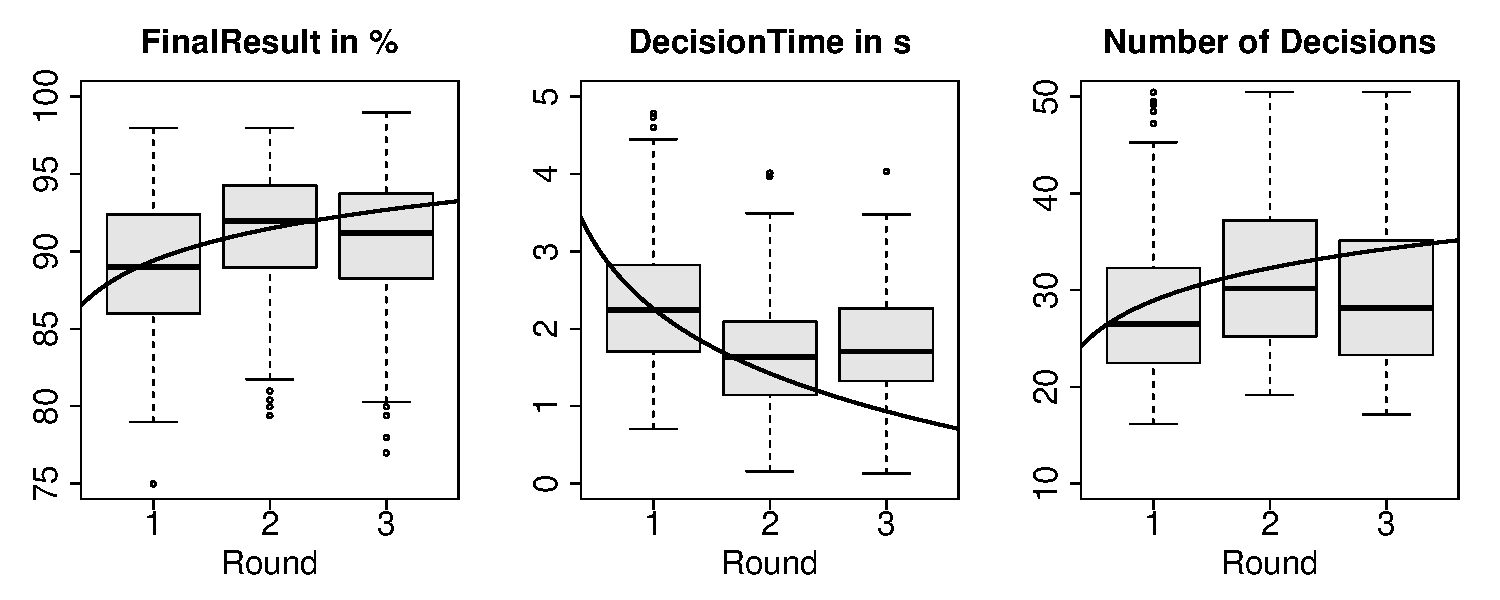
\includegraphics[width = 1\textwidth]{Filter2PlotLearningEffect.pdf}  
  \caption[Results for Filter 1: Learning effect]{Results for Filter 1: Learning effect\footnotemark}
    \label{fig:Results for Filter 1: Learning effect} 
\end{center}
\end{figure}
\footnotetext{The values for the dependent variables are adjusted so they exclude the predicted effect by \textit{NumberOfColours}.}
\textbf{\textit{User} }\\
The standard deviations of the \textit{User} random intercepts are high, and underline the influential magnitude of the individual performance characteristics of the participants. In particular, the \textit{DecisionNumber} and \textit{DecisionTime} seem to be most affected by the individual, since the relative standard deviation is the highest for all variables. 

%
%%\begin{landscape}
%\begin{table}
%\begin{center}
%\begin{tabular}{l D{.}{.}{5.5} @{}D{.}{.}{5.5} @{}D{.}{.}{5.5} @{}D{.}{.}{4.5} @{}D{.}{.}{5.5} @{}}
%\toprule
%                 & \multicolumn{1}{c}{First} & \multicolumn{1}{c}{Best} & \multicolumn{1}{c}{Final} & \multicolumn{1}{c}{Decision} &\multicolumn{1}{c}{Decision}\\
%                 & \multicolumn{1}{c}{Result} & \multicolumn{1}{c}{Result} & \multicolumn{1}{c}{Result} & \multicolumn{1}{c}{Time} &\multicolumn{1}{c}{Number}\\
%\midrule
%(Intercept)      & 85.46^{***}  & 89.82^{***}   & 89.40^{***}   & 2.26^{***}    & 28.91^{***} \\
%                 & (1.29)       & (0.92)        & (0.97)        & (0.18)        & (2.14)      \\
%NumberOfColours  & 0.82^{*}     & 0.41          & 0.43          & 0.13^{**}     & -1.29^{*}   \\
%                 & (0.36)       & (0.26)        & (0.27)        & (0.05)        & (0.61)      \\
%NumberOfColours2 & -0.05^{**}   & -0.03^{\cdot} & -0.03^{\cdot} & -0.01^{\cdot} & 0.07^{*}    \\
%                 & (0.02)       & (0.01)        & (0.02)        & (0.00)        & (0.03)      \\
%RoundL           & 2.24^{\cdot} & 2.84^{***}    & 2.99^{***}    & -1.21^{***}   & 4.86^{***}  \\
%                 & (1.29)       & (0.76)        & (0.81)        & (0.11)        & (1.40)      \\
%\midrule
%%AIC              & 3439.31      & 2956.94       & 3021.57       & 1071.96       & 3677.81     \\
%%BIC              & 3473.31      & 2990.94       & 3055.57       & 1105.96       & 3711.81     \\
%%Log Likelihood   & -1711.65     & -1470.47      & -1502.79      & -527.98       & -1830.91    \\
%%$\sigma$: Intercept Trial &    <0.01    &    <0.01     &   <0.01      &  <0.01     &       <0.01\\
%$\sigma$: Intercept User &   3.52     &     2.84    &      2.99 &   0.59  & 7.11 \\
%$\sigma$: Residual         &     5.50   &    3.19   &    3.40    &       0.47 & 5.82\\
%\bottomrule
%\vspace{-3mm}\\
%\multicolumn{6}{l}{\textsuperscript{***}$p<0.001$, 
%  \textsuperscript{**}$p<0.01$, 
%  \textsuperscript{*}$p<0.05$, 
%  \textsuperscript{$\cdot$}$p<0.1$}
%\end{tabular}
%\caption{LMM-Results for Filter 1}
%\label{table:coefficients}
%\end{center}
%\end{table}
%%\end{landscape}

\paragraph{Filter 2: Filter 1 + \textit{NumberOfColours} $\geq$ 7}
\textbf{\textit{NumberOfColours} }\\
When only including the treatment groups that were assigned to 7, 11 and 15 colours, the parameter estimations become significant for \textit{FirstResult}, \textit{BestResult} and \textit{FinalResult}. The \textbf{$\cap$}-relation with \textit{NumberOfColours} is consequently confirmed when looking at this range of \textit{NumberOfColours}. These findings, however, do not support our hypothesis that the performance will be best on a medium information granularity, since a peak can be found for the 11-colours treatment. In addition, none of the previous findings for \textit{DecisionNumber} and \textit{DecisionTime} are confirmed in Filter 2.\\
\textbf{\textit{Round} }\\
 A learning effect can also be detected for this data set, with an exception of \textit{FirstResult} - the \ac{LMM} does not return significant results for its parameters. \\
\textbf{\textit{User} }\\
The standard deviation for the \textit{User} random intercepts again show high values yet again, so the impact of excluding the variance caused by individual characteristics is underlined.\\

\begin{figure}[H] % Filter1PlotColoursFirstResult	
\begin{center}
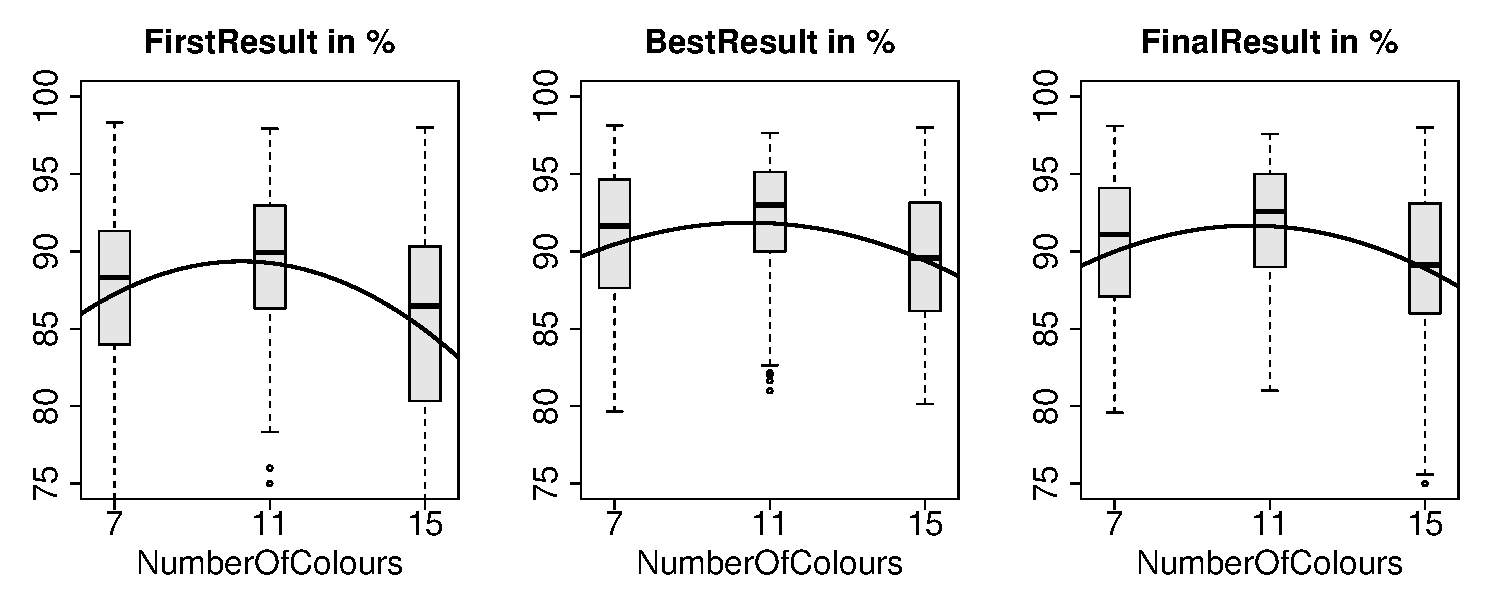
\includegraphics[width = 1\textwidth]{Filter3PlotInformationGranularity.pdf}    
  \caption[Results for Filter 2: Information Granularity]{Results for Filter 2: Information Granularity\footnotemark}
    \label{fig:Results for Filter 3: Information Granularity} 
\end{center}
\end{figure}
\footnotetext{The values for the dependent variables are adjusted so they exclude the predicted effect by \textit{Round}.}

%\afterpage{
%\begin{landscape}
%\begin{table}
%\begin{center}
%\begin{tabular}{l D{.}{.}{5.5} @{}D{.}{.}{4.5} @{}D{.}{.}{4.5} @{}D{.}{.}{5.5} @{}D{.}{.}{5.5} @{}D{.}{.}{5.5} @{}D{.}{.}{4.5} @{}}
%\toprule
%                 & \multicolumn{1}{c}{FirstResult} & \multicolumn{1}{c}{BestResult} & \multicolumn{1}{c}{FinalResult} & \multicolumn{1}{c}{FirstTime} & \multicolumn{1}{c}{BestTime} & \multicolumn{1}{c}{FinalTime} & \multicolumn{1}{c}{DecisionTime} \\
%\midrule
%(Intercept)      & 68.41^{***} & 78.95^{***} & 76.55^{***} & 54.92^{*}    & 84.20^{***} & 102.08^{***} & 3.34^{***}  \\
%                 & (6.87)      & (5.13)      & (5.34)      & (22.90)      & (22.49)     & (26.06)      & (0.94)      \\
%NumberOfColours  & 4.08^{**}   & 2.47^{*}    & 2.88^{**}   & -0.25        & -5.34       & -7.31        & -0.07       \\
%                 & (1.36)      & (1.01)      & (1.05)      & (4.52)       & (4.44)      & (5.15)       & (0.19)      \\
%NumberOfColours2 & -0.20^{**}  & -0.12^{*}   & -0.14^{**}  & 0.00         & 0.26        & 0.36         & 0.00        \\
%                 & (0.06)      & (0.05)      & (0.05)      & (0.21)       & (0.20)      & (0.23)       & (0.01)      \\
%RoundL           & 2.26        & 3.73^{***}  & 3.64^{***}  & -18.79^{***} & -12.15^{**} & -11.47^{**}  & -1.31^{***} \\
%                 & (1.43)      & (0.96)      & (1.03)      & (4.32)       & (4.25)      & (4.03)       & (0.15)      \\
%\midrule
%Log Likelihood   & -1059.20    & -940.58     & -960.30     & -1429.44     & -1423.93    & -1427.96     & -351.77     \\
%$\sigma$: Intercept Trial &    <0.01    &    <0.01     &   <0.01      &  <0.01     &       <0.01 & <0.01 &  <0.01 \\
%$\sigma$: Intercept User in Trial &    4.16    &   3.22      &     3.31    &      14.35 &     14.09  & 16.87 & 0.61  \\
%$\sigma$: Residual         &    4.77    &     3.17    &    3.43    &    14.25   &   14.02    &     13.32  & 0.49\\
%\bottomrule
%\vspace{-3mm}\\
%\multicolumn{8}{l}{\textsuperscript{***}$p<0.001$, 
%  \textsuperscript{**}$p<0.01$, 
%  \textsuperscript{*}$p<0.05$, 
%  \textsuperscript{$\cdot$}$p<0.1$}
%\end{tabular}
%\caption{LMM-Results for Filter 2}
%\label{table:Filter2Results}
%\end{center}
%\end{table}
%\end{landscape}}


\begin{table}
\begin{center}
\begin{tabular}{l D{.}{.}{5.5} @{}D{.}{.}{4.5} @{}D{.}{.}{4.5} @{}D{.}{.}{5.5} @{}D{.}{.}{5.5} @{}D{.}{.}{5.5} @{}D{.}{.}{4.5} @{}}
\toprule
                 & \multicolumn{1}{c}{First} & \multicolumn{1}{c}{Best} & \multicolumn{1}{c}{Final} & \multicolumn{1}{c}{Decision} &\multicolumn{1}{c}{Decision}\\
                 & \multicolumn{1}{c}{Result} & \multicolumn{1}{c}{Result} & \multicolumn{1}{c}{Result} & \multicolumn{1}{c}{Time} &\multicolumn{1}{c}{Number}\\
\midrule
(Intercept)      & 68.41^{***} & 78.95^{***} & 76.55^{***} & 3.34^{***}  & 36.34^{***} \\
                 & (6.87)      & (5.13)      & (5.34)      & (0.94)      & (10.85)     \\
NumberOfColours  & 4.08^{**}   & 2.47^{*}    & 2.88^{**}   & -0.07       & -2.78       \\
                 & (1.36)      & (1.01)      & (1.05)      & (0.19)      & (2.14)      \\
NumberOfColours2 & -0.20^{**}  & -0.12^{*}   & -0.14^{**}  & 0.00        & 0.14        \\
                 & (0.06)      & (0.05)      & (0.05)      & (0.01)      & (0.10)      \\
RoundL           & 2.26        & 3.73^{***}  & 3.64^{***}  & -1.31^{***} & 6.26^{***}  \\
                 & (1.43)      & (0.96)      & (1.03)      & (0.15)      & (1.63)      \\
\midrule
AIC              & 2134.39     & 1897.16     & 1936.59     & 719.54      & 2288.81     \\
BIC              & 2164.69     & 1927.46     & 1966.89     & 749.84      & 2319.11     \\
Log Likelihood   & -1059.20    & -940.58     & -960.30     & -351.77     & -1136.41    \\
%$\sigma$: Intercept Trial &    <0.01    &    <0.01     &   <0.01      &  <0.01     &       <0.01 \\
$\sigma$: Intercept User&    4.16    &   3.22      &     3.31    & 0.61  & 7.10\\
$\sigma$: Residual         &    4.77    &     3.17    &    3.43    & 0.49 & 5.33\\
\bottomrule
\vspace{-3mm}\\
\multicolumn{6}{l}{\textsuperscript{***}$p<0.001$, 
  \textsuperscript{**}$p<0.01$, 
  \textsuperscript{*}$p<0.05$, 
  \textsuperscript{$\cdot$}$p<0.1$}
\end{tabular}
\caption{LMM-Results for Filter 2}
\label{table:Filter2Results}
\end{center}
\end{table}



%%% ===============================
%\section{Hypotheses Test}
%\label{ch:Evaluation:sec:HypothesesTest}
%%% ===============================
%
%For all hypotheses, we define the null hypothesis as a point hypothesis, which states that the means for all treatments are the same. The alternative hypotheses can be expressed by saying: "at least one of the treatment means differ from all the others".
%\begin{equation}
%\begin{split}
%NumberOfColours: \mu_1=\dots=\mu_4  \\
%Round: \mu_1=\dots=\mu_3 \\
%\mu_i = mean \quad
%\end{split}
%\end{equation}
%
%that all means for the outcome variables the variable \textit{number of colours} has no significant influence on the outcome variables FirstResult, BestResult, FinalResult and DecisionTime.
%
%Linear transformation Number of COlours 4x+3
%The extracted data is used to test the hypothesis introduced in Section \ref{ch:Literature Review:sec:Hypotheses}.
%
%\begin{table}[htbp] % Usergroup and Hypotheses
%  \centering
%  \caption{Usergroups and Nullhypotheses}
%  \label{tab:NullHypotheses}
%    \begin{tabular}{cc|rrr}
%    \toprule
%    \textbf{Usergroup} & \textbf{\# Colours} & \multicolumn{3}{c}{\textbf{Null Hypotheses}} \\
%    \midrule
%    \textbf{1} & 3     & \textbf{} & \multicolumn{1}{l}{H1a-c: } & \multicolumn{1}{l}{   $\mu_1=\dots=\mu_4$ } \\
%    \textbf{2} & 7     &       & \multicolumn{1}{l}{H2} & \multicolumn{1}{l}{Usergroup 2+3 > 1+4} \\
%    \textbf{3} & 11    &       & \multicolumn{1}{l}{H3a-c: } & \multicolumn{1}{l}{Round 1 < 2 < 3} \\
%    \textbf{4} & 15    & \textbf{} & \multicolumn{1}{l}{H4} & \multicolumn{1}{l}{Round 1 < 2 < 3} \\
%    \bottomrule
%    \end{tabular}%
%\end{table}%
%


%% conclusion.tex
%%

%% ==================
\chapter{Conclusion}
\label{ch:Conclusion}
%% ==================

In this section, the conclusions from the evaluation section are drawn and potential limitations of the result are discussed. Furthermore, lessons learned from the experiment are described and potential fields of further research are examined.

\paragraph{\acf{AMT} and the quality of data}
As indicated by the findings of the \acl{NP}, the data generated on \ac{AMT} includes a lot of noise. Many participants failed to get a result higher than 80\%, a level which can be considered as fairly easy to achieve. Even increasing the leverage of the bonus and the total possible payout did not show to have an influence on the participants. So we must conclude, that offering the experiment as a \ac{HIT} on \ac{AMT} will return a lot of data that is not usable for the analysis of statistical implications. The advantages of a computer-lab experiment therefore lay in the quality of the data since the intrinsic motivation of participants is likely to be higher.

\paragraph{The level of information granularity affects the \textit{FirstResult}, \textit{DecisionTime} and \textit{DecisionNumber}.}
When focusing the statistical analysis on the participants who made an effort to succeed in the game, the statistical results indicate that an information overload has materialized. In fact, the highest performance is achieved on a medium level of information granularity for the first result that the participants offer. These findings are in particular interesting because we argue that users of smart meters have an interest in achieving a satisfying result in a minimum time, since they divide their time between many things.\\
The findings for the \textit{DecisionTime} indicate that users facing a medium level of information granularity take the most time to make a decision. These results indicate an information overload and can be explained by Jacoby's thesis that one must differentiate between the questions "Can consumers be overloaded?" and "Will consumers be overloaded?". 
Individuals facing an information overload might not directly experience this information overload while making their choice, because they only concentrate on a part of the given information prior to their decision. In other words, individuals confronted with an information overload are selective in their information selection and stop \textit{"far short of overloading themselves"} \citep{Jacoby1984}.\\
A participant on a medium level of information granularity is just at the border of an information overload - the individual can still cope with the amount of information. Since the given information provides more detail than a lower level of information granularity, we can define three consequences:
\begin{itemize}
\item The choice is supported by a better understanding of the underlying parameter (Benefit) and therefore the choice accuracy increases $\Rightarrow$ \textit{FirstResult}.
\item Due to the amount of information to process, it takes the individual more time to make the decision $\Rightarrow$ \textit{DecisionTime}.
\item Since the choice accuracy and the decision time increase, the individual makes fewer decisions $\Rightarrow$ \textit{DecisionNumber}.
\end{itemize}
When being provided with more information, the information processing gets selective, so the actual amount of information that is considered for the choice might decrease. Therefore, both the choice accuracy and the decision time decrease, the number of decisions increases.\\
In addition, when excluding the lower levels of information granularity, the results of the statistical model indicate that the best performance can be achieved on a medium-to-high level of information granularity. These findings are not described in our original hypothesis, but have implications for the further development of the experiment. 
\textbf{TO DOO!!!}

\paragraph{Learning Effect has a influence on the performance and the game time} 

Participants improve their performance with a growing number of played rounds, yet the magnitude of the learning effect diminishes over the number of rounds. So for the identified information overload in reaching the \textit{FirstResult}, we can conclude that individuals find strategies to cope with information overload when they get more experienced in this situation. A potential question to ask for future is how these findings are reflected in a setup that includes more rounds.

\paragraph{Individual characteristics affect the the performance}
Individual characteristics has proven to be influential on the participants. Even tough participants might show a similar sensitivity to the level of information granularity, their performances are affected by individual factors. Taking into account these effects when setting up a statistical model helps to exclude influences such as limited attention while playing the game or an individual talent for succeeding in these types of experiments. As a result, limitations of the \acl{AMT} and there negative consequences on statistical results can be tackled by the design of the statistical model.


%
%One reason for the lack of a detectable learning effect might be the trial round prior to the game. This opportunity enabled the participants to spend as much time as desired on exploring the experiment and on trying different strategies. As indicated by the timelog analysis in Section \ref{ch:Experiment:sec:DataacquisitionDescriptives}, the participants spent the majority of their time on the explanation part and used the chance to get familiar with the experiment. The trial round was necessary to ensure that participants were fully aware of the task and the design of the experiment. Yet, the learning curve already started here, participants could improve their performance without any time pressure and were used to the implemented information overload. The findings for the final performance from Round 1 and 2 might be an indication that the learning effect continued for the first 2 rounds. Having said that, one would expect the final performance for Round 3 to be at least the level of the performance in Round 2, yet usergroup 3 and 4 reduce their performance in Round 3.\\
%The lack of a learning effect is interesting since prior research with a similar experiment \citep{Schmidt2012} gave an indication that a learning effect is significant. In contrast to our setup, Schmidt's experiment included 13 runs, so 
%
%excluding those participants who were not able to perform better than 80\%
%
%
%As indicated by the findings of the \acl{NP}, the data generated on \ac{AMT} includes a lot of noise. Many participants failed to get a result higher than 80\%, a level which can be considered as fairly easy to achieve. Even increasing the leverage of the bonus and the total possible payout did not show to have an influence on the participants. So we must conclude, that offering the experiment as a \ac{HIT} on \ac{AMT} will return a lot of data that is not usable for the analysis of statistical implications. The advantages of a computer-lab experiment clearly lay in the quality of the data.
%
%
%
%
%\section{Information Granularity}
%
%The influence of the information granularity has not shown the expected magnitude since all the related hypotheses are rejected. Nevertheless, a comparison between a low information granularity and a high information granularity - usergroup 1 and 4 - returns significant results, indicating, that a low information granularity leads to better choice accuracy. 
%
%In order to back up these findings, further research might add more colours to the framework to prove the negative correlation between number of colours and performance. A small change for the number of colours between treatments did not emerge to be the right approach to get distinctive results for each treatment, so we would suggest to increase the number of colours with a larger step size, e.g. introducing 27 or more colours. This approach might be more successful in finding a significant relationship between information granularity and choice accuracy.\\
%Yet, the reason for the lack of significant results for a medium information granularity must be further discussed. When the number of colours is increased, two opposing trends in the complexity of the game can be identified. As the number of colours increases, the color frame gets more complex and the dimension of the attribute level \textit{benefit} increases. This development reinforces the information load, as indicated by \cite{Jacoby1974} and \cite{Malhotra1982}. In contrast to that, with a growing number of colours, the benefit range covered by one colour decreases, so the choices get more specific and accurate. Whereas participant 1 who faces a low number of colours can choose between colours that represent a wide range of benefit, participant 2 who is challenged with a high number of colours can choose among colours that represent a more specific benefit value. Consequently, the participant 2 is less dependent on the chance that he or she clicks a box with a high benefit within the benefit range, but can make a more conscious choice.\\
%These two opposing trends might be one reason why there is no clear development detectable for increasing number of colours. Reducing the complexity of the game to a controllable, one-dimensional approach would be a potential for future research. In the forefront of the experiment, several interfaces were open for discussion. The implemented approach was chosen because it guaranteed the comparability among usergroups, since the underlying knapsack problems are the same. If future research finds a way to combine comparability and one-dimensional complexity, the findings might get clearer for the influence from information granularity. One approach would be to assign one specific value per colour. This will result in different benefit ranges for each treatment and challenge the comparability of the problems. Yet, by using the delta-benchmark that was applied for the comparability between rounds, researchers can control the difficulty of the underlying problems and can consequently control comparability.
%
%\section{Learning Effect}
%
%

\section{Limitations of the experiment}
%As stated in Section \ref{ch:Evaluation:sec:DescriptiveStatistics:subsec:Distributionofusergroups}, the distribution of participants among usergroup was not uniformly. Since we saw a higher dropout-rate for usergroups with a higher number of colour, the representation of the population mean in each usergroup might be diluted. As participants drop out of usergroups 2, 3 and 4, the data is skewed towards participant in usergroup who face a lower information load. Our findings would be therefore suspect, if the performance of usergroup 1 was worse than the performance of all usergroups since the better performance of usergroup 2, 3 and 4 might be related to the dropout of participants who were unable to cope with the information overload.
In order to make the experiment as intuitive and straight-forward as possible, a considerable level of abstraction is necessary. This helps participants to better understand the given task, but also implies a simplification of the information environment the real-life smart-meter user is usually confronted with\footnote{Refer to \cite{Jacoby1984}}. The experiment has proven an
an information overload in the simplified game environment. So we can argue that these results lead to the conclusion that an information overload would occur under a more complex experiment setup, e.g. analysing the data provided by a smart-meter. 
In contrast to that, the undetectable information overload in the simplified experiment for the best performances of a participants does not result to the conclusion that there will not be an information overload in a more complex experiment environment.



\textbf{BonusSystem better incentive to play better, since the two bonus systems weren ot successsfull}
%
%
%The design of the experiment requires a
%Oversimplification of information overload experiments 433 \cite{Jacoby1984}
%
%Control group with 3, 7, 11, 15
%
%No Random treatment assignment!! ==> No representation of population mean
%\dots

%
%
%\begin{table}[p]%
%\centering
%\parbox{0.4\textwidth}{
%\begin{footnotesize}
%\begin{tabular}{l D{.}{.}{3.5} @{}}
%\toprule
%                 & \multicolumn{1}{c}{Parameters} \\
%\midrule
%(Intercept)      & -4.08^{\cdot} \\
%                 & (1.90)        \\
%NumberOfColours  & 1.84^{**}     \\
%                 & (0.59)        \\
%NumberOfColours2 & -0.10^{*}     \\
%                 & (0.03)        \\
%\midrule
%R$^2$            & 0.49          \\
%Adj. R$^2$       & 0.41          \\
%Num. obs.        & 15            \\
%\bottomrule
%\vspace{-3mm}\\
%\multicolumn{2}{l}{\textsuperscript{***}$p<0.001$, 
%  \textsuperscript{**}$p<0.01$, 
%  \textsuperscript{*}$p<0.05$, 
%  \textsuperscript{$\cdot$}$p<0.1$}
%\end{tabular}
%\end{footnotesize}
%\caption{Parameter estimations}
%\label{tab:table}
%}
%\qquad
%\begin{minipage}[c]{0.4\textwidth}%
%\centering
%    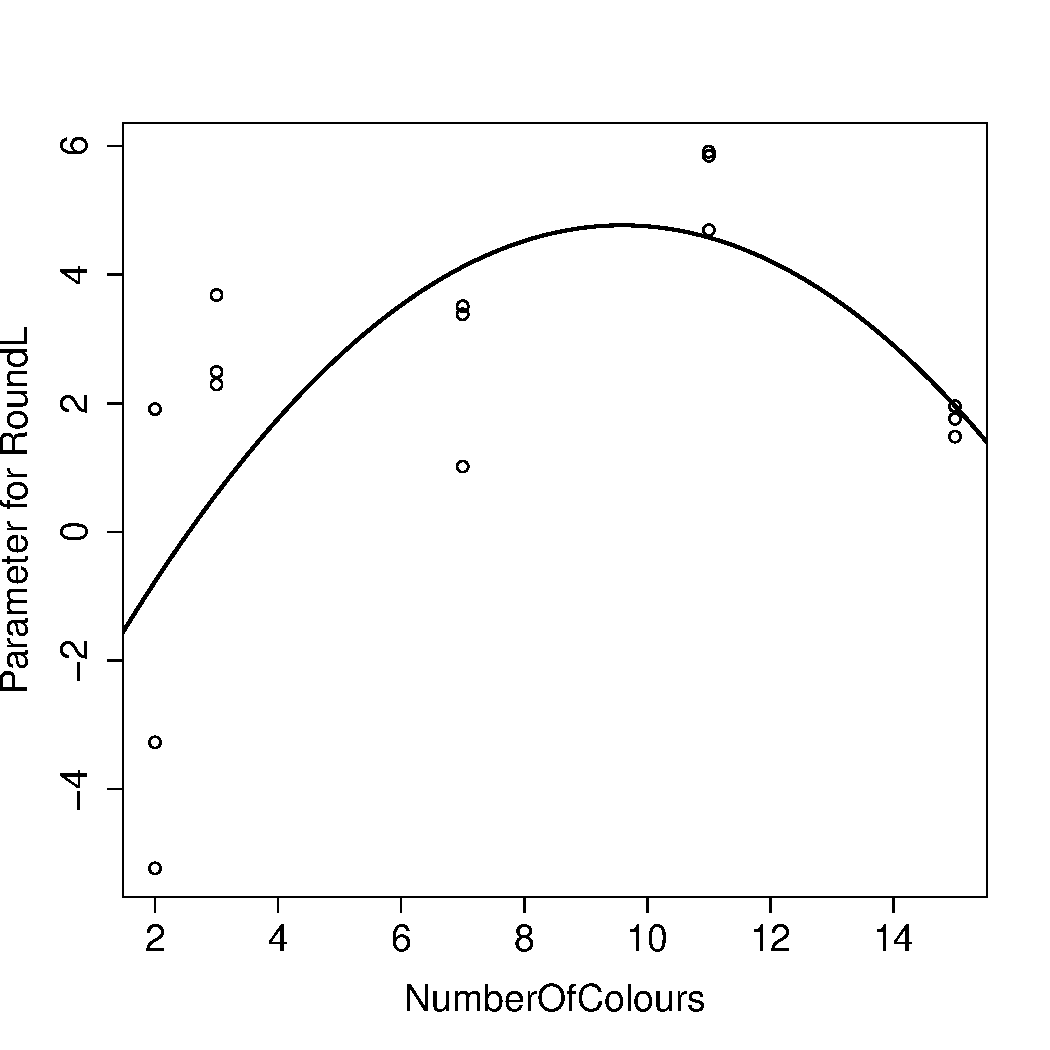
\includegraphics[width=1\textwidth]{PlotColoursLearningEffect.pdf}
%\caption{Plot Parameters over NumberOfColours}
%\label{fig:figure}
%\end{minipage}
%\end{table}
%% declaration.tex
%%

%% ==================
\iflanguage{english}
{\chapter{Declaration}}
{\chapter{Erklärung}}
\label{ch:Declaration}
%% ==================

Ich versichere hiermit wahrheitsgemäß, die Arbeit selbstständig verfasst und keine anderen als die angegebenen Quellen und Hilfsmittel benutzt, die wörtlich oder inhaltlich übernommenen Stellen als solche kenntlich gemacht und die Satzung des Karlsruher Instituts für Technologie (KIT) zur Sicherung guter wissenschaftlicher Praxis in der jeweils gültigen Fassung beachtet zu haben.

\vspace*{1cm}
\hspace*{4cm} Karlsruhe, den \submissiontime \hspace*{0.5cm}\hrulefill \\
\hspace*{10.5cm} \myname \\




%% ----------------
%% |   Appendix   |
%% ----------------
% IM Style: No additional blank page
%\cleardoublepage

%% appendix.tex
%%

%% ==============================
%\chapter{Appendix}
%\label{ch:Appendix}
%% ==============================

\appendix

\iflanguage{english}
{\addchap{Appendix}}	% english style
{\addchap{Anhang}}	% german style

\section{Algorithm}
		\label{Appendix-Algorithm}
		
\begin{algorithm}[h] % setup Rounds
\LinesNumbered
\SetNoFillComment
\setcounter{AlgoLine}{0}
 \SetAlgoLined
 \tcc{rounds:= 4 rounds; 4 usergroups}
  \KwIn{rounds, usergroups }
 \KwResult{4 Rounds per each usergroup }

 benchmarkCurrent = 0\;
 
\ForAll{rounds}{
\tcc{100 iterations}
 \For{i=0 to 100}{
 \tcc{100 Boxes}
 \For{j=0 to 100}{
 	width = uniform random in range of 20 and 80\;
 	

 	benefit = uniform random in range of 0 and 80\;
 	
 	create Box with width and benefit
 }\;

benchmark = (\ac{DPA} Solution / \ac{GA} Solution\ - 1) x 100\%;
 
 \If{benchmarkCurrent $\leq$ benchmark}{
 	benchmarkCurrent = benchmark
 	
 	  \tcc{itemsHardProblem:= save current boxes }
 
 	boxesHardProblem = boxes
 	}
 }

 \ForAll{ boxes in boxesHardProblem}{
 \ForAll{usergroups}{
 new Box (box.benefit, box.weight, current round)\;
 
 add colour according to benefit and number of colours\;
} 	
 } }
\caption{Setup of rounds}
\label{Setup of rounds}
\end{algorithm}

\newpage
\section{Interface for each usergroup}
		\label{Appendix-Implementation}
		
\setcounter{figure}{0}
\begin{figure}[htbp] % DistributionFinalResult
\begin{center} 
\begin{subfigure} 
\centering
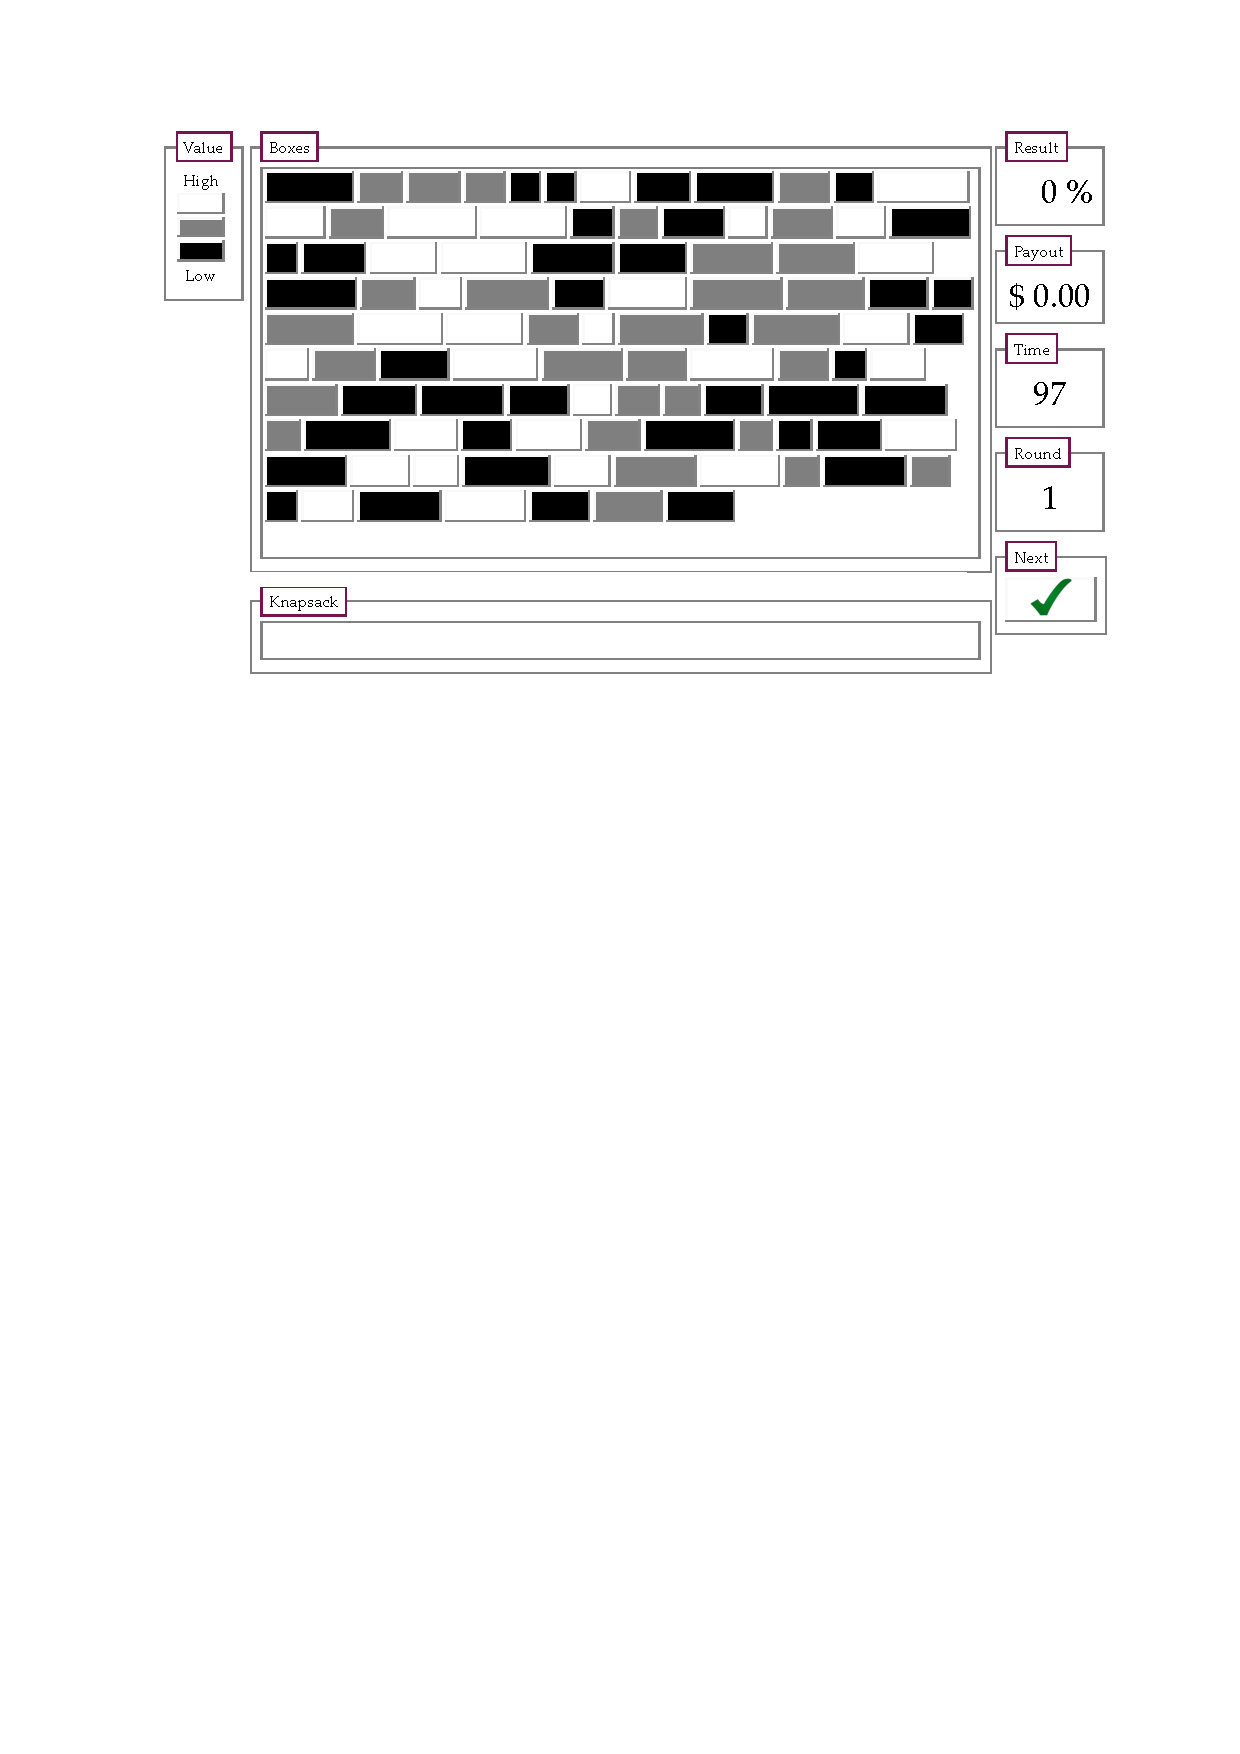
\includegraphics[height = 0.39\textwidth]{Interface1.pdf}
\end{subfigure} 
\begin{subfigure} 
\centering
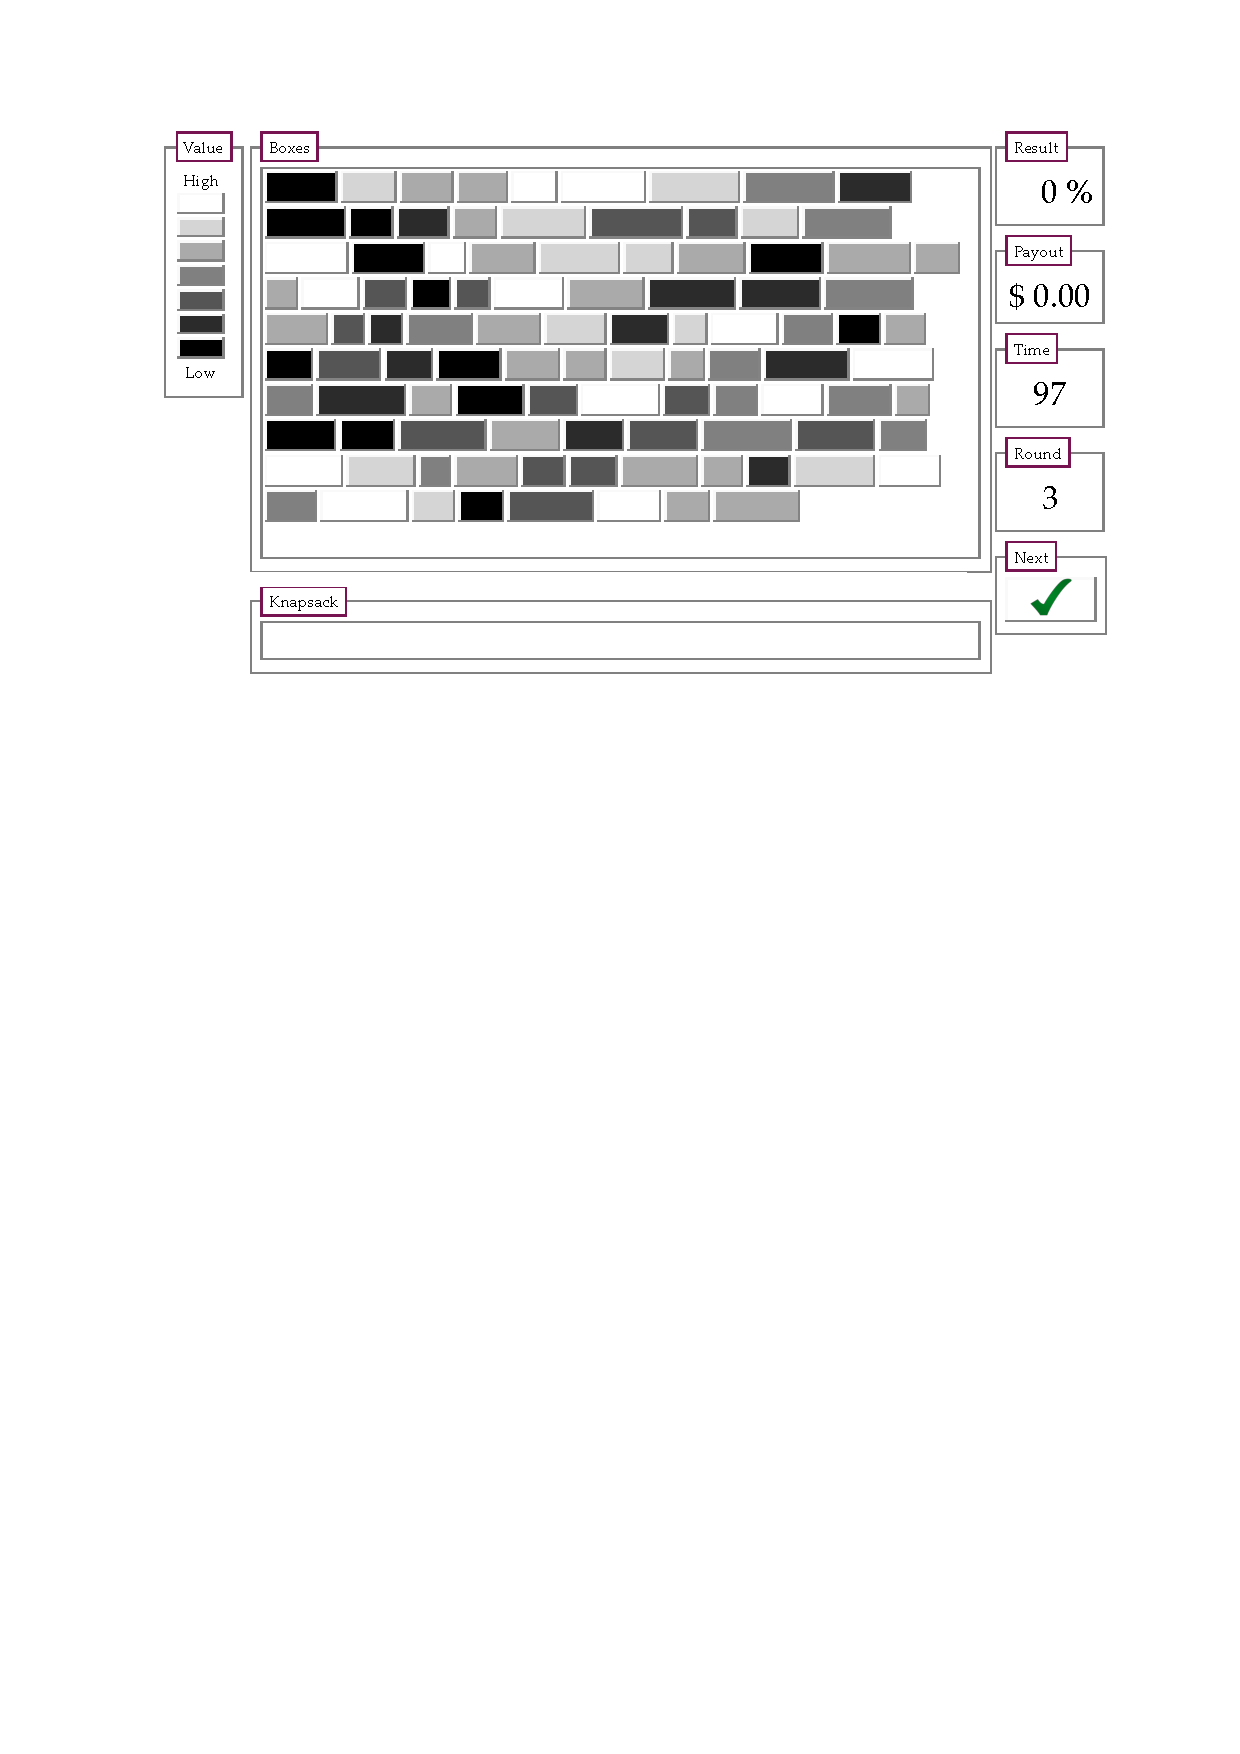
\includegraphics[height = 0.39\textwidth]{Interface2.pdf}
\end{subfigure}
\begin{subfigure} 
\centering
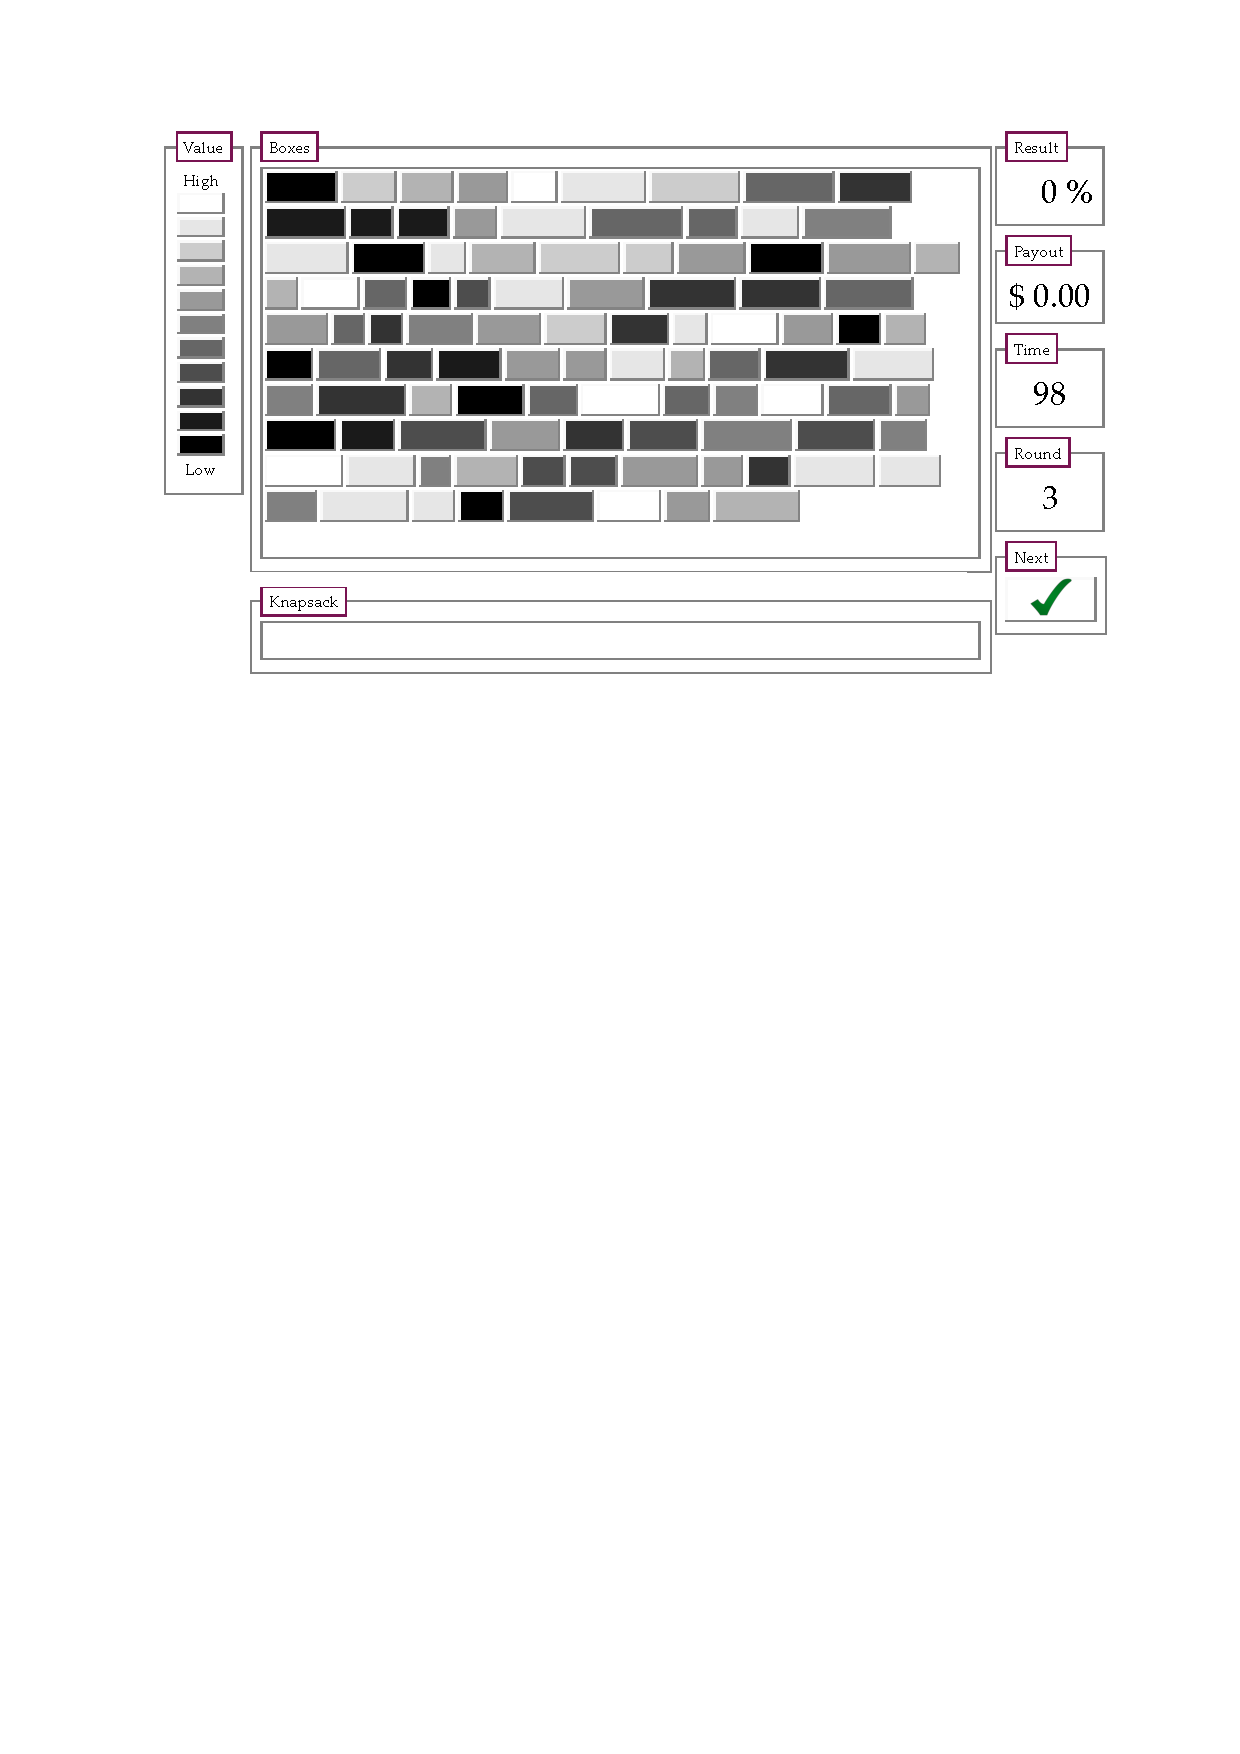
\includegraphics[height = 0.39\textwidth]{Interface3.pdf}
\end{subfigure}
  \caption{Interface for Usergroup 1, 2  and 3}
    \label{InterfaceOverview} 
\end{center}
\end{figure}

\newpage

\section{Formulas}
		\label{Appendix-Formulas}

%\begin{figure}[htbp]
%\begin{equation}
%\begin{split}
%x' = \dfrac{1}{4}x+\dfrac{1}{4},\;x = 3,7,11,15\quad \quad \quad\\ 
%x := number\;of\;colours,\;x' := new\;variable
%\end{split}
%\end{equation}
%\caption{Number of colours - Usergroup}
%\label{NumberUsergroup}
%\end{figure}
\begin{equation}
\begin{split}
Share\;of\;dropout = \dfrac{p_i(user|dropout)}{p_i(user)}, \quad \quad \\ 
i = 1,..4,\;user := number\;of\;users\;logged\;in
\end{split}
\end{equation}

\begin{equation}
\begin{split}
Share\;of\;minimum\;payout = \dfrac{p_i(user|payout=0)}{p_i(user)}, \\ 
i = 1,..4, user := number\;of\;users \quad \quad
\end{split}
\end{equation}

\begin{figure}[htbp]
\caption{Box - Cox - Transformation}
\label{BoxCoxTransformation}
\begin{equation}
y_i^{(\lambda)} = \begin{cases}
\dfrac{y_i^{\lambda}-1}{\lambda}, \quad if \lambda \neq 0, \\ 
log(y_i), \quad if \lambda = 0
\end{cases}, \quad y > 0 
\end{equation}

\end{figure}

\section{Descriptive statistics}
		\label{Appendix-Descriptive}
		
\begin{figure}[htbp] % DistributionFirstResult
\begin{center} 
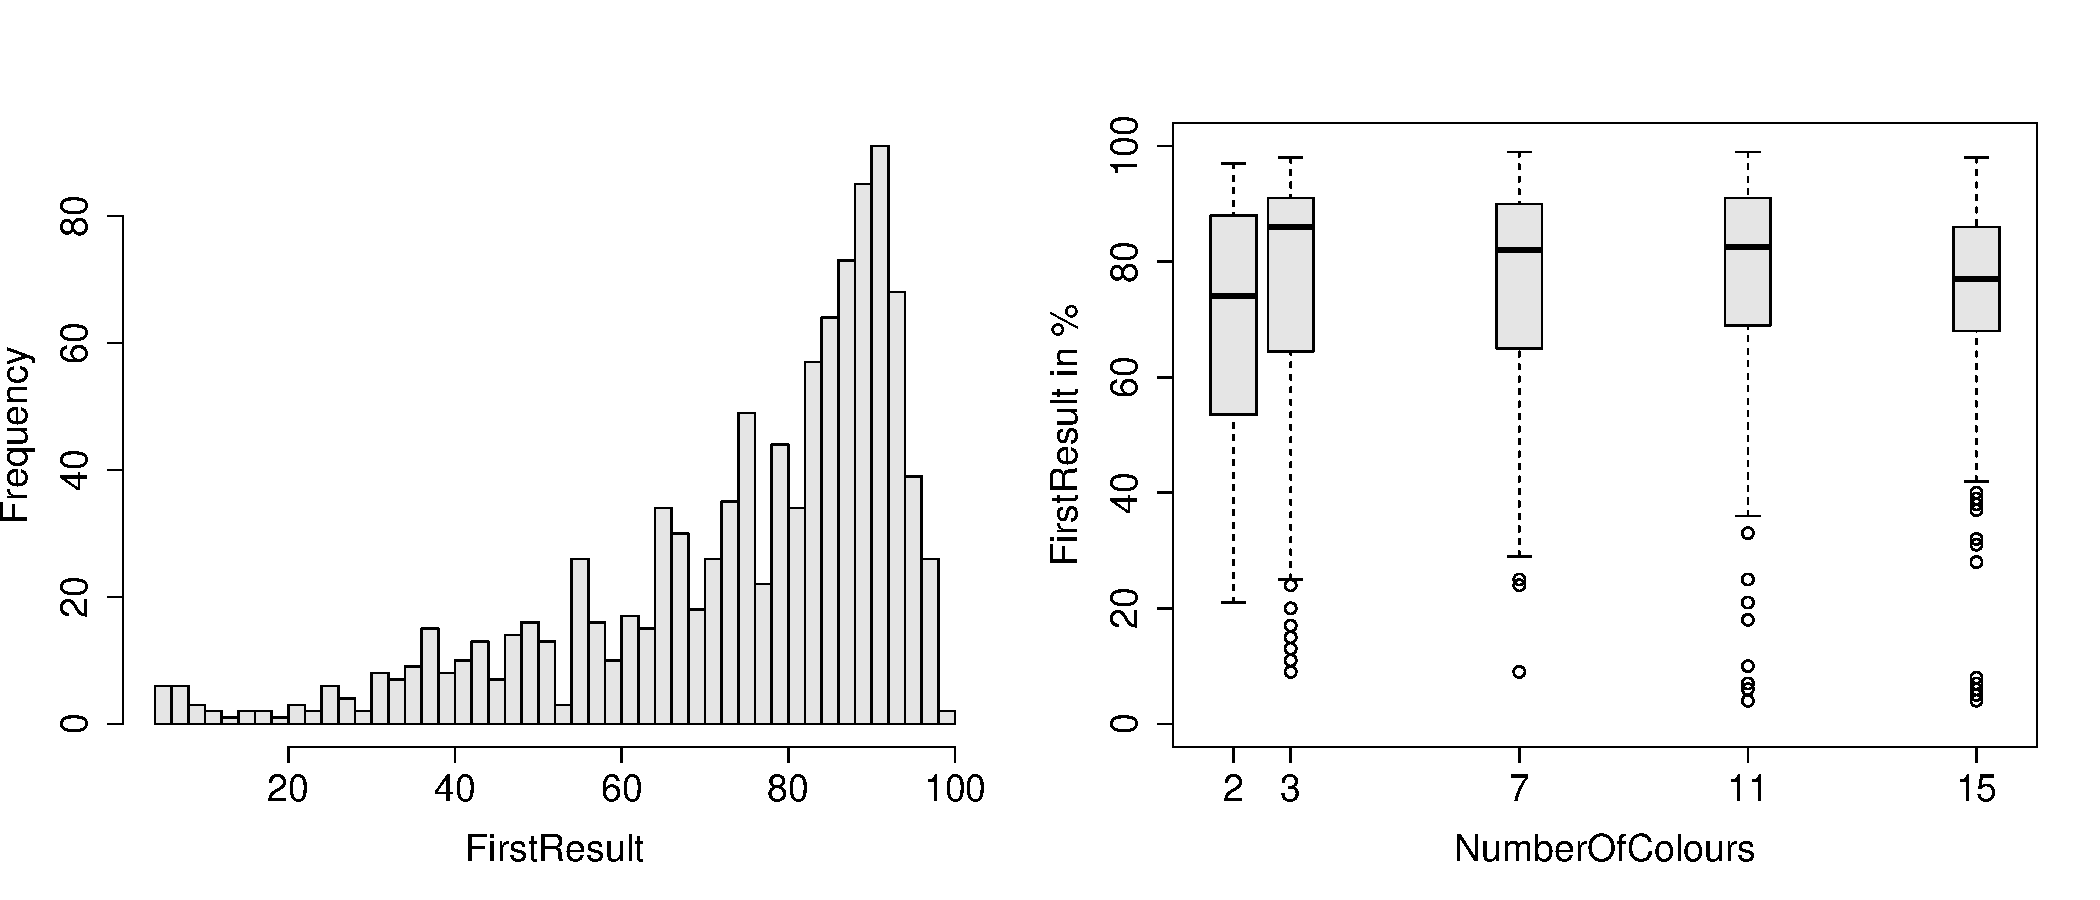
\includegraphics[height = 0.38\textwidth]{DescriptivesFirstResult.pdf}
  \caption{FirstResult - Histogram and Box plot}
    \label{DistributionFirstResult} 
\end{center}
\end{figure}

\begin{figure}[htbp] % DistributionBestResult
\begin{center} 
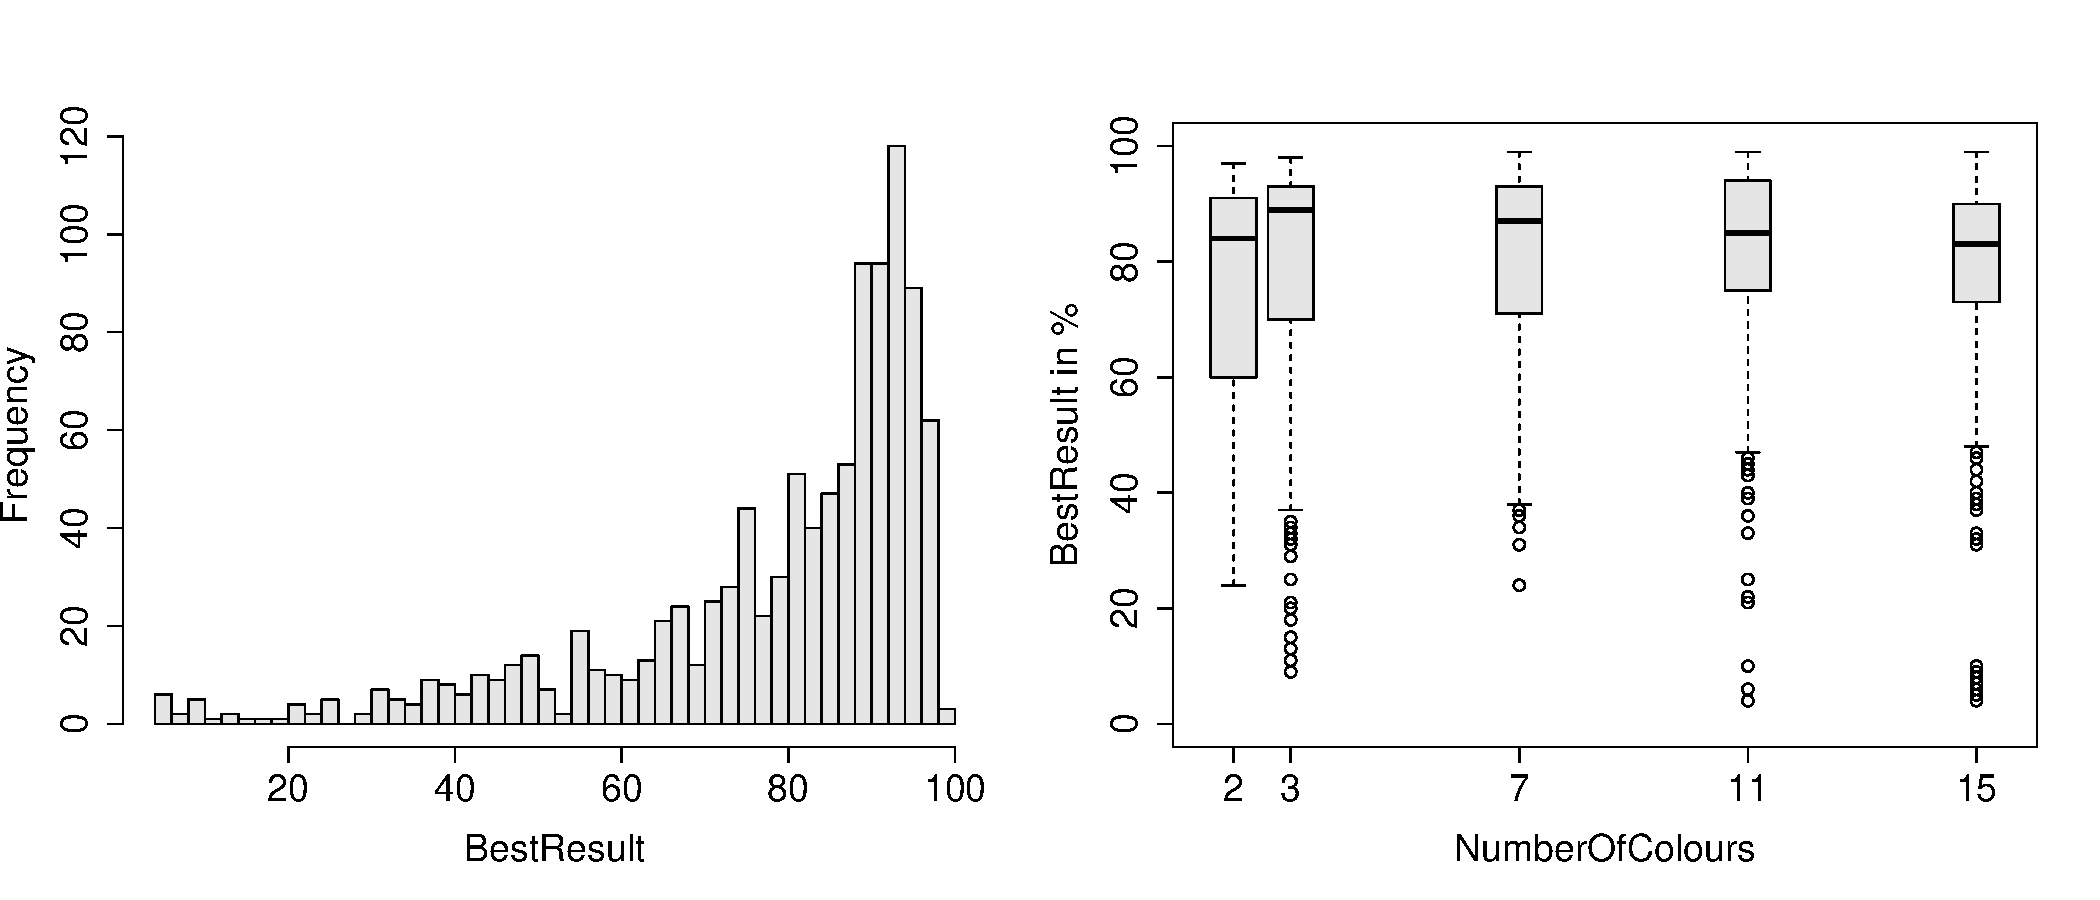
\includegraphics[height = 0.38\textwidth]{DescriptivesBestResult.pdf}
  \caption{BestResult - Histogram and Box plot}
    \label{DistributionBestResult} 
\end{center}
\end{figure}

\begin{figure}[htbp] % DistributionFirstTime
\begin{center} 
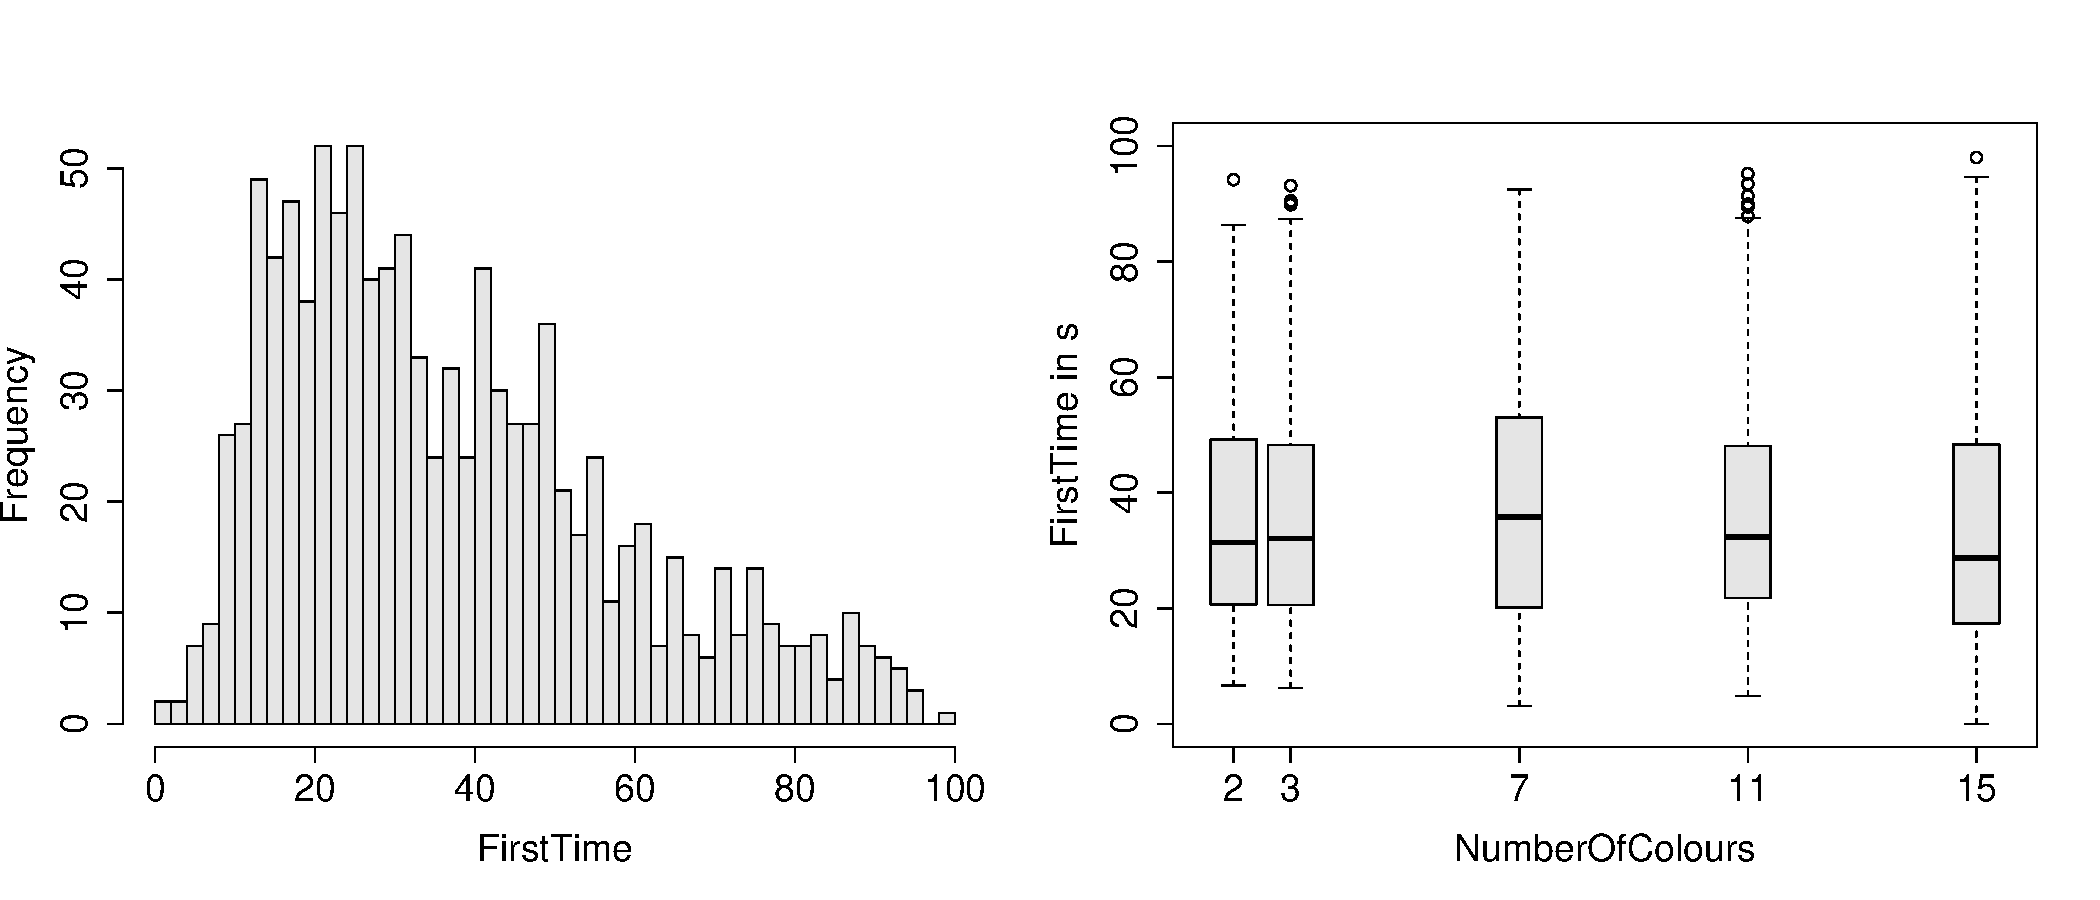
\includegraphics[height = 0.38\textwidth]{DescriptivesFirstTime.pdf}
  \caption{FirstTime - Histogram and Box plot}
    \label{DistributionFirstTime} 
\end{center}
\end{figure}
\begin{figure}[htbp] % DistributionBestTime
\begin{center} 
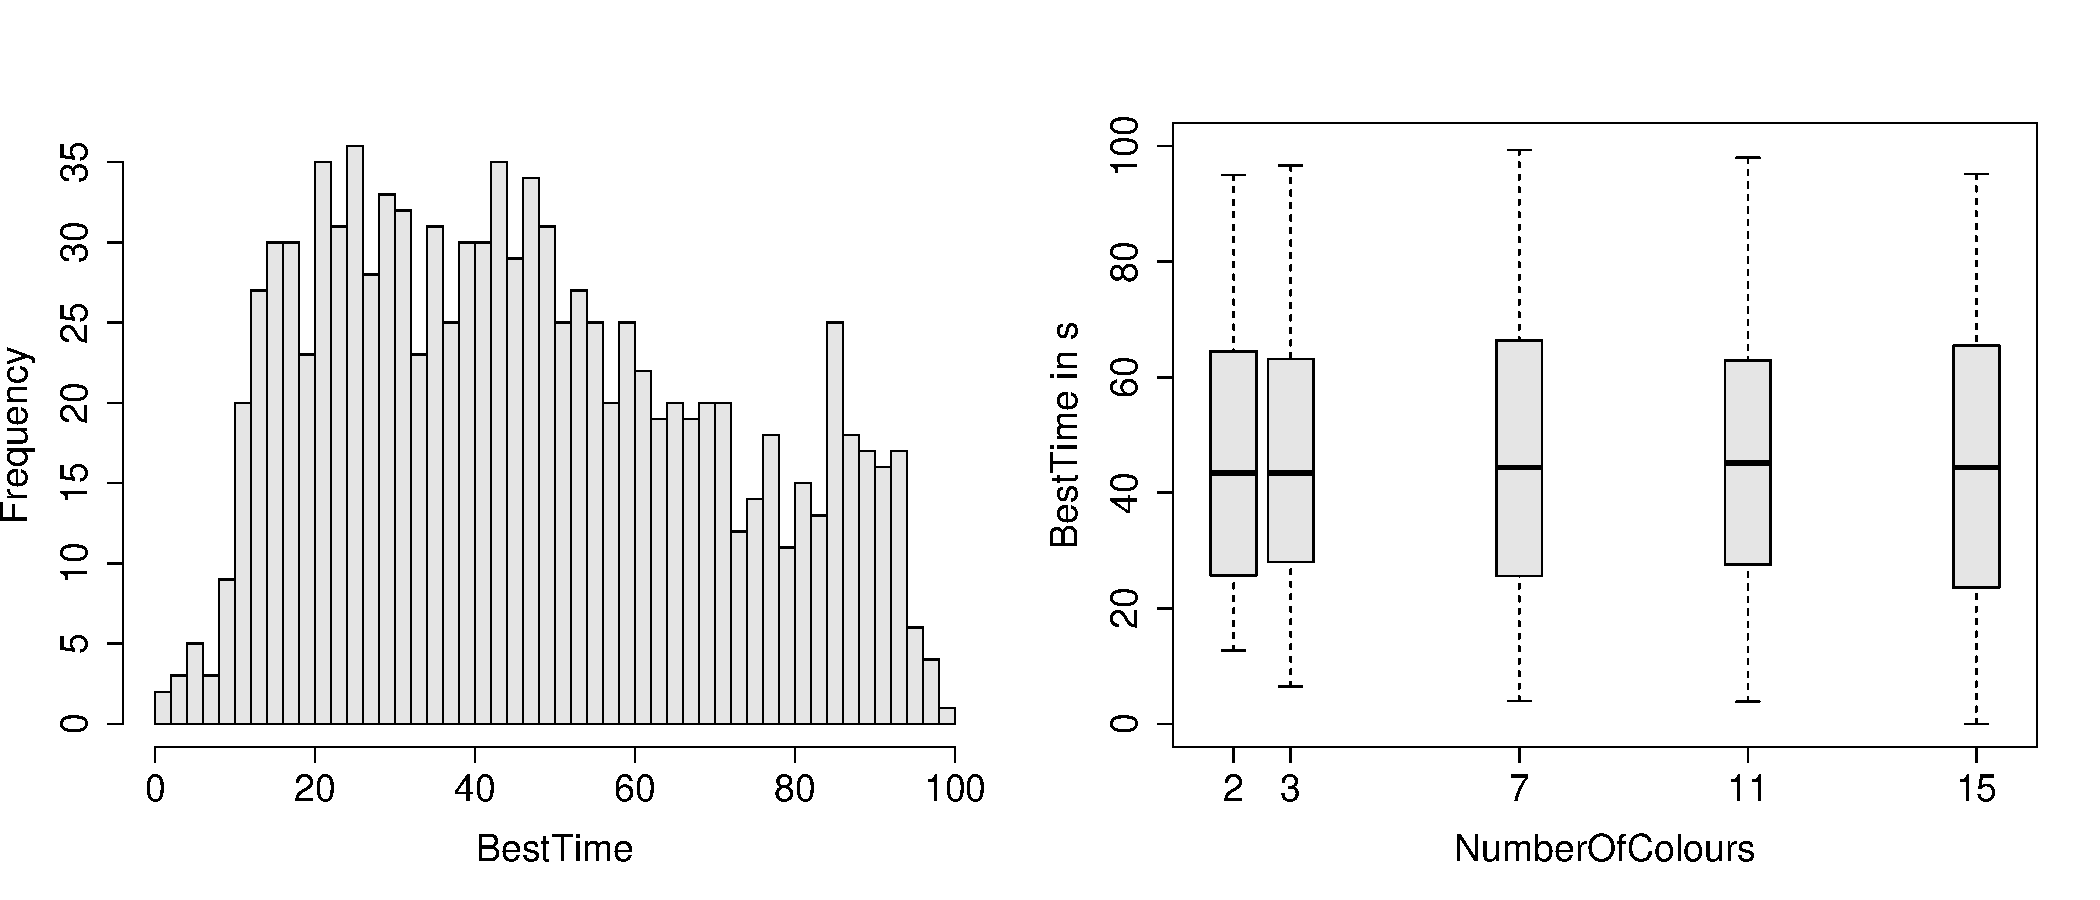
\includegraphics[height = 0.38\textwidth]{DescriptivesBestTime.pdf}
  \caption{BestTime - Histogram and Box plot}
    \label{DistributionBestTime} 
\end{center}
\end{figure}

\begin{figure}[htbp] % DistributionDecisionTime
\begin{center} 
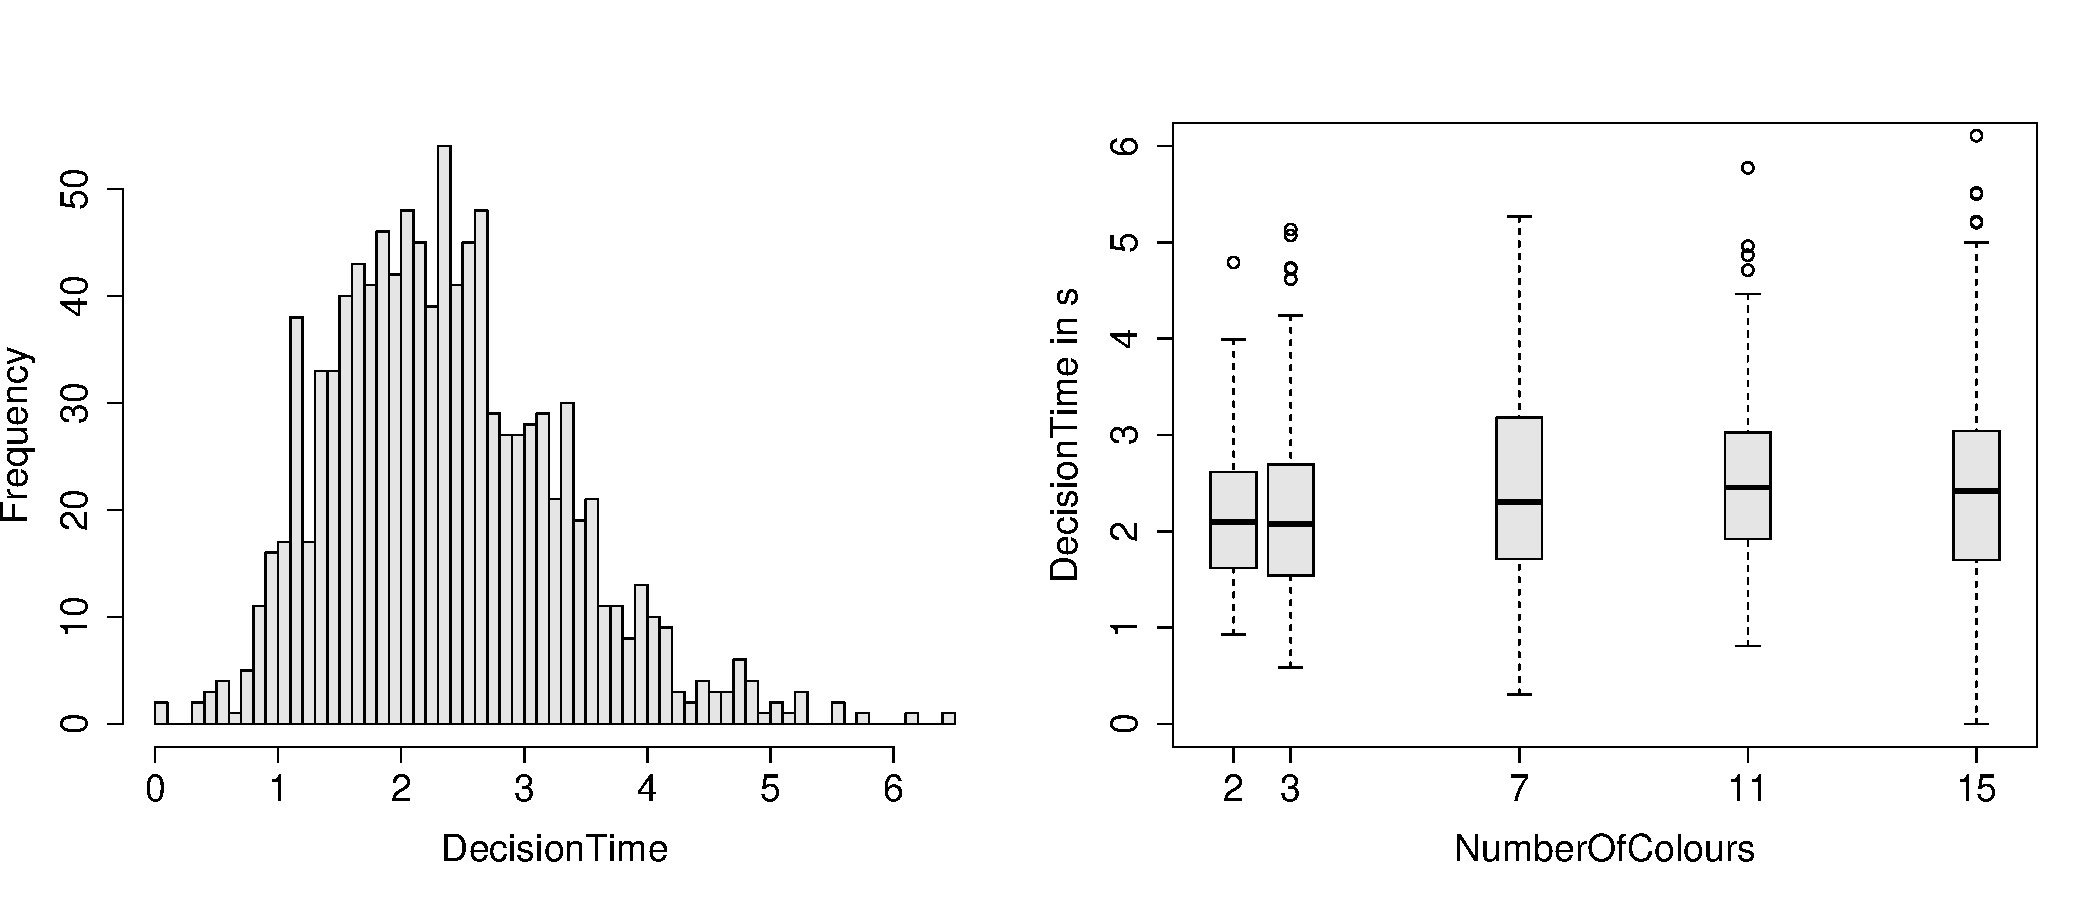
\includegraphics[height = 0.38\textwidth]{DescriptivesDecisionTime.pdf}
  \caption{DecisionTime - Histogram and Box plot}
    \label{DistributionDecisionTime} 
\end{center}
\end{figure}

\begin{figure}[htbp] % DistributionDecisionTime
\begin{center} 
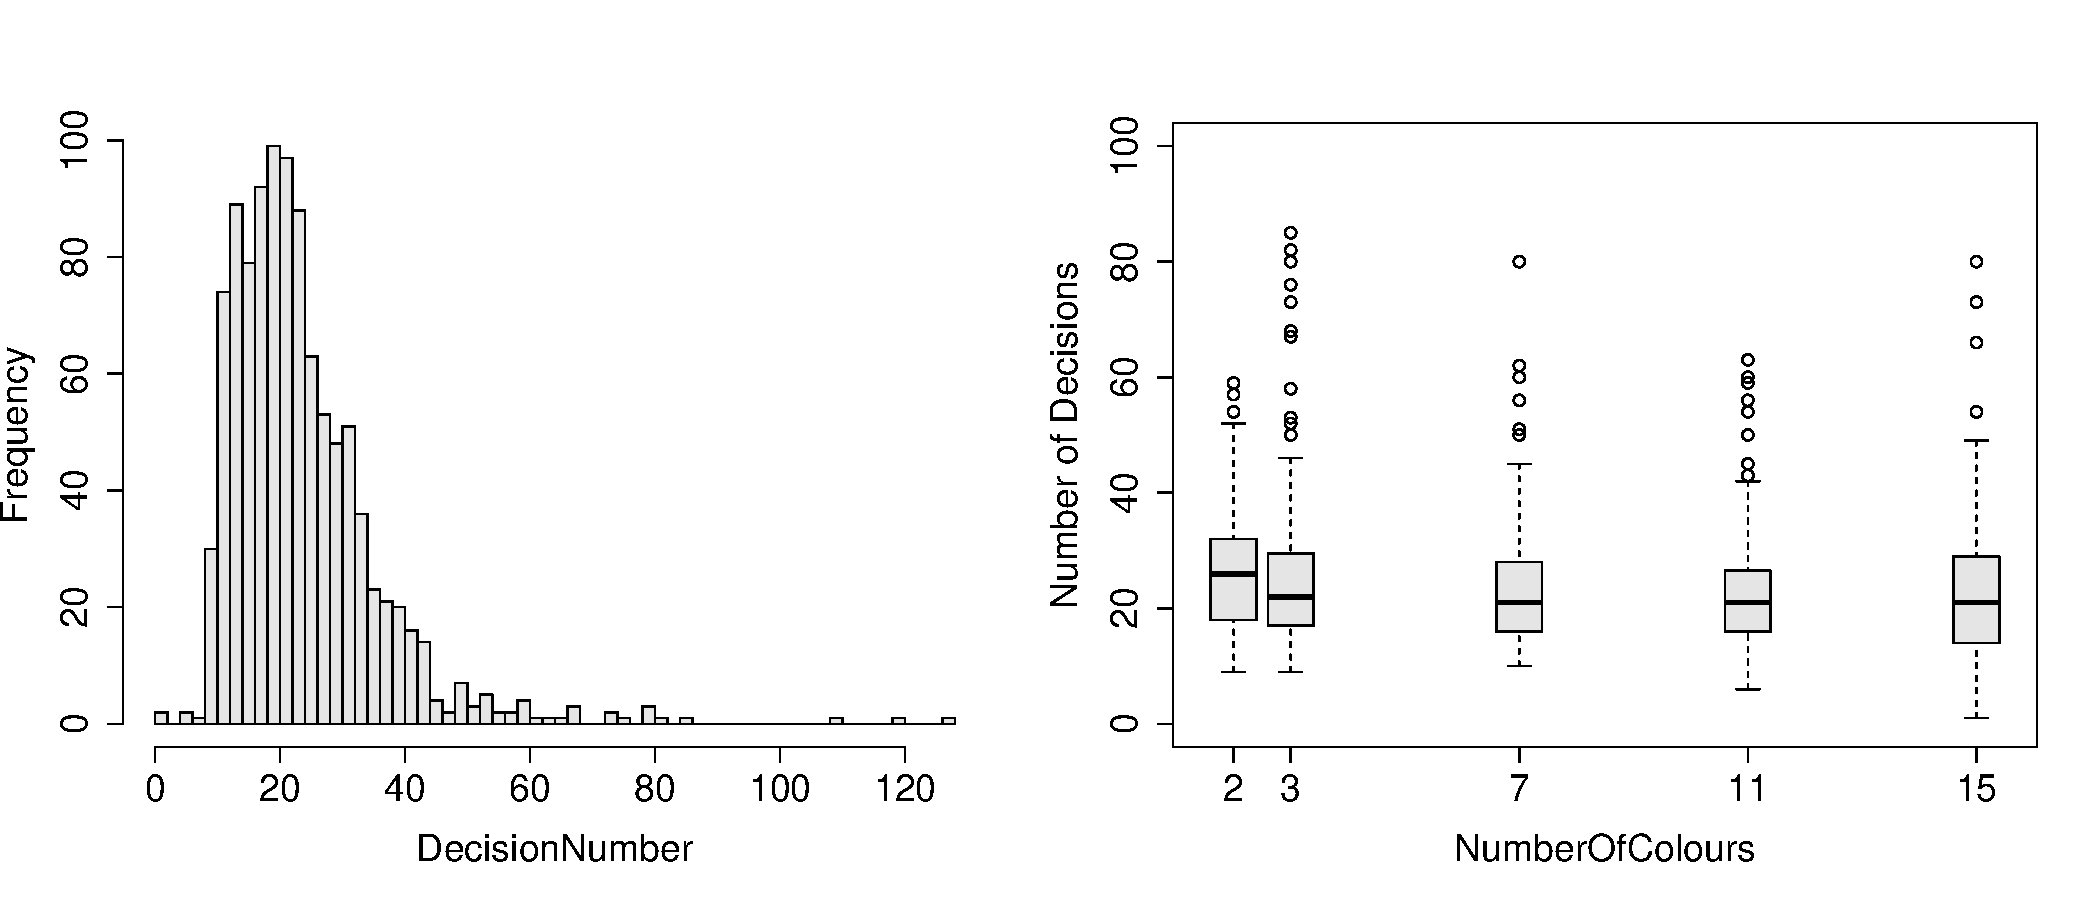
\includegraphics[height = 0.38\textwidth]{DescriptivesDecisionNumber.pdf}
  \caption{DecisionNumber - Histogram and Box plot}
    \label{DistributionDecisionNumber} 
\end{center}
\end{figure}

\begin{figure}[!ht] % Question1
\centering
  \caption[Question 1 - Histogram and Box plot]{Question 1 - very low (1) to very high (7)}
    \label{Question1}  
\begin{subfigure} 
\centering
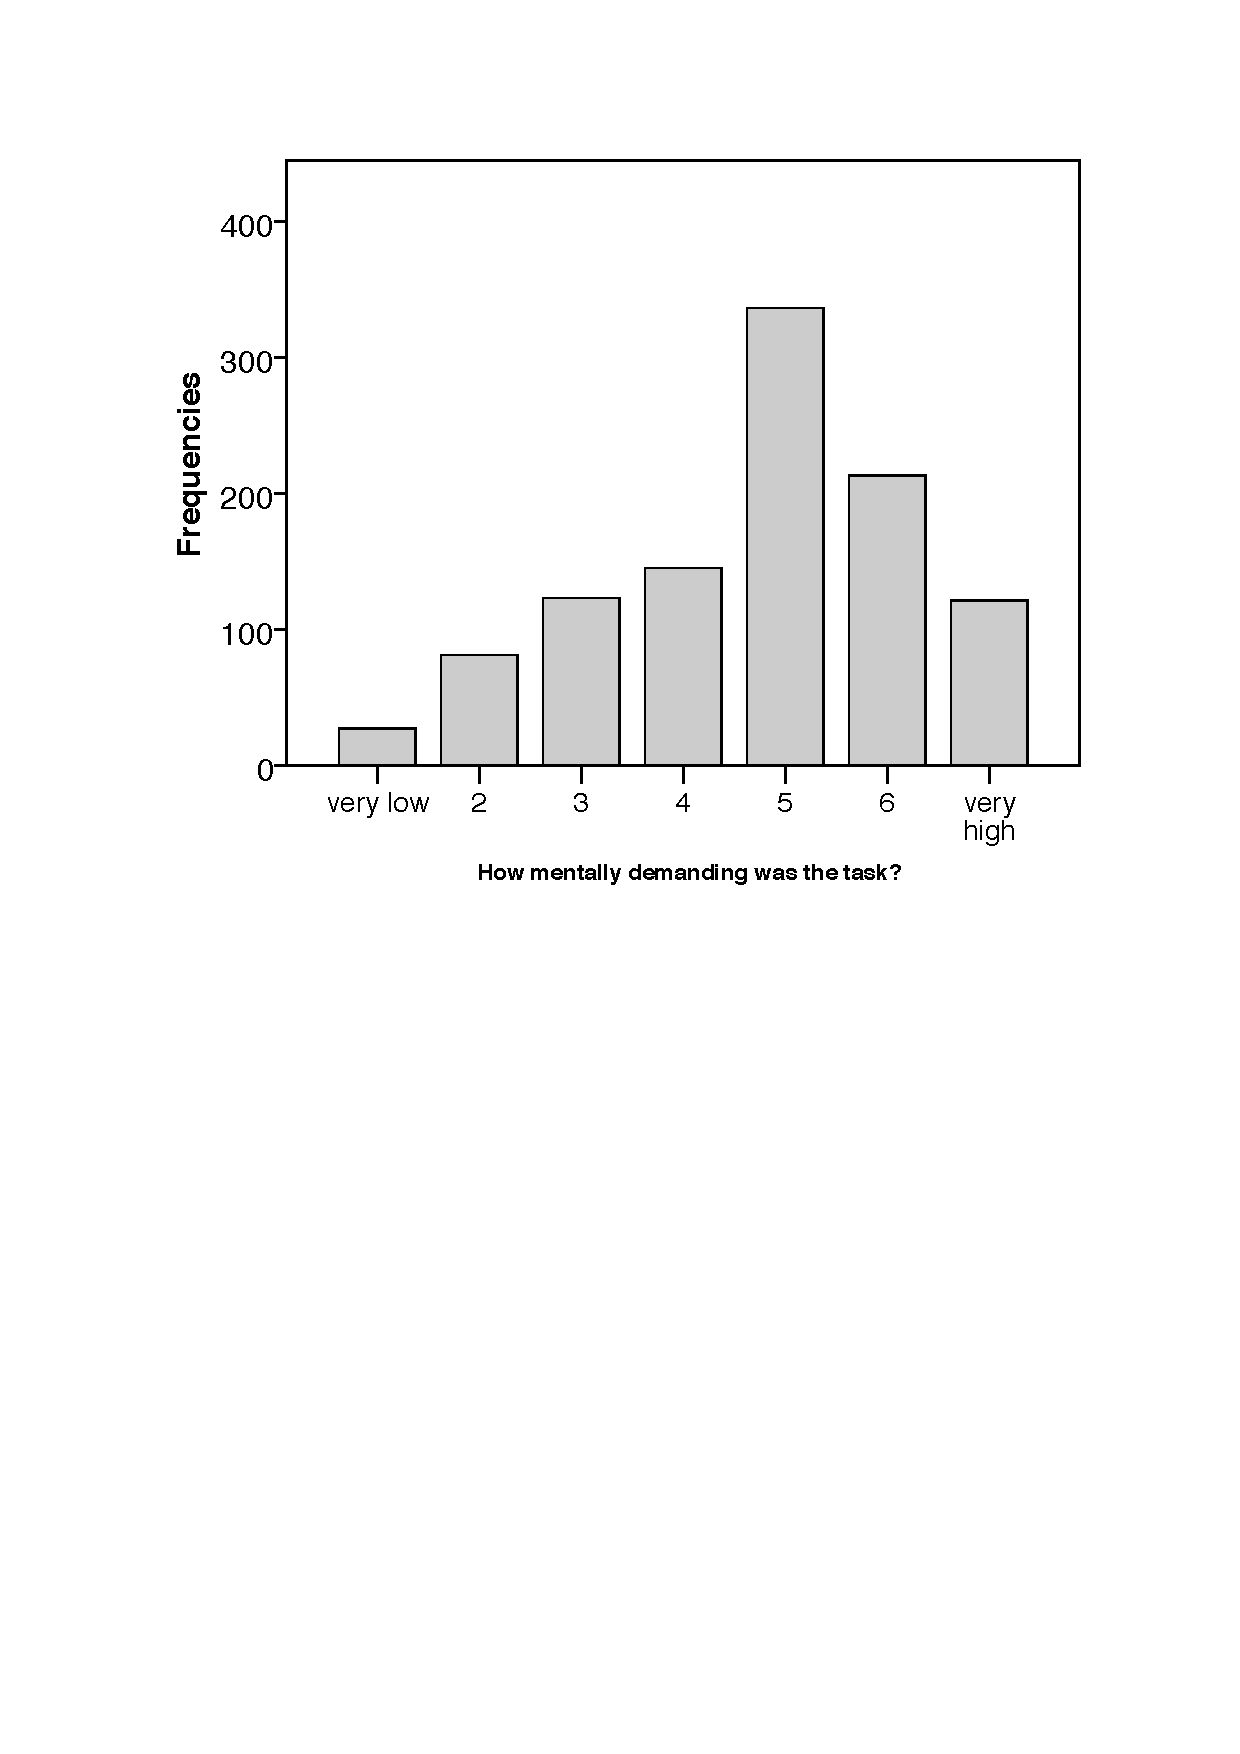
\includegraphics[height = 0.38\textwidth]{HistogramQuestion1.pdf}
\end{subfigure} 
\begin{subfigure} 
\centering
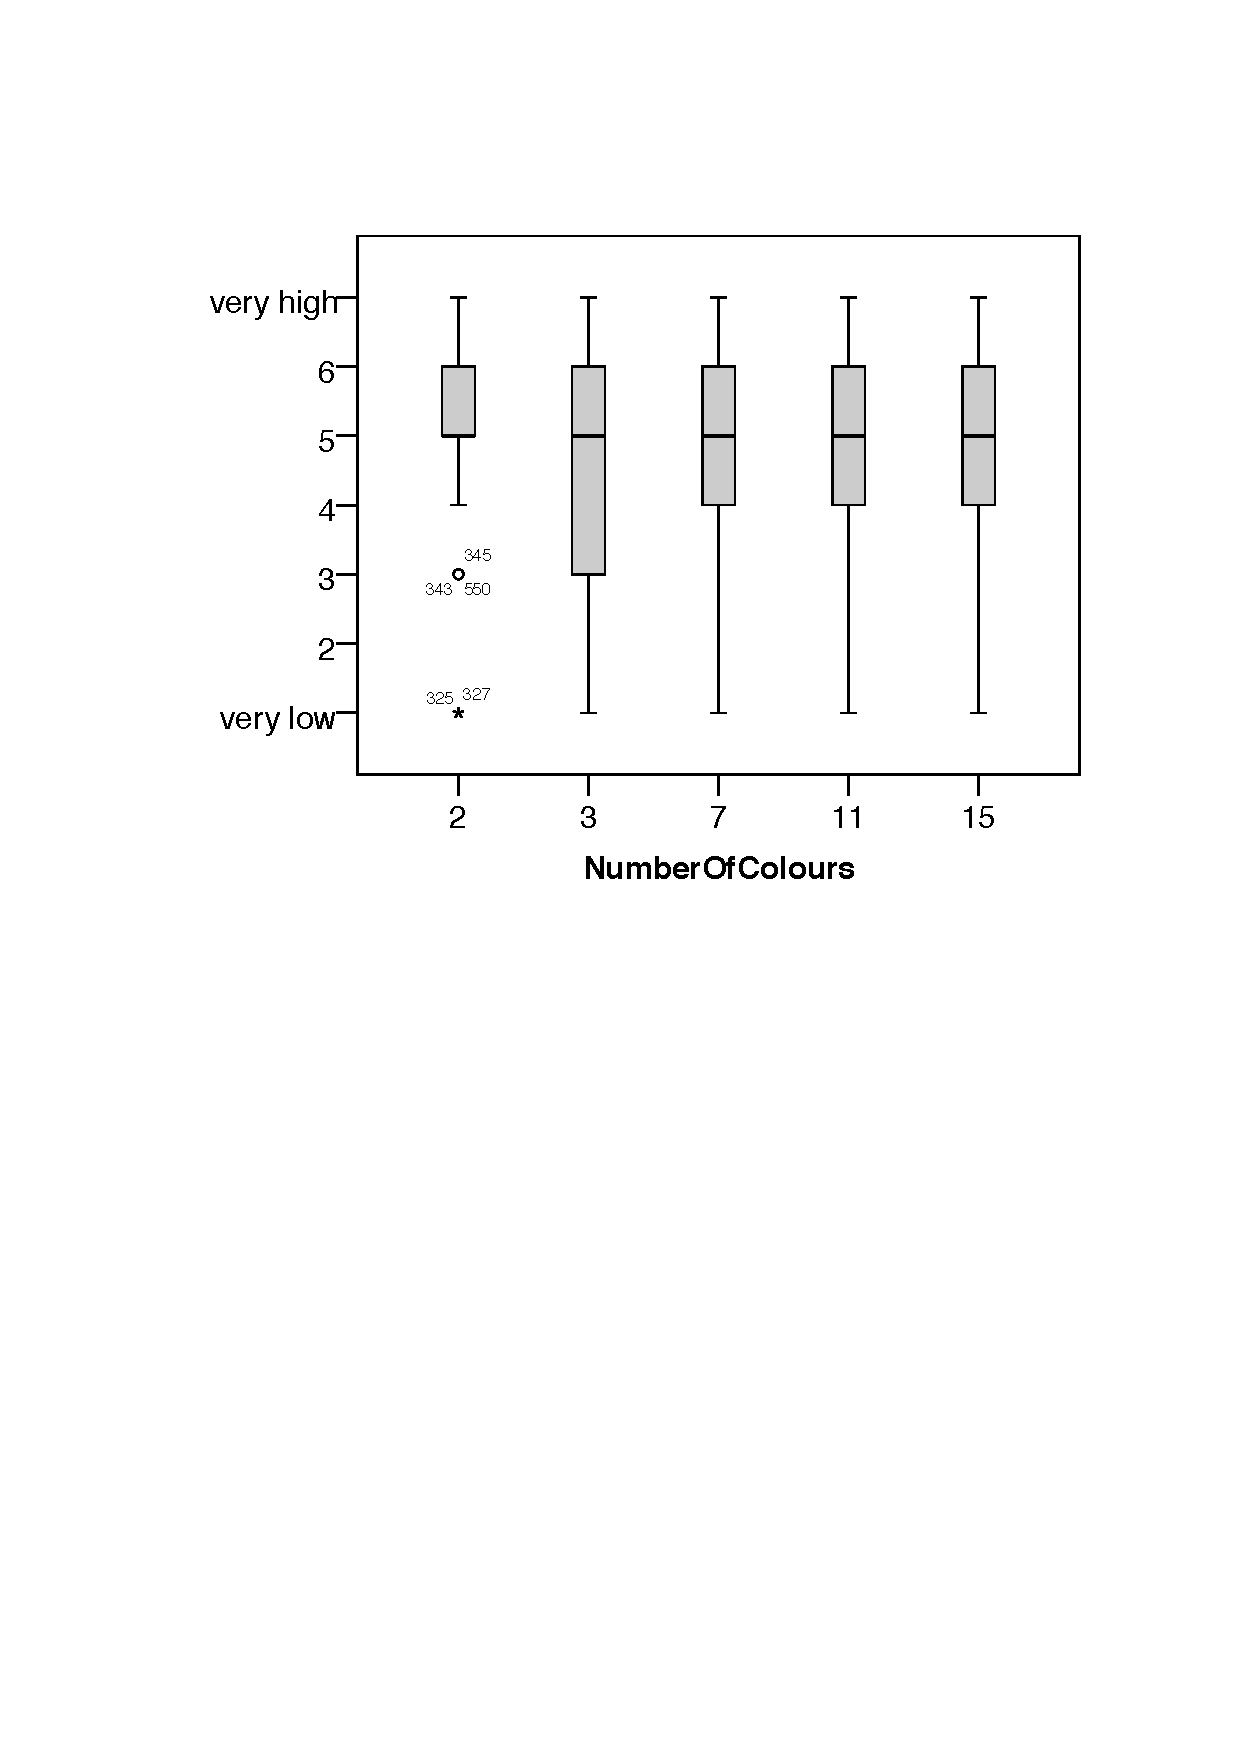
\includegraphics[height = 0.38\textwidth]{BoxplotQuestion1.pdf}
\end{subfigure}
\end{figure}
\begin{figure}[H] % Question2	
\begin{center} 
\begin{subfigure} 
\centering
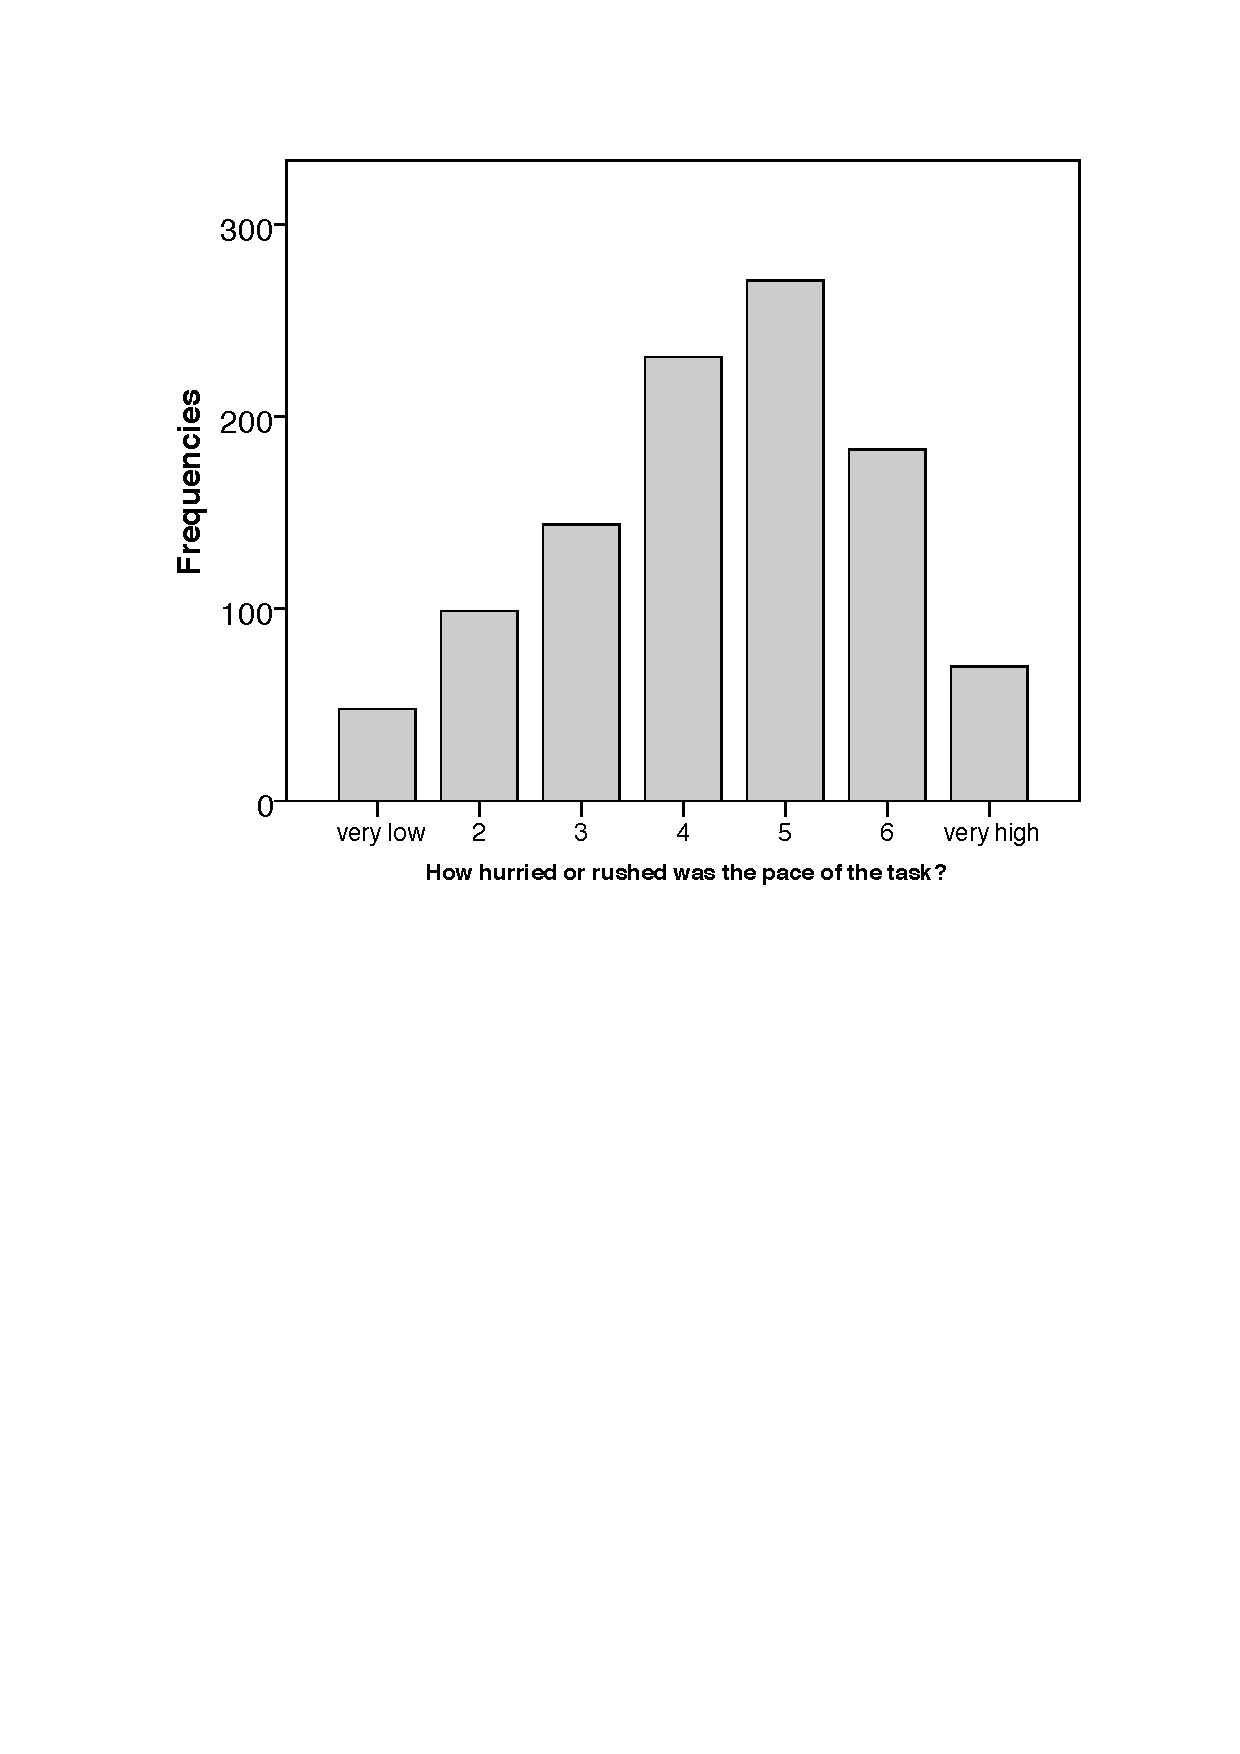
\includegraphics[height = 0.38\textwidth]{HistogramQuestion2.pdf}
\end{subfigure} 
\begin{subfigure} 
\centering
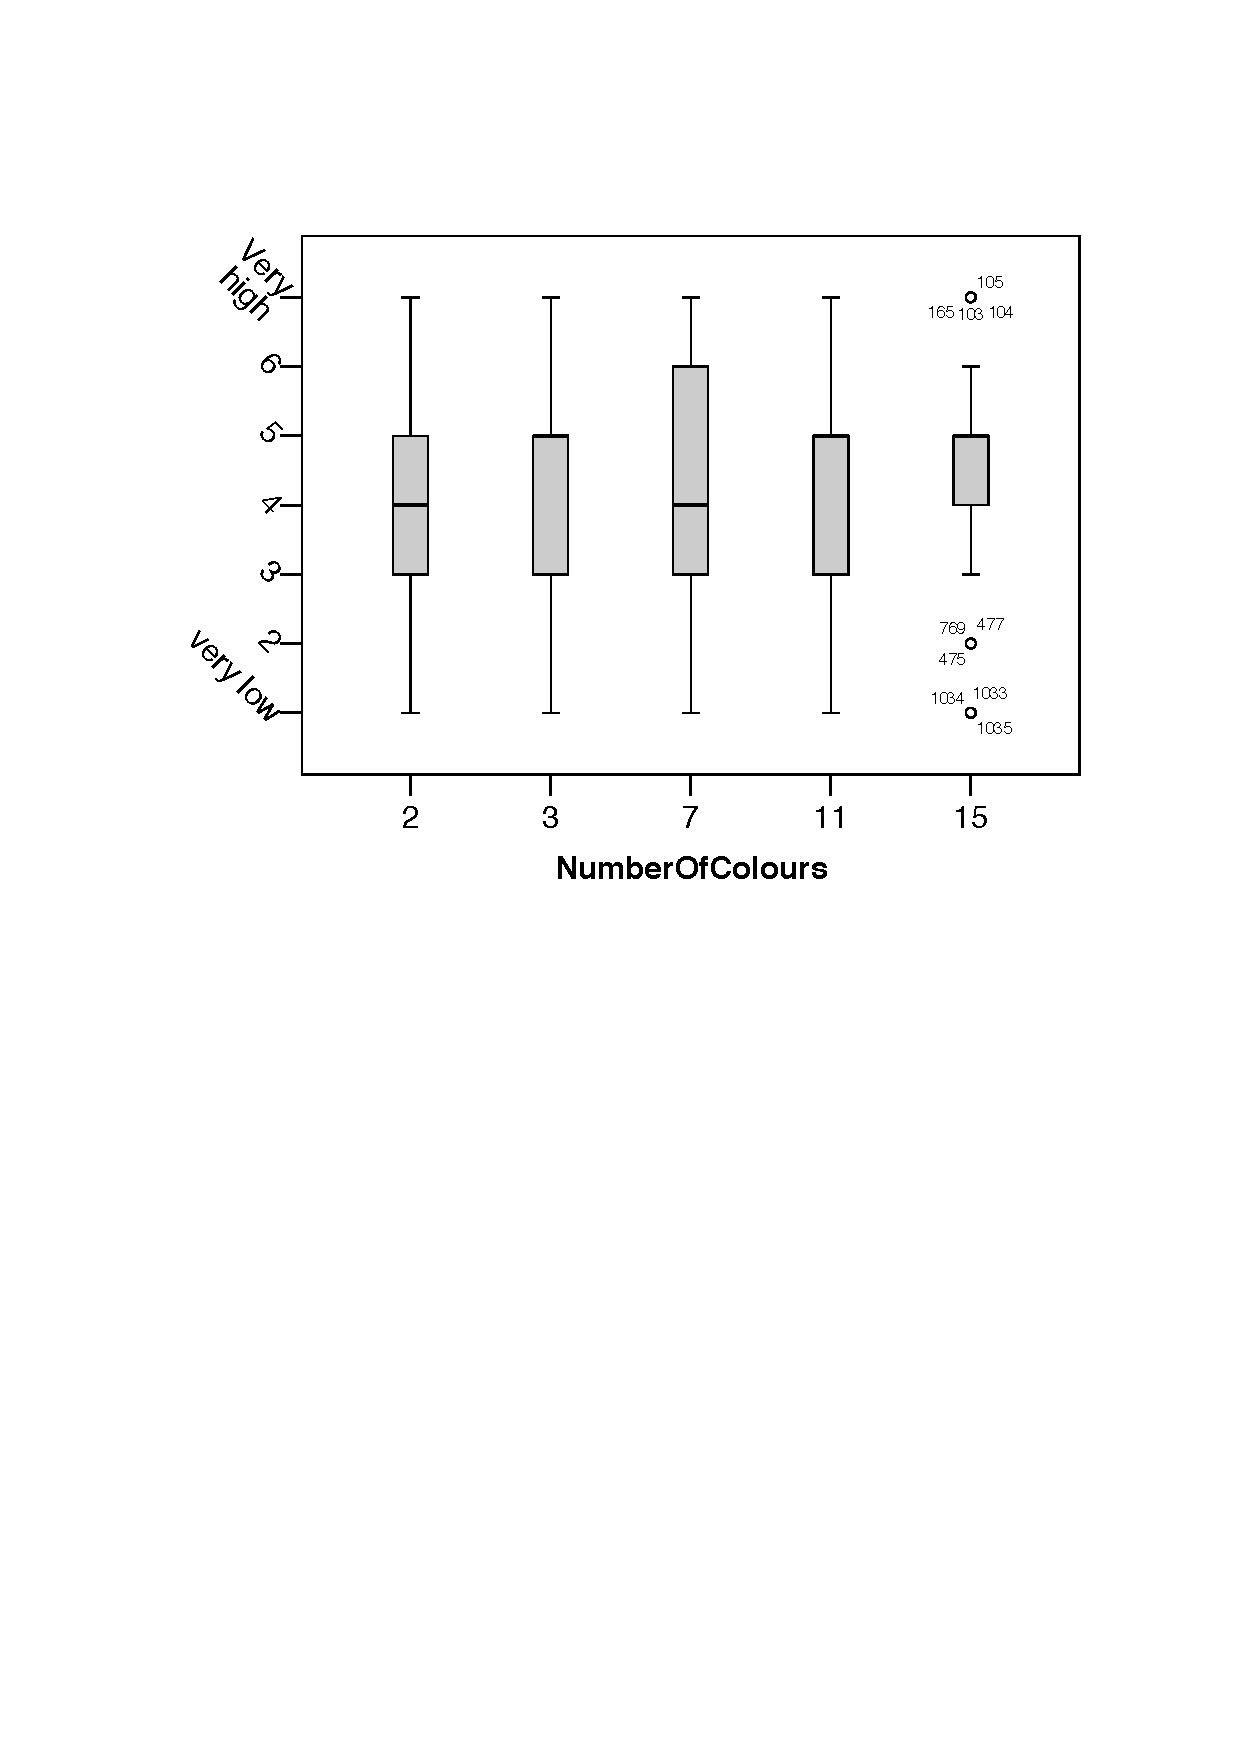
\includegraphics[height = 0.38\textwidth]{BoxplotQuestion2.pdf}
\end{subfigure}
  \caption[Question 2 - Histogram and Box plot]{Question 2 - very low (1) to very high (7)}
    \label{Question2} 
\end{center}
\end{figure}
\begin{figure}[htbp] % Question3	
\begin{center} 
\begin{subfigure} 
\centering
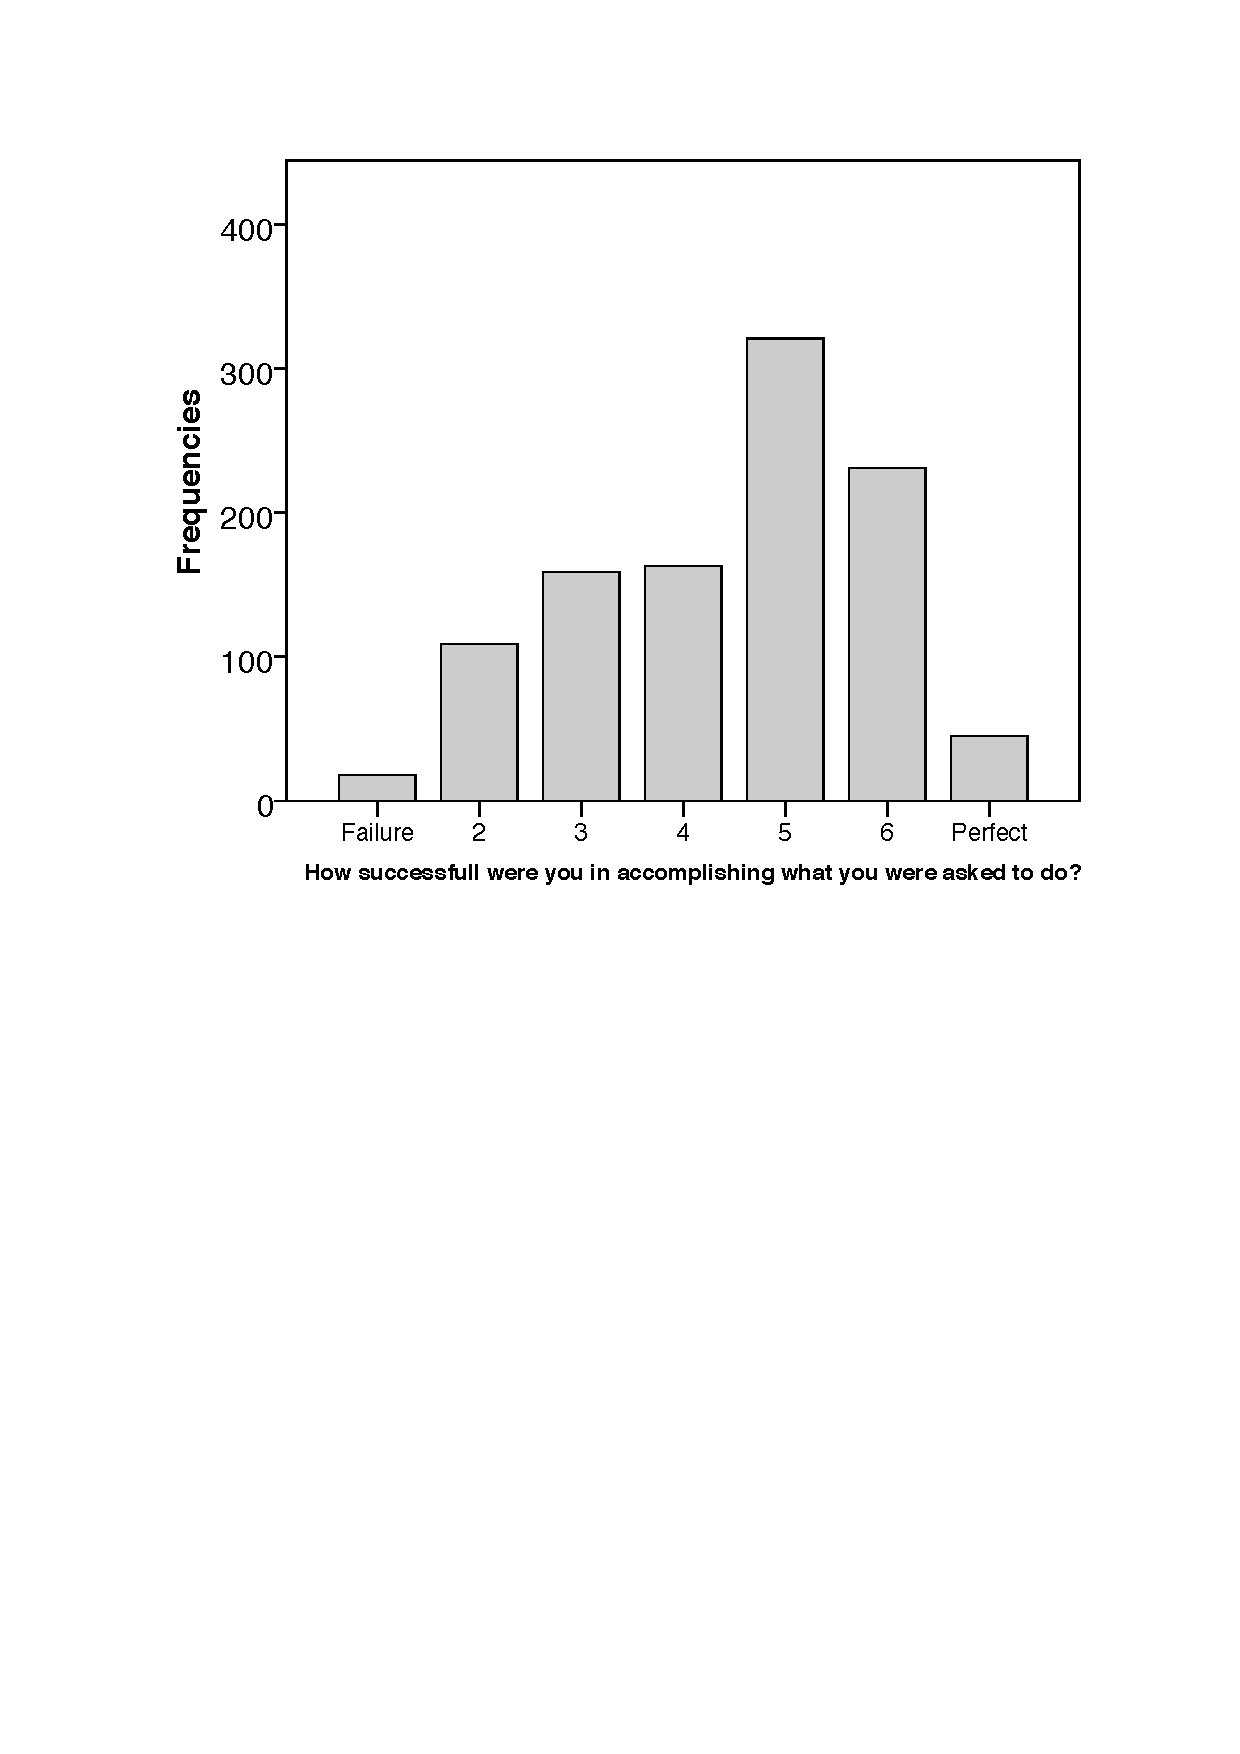
\includegraphics[height = 0.35\textwidth]{HistogramQuestion3.pdf}
\end{subfigure} 
\begin{subfigure} 
\centering
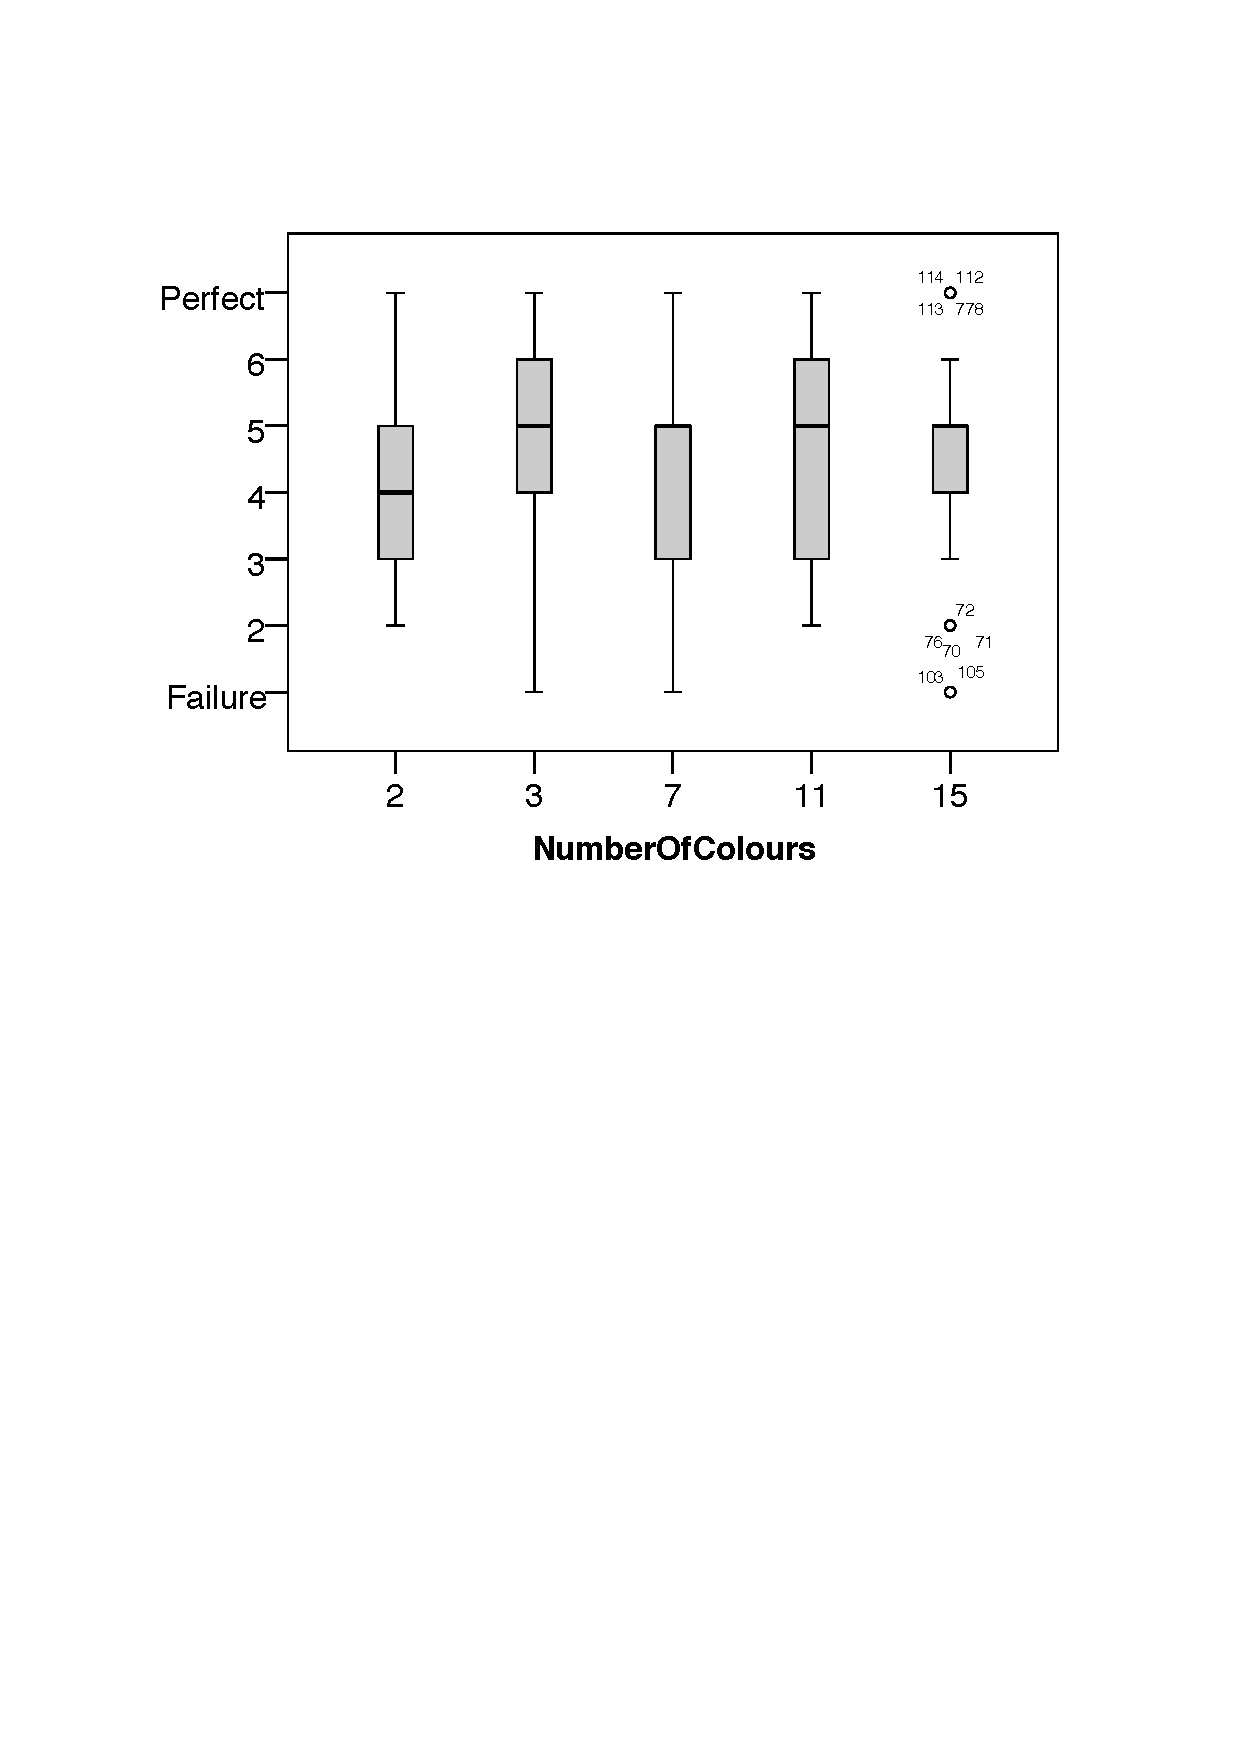
\includegraphics[height = 0.35\textwidth]{BoxplotQuestion3.pdf}
\end{subfigure}
  \caption[Question 3 - Histogram and Box plot]{Question 3 - Failure (1) to Perfect (7)}
    \label{Question3} 
\end{center}
\end{figure}
\begin{figure}[htbp] % Question4	
\begin{center} 
\begin{subfigure} 
\centering
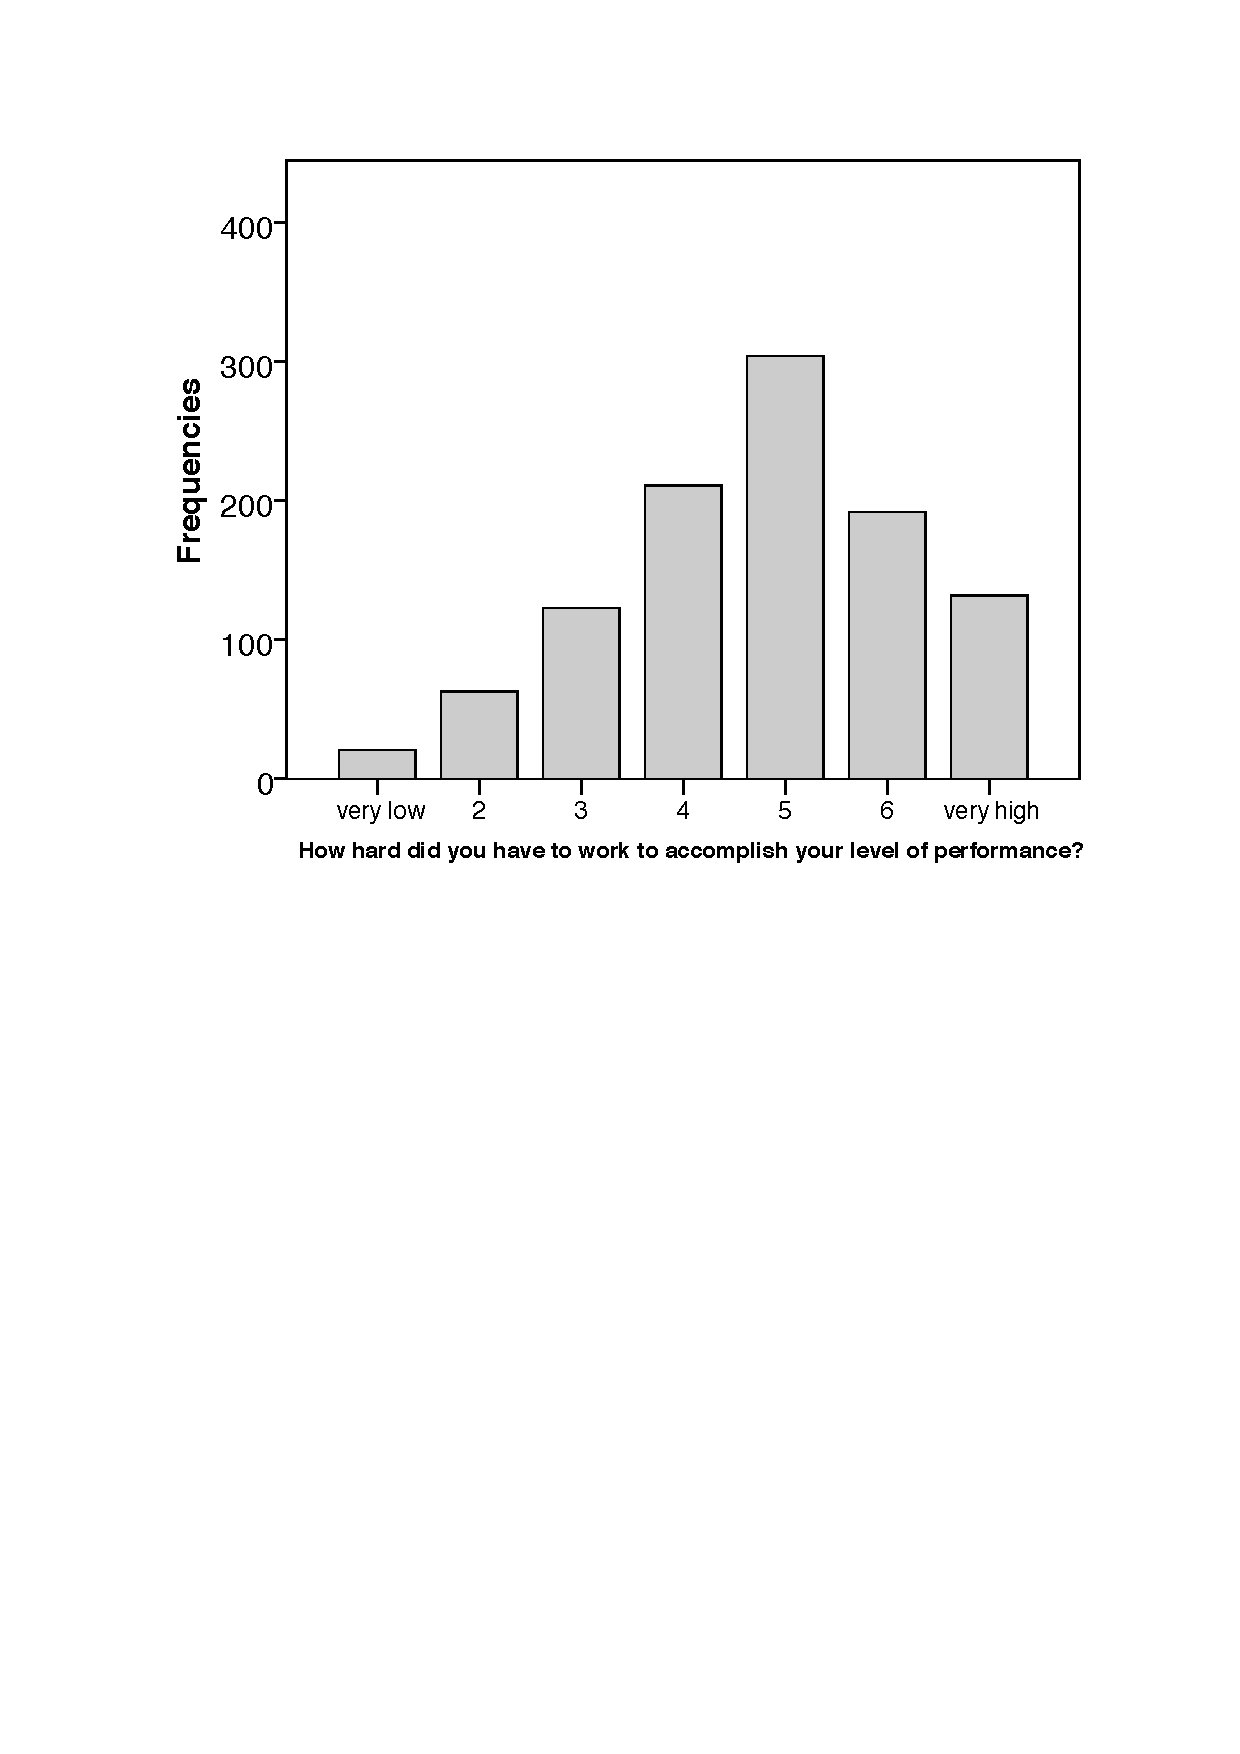
\includegraphics[height = 0.35\textwidth]{HistogramQuestion4.pdf}
\end{subfigure} 
\begin{subfigure} 
\centering
\includegraphics[height = 0.35\textwidth]{BoxplotQuestion4.pdf}
\end{subfigure}
  \caption[Question 4 - Histogram and Box plot]{Question 4 - very low (1) to very high (7}
    \label{Question4} 
\end{center}
\end{figure}
\begin{figure}[htbp] % Question5	
\begin{center} 
\begin{subfigure} 
\centering
\includegraphics[height = 0.35\textwidth]{HistogramQuestion5.pdf}
\end{subfigure} 
\begin{subfigure} 
\centering
\includegraphics[height = 0.35\textwidth]{BoxplotQuestion5.pdf}
\end{subfigure}
  \caption[Question 5 - Histogram and Box plot]{Question 5 - very low (1) to very high (7)}
    \label{Question5} 
\end{center}
\end{figure}
\begin{figure}[htbp] % Question6	
\begin{center} 
\begin{subfigure} 
\centering
\includegraphics[height = 0.38\textwidth]{HistogramQuestion6.pdf}
\end{subfigure} 
\begin{subfigure} 
\centering
\includegraphics[height = 0.38\textwidth]{BoxplotQuestion6.pdf}
\end{subfigure}
  \caption[Question 6 - Histogram and Box plot]{Question 6 - Size (1), Colour (2), Combination (3), Other (4), None (5)}
    \label{Question6} 
\end{center}
\end{figure}
		
% Table generated by Excel2LaTeX from sheet 'Sheet1'
\begin{landscape}
\begin{table}[htbp]
  \centering
  \caption{Descriptive Statistics}
  \label{tab:DescriptiveStatistics}%
    \begin{tabular}{c|c|c|c|c|c|c|c|c|c|c|c}
    \multirow{2}[3]{*}{Variable} & \multirow{2}[3]{*}{Range} & \multirow{2}[3]{*}{Minimum} & \multirow{2}[3]{*}{Maximum} & \multicolumn{2}{c|}{Mean} & \multirow{2}[3]{*}{Std. Deviation} & \multirow{2}[3]{*}{Variance} & \multicolumn{2}{c}{Skewness} & \multicolumn{2}{c}{Kurtosis} \bigstrut[b]\\
          &       &       &       & Statistic & Std. Error &       &       & Statistic & Std. Error & \multicolumn{1}{c|}{Statistic} & \multicolumn{1}{c}{Std. Error} \bigstrut\\
    \hline
    FirstResult & 94    & 4     & 98    & 74.7  & 83\%  & 19.3  & 370.6 & -1.29 & 0.11  & 1.44 & 0.21 \bigstrut\\
    \hline
    BestResult & 94    & 4     & 98    & 79.0  & 80\%  & 18.6  & 344.7 & -1.58 & 0.11  & 2.44 & 0.21 \bigstrut\\
    \hline
    FinalResult & 94    & 4     & 98    & 78.3  & 82\%  & 19.0  & 360.0 & -1.51 & 0.11  & 2.12 & 0.21 \bigstrut\\
    \hline
    \end{tabular}%
  \label{tab:addlabel}%
\end{table}%
%\begin{table}[htbp]
%\\
%
%  \centering
%\setlength\doublerulesep{0pt}
%    \caption{Correlation Result - NumberOfColours - Round - ResultTime}
%      \label{tab:Correlation}%
%
%    \begin{tabular}{c|c|c|c|c|c|c|c|c|c}
%    \multirow{2}[0]{*}{Variable} & \multirow{2}[0]{*}{Correlation} & Number of & \multirow{2}[0]{*}{Round} & \multirow{2}[0]{*}{FirstResult} & \multirow{2}[0]{*}{BestResult} & \multirow{2}[0]{*}{FinalResult} & FirstResult & BestResult & FinalResult \\
%          &       & Colours &       &       &       &       & Time  & Time  & Time \\
%          \hline \hline
%    \multirow{2}[1]{*}{FirstResult} & Spearman's rho & -,137** & .033  & \multirow{2}[1]{*}{} & ,927** & ,924** & ,633** & ,425** & ,287** \\
%          & Pearson Correlation & -,108* & .061  &       & ,942** & ,940** & ,522** & ,399** & ,320** \bigstrut[b]\\
%    \hline
%    \multirow{2}[2]{*}{BestResult} & Spearman's rho & -,131** & .040  & ,927** & \multirow{2}[2]{*}{} & ,993** & ,564** & ,540** & ,402** \bigstrut[t]\\
%          & Pearson Correlation & -,093* & .059  & ,942** &       & ,993** & ,456** & ,509** & ,424** \bigstrut[b]\\
%    \hline
%    \multirow{2}[2]{*}{FinalResult} & Spearman's rho & -,129** & .040  & ,924** & ,993** & \multirow{2}[2]{*}{} & ,556** & ,528** & ,363** \bigstrut[t]\\
%          & Pearson Correlation & -,092* & .056  & ,940** & ,993** &       & ,458** & ,502** & ,383** \bigstrut[b]\\
%    \hline
%    \multirow{2}[2]{*}{FirstResultTime} & Spearman's rho & -.076 & -,109* & ,633** & ,564** & ,556** & \multirow{2}[2]{*}{} & ,667** & ,544** \bigstrut[t]\\
%          & Pearson Correlation & -.061 & -,106* & ,522** & ,456** & ,458** &       & ,653** & ,553** \bigstrut[b]\\
%\hline
%\cline{2-10}    \multirow{2}[2]{*}{BestResultTime} & Spearman's rho & -.021 & -.073 & ,425** & ,540** & ,528** & ,667** & \multirow{2}[2]{*}{} & ,788** \bigstrut[t]\\
%          & Pearson Correlation & -.019 & -.072 & ,399** & ,509** & ,502** & ,653** &       & ,791** \bigstrut[b]\\
%    \hline
%    \multirow{2}[2]{*}{FinalResultTime} & Spearman's rho & -.035 & -.037 & ,287** & ,402** & ,363** & ,544** & ,788** & \multirow{2}[2]{*}{} \bigstrut[t]\\
%          & Pearson Correlation & -.036 & -.038 & ,320** & ,424** & ,383** & ,553** & ,791** &  \bigstrut[b]\\
%    \hline \hline
%    \multicolumn{9}{c}{* p < 0.05, ** p < 0.01 level (2-tailed)} \bigstrut\\
%    \end{tabular}%
%\end{table}%
\end{landscape}

%\begin{landscape}
%% Table generated by Excel2LaTeX from sheet 'Sheet1 (2)'
%\begin{table}[htbp]
%  \centering
%  \caption{Correlation Question - Result - NumberOfColours}
%    \label{tab:CorrelationQuestion}%
%    \begin{tabular}{c|c|c|c|c|c|c|c|c|}
%    \multirow{2}[0]{*}{Variable} & \multirow{2}[0]{*}{Correlation} & Number of & \multirow{2}[0]{*}{FirstResult} & \multirow{2}[0]{*}{BestResult} & \multirow{2}[0]{*}{FinalResult} & FirstResult & BestResult & FinalResult \\
%          &       & Colours &       &       &       & Sqr   & Sqr   & Sqr \\
%          \hline \hline
%    \multirow{2}[1]{*}{Question 1} & Spearman's rho & \multirow{2}[1]{*}{0} & \multirow{2}[1]{*}{-- -- **/**} & \multirow{2}[1]{*}{-- -- **/**} & \multirow{2}[1]{*}{-- -- **/**} & \multirow{2}[1]{*}{-- -- **/**} & \multirow{2}[1]{*}{-- -- **/**} & \multirow{2}[1]{*}{-- -- **/**} \\
%          & Pearson Correlation &       &       &       &       &       &       &  \bigstrut[b]\\
%    \hline
%    \multirow{2}[2]{*}{Question 2} & Spearman's rho & \multirow{2}[2]{*}{0} & \multirow{2}[2]{*}{0} & \multirow{2}[2]{*}{0} & \multirow{2}[2]{*}{0} & \multirow{2}[2]{*}{0} & \multirow{2}[2]{*}{0} & \multirow{2}[2]{*}{0} \bigstrut[t]\\
%          & Pearson Correlation &       &       &       &       &       &       &  \bigstrut[b]\\
%    \hline
%    \multirow{2}[2]{*}{Question 3} & Spearman's rho & \multirow{2}[2]{*}{0} & \multirow{2}[2]{*}{+ */*} & \multirow{2}[2]{*}{+ */*} & \multirow{2}[2]{*}{+ */*} & \multirow{2}[2]{*}{+ */*} & \multirow{2}[2]{*}{+ */*} & \multirow{2}[2]{*}{+ */*} \bigstrut[t]\\
%          & Pearson Correlation &       &       &       &       &       &       &  \bigstrut[b]\\
%    \hline
%    \multirow{2}[2]{*}{Question 4} & Spearman's rho & \multirow{2}[2]{*}{0} & \multirow{2}[2]{*}{-- -- **/**} & \multirow{2}[2]{*}{-- -- **/**} & \multirow{2}[2]{*}{-- -- **/**} & \multirow{2}[2]{*}{-- -- **/**} & \multirow{2}[2]{*}{-- -- **/**} & \multirow{2}[2]{*}{-- -- **/**} \bigstrut[t]\\
%          & Pearson Correlation &       &       &       &       &       &       &  \bigstrut[b]\\
%    \hline
%    \multirow{2}[2]{*}{Question 5} & Spearman's rho & \multirow{2}[2]{*}{+ **/**} & \multirow{2}[2]{*}{-- */*} & \multirow{2}[2]{*}{-- */*} & \multirow{2}[2]{*}{-- */*} & \multirow{2}[2]{*}{-- */*} & \multirow{2}[2]{*}{-- */*} & \multirow{2}[2]{*}{-- */*} \bigstrut[t]\\
%          & Pearson Correlation &       &       &       &       &       &       &  \bigstrut[b]\\
%    \hline
%    \multicolumn{9}{c}{** p<0.01, * p<0.05, ++ <0.3, + <0.2, [0.1,-0.1] 0, -- > --0.2, -- -- > -- 0.3} \bigstrut[t]\\
%    \end{tabular}%
%\end{table}%
%\end{landscape}


%% --------------------
%% |   Bibliography   |
%% --------------------
%\cleardoublepage
\phantomsection
\addcontentsline{toc}{chapter}{\bibname}

% IM Style
\iflanguage{english}
{\bibliographystyle{chicago}}	% english style
{\bibliographystyle{chicagode}}	% german style

% Informatik-Style
%\iflanguage{english}
%{\bibliographystyle{IEEEtranSA}}	% english style
%{\bibliographystyle{babalpha-fl}}	% german style
												  
% Use IEEEtran for numeric references
%\bibliographystyle{IEEEtranSA})

\bibliography{thesis}


\end{document}
